This section is based on the results of Mariame Maiga's internship for her 1st year of Masters at Sorbonne Université, which I co-supervised with Frédérique Cheruy from April to July 2025 \citep{maiga2025}. The impact of climate change was studied during the internship but not the effects of irrigation in the future, which was analysed later. All simulations used in this section were run by Frédérique Cheruy. 
Multiple technical issues were encountered to obtain reliable simulations of future climate with and without irrigation, therefore these results remain preliminary.

\hfill

To simulate future climate conditions, the LAM is used with forcing data from a global ICOLMDZOR simulation, under climate change scenario SSP5-8.5, which presents the strongest increase in global mean temperature. 
%todo: FC Tu peux aller chercher un peu de precision dans le papier de Pedro. On utilise des SST et SIC issues de simulations couplées avec l'ocean pour CMIP6 pour faire des simulations forcées en SST et SIC avec GES correspondant au scenario. Mes simulations ont été faites sans aerosols; c est un peu dommage mais comme genere les forçages globaux est tres lourd et que je m en suis rendu compte un peu tard j ai prefere ne pas recommencer + contrainte de temps de Mariame. On peut aussi dire que l on rencontre des difficultes pour utilser directement les sorties CMIP6 à 6h a cause des resolutions laches des simul. globales qui genere des contrasts trop forts entre le LAM et le forçage. On avait vu un moyen de faire avec yan mais j ai oublié et  c etait trop tard pour le stage

The mid-century period 2050-2062 was studied and compared to the present period (2010-2022). Longer simulations are under analysis to extend the study period to 30 years for both present and future but they were not yet available when writing this manuscript.
The smaller LAM domain ($R_{domain} = 1000$ km, $NBP=40$) was used for computational efficiency, considering the findings of Chapter \ref{chap:forcing} that the inconsistencies in the transition zone are limited when lateral boundary conditions are obtained from ICOLMDZOR.
Simulations without irrigation in the present (\presnoirr) and future climate (\futnoirr) are compared to characterize the impacts of climate change over the Peninsula. Then, \futnoirr is compared to a simulation over the same period, with irrigation (\futirr) to analyse how irrigation interacts with these impacts.


\subsection{Impact of climate change over the Iberian Peninsula}

The annual impact of climate change under the SSP5-8.5 scenario on land-atmosphere coupling variables is presented in Fig. \ref{fig:diffmaps_present_future}, as the difference between the \futnoirr (2050-2062) and \presnoirr (2010-2022) simulations. 
%temperature
A general warming of the air is observed, as expected with a strong climate change scenario, with 2-meter temperature increases of 2°C in most of the domain and up to 3°C in the northern half of the Peninsula (Fig. \ref{fig:diffmaps_present_future}a). The coasts are slightly less affected by warming, whereas the mountain ranges are the most impacted regions.
%precip

Precipitation decreases over most of the Peninsula, especially in the northern coast and the Pyrenees while the only region where it increases is the Southeast (Fig. \ref{fig:diffmaps_present_future}c). This region usually receives little precipitation so, although the absolute values are small, the relative increase is higher than 10\% over a large area and exceeds 25\% in several grid cells (see appendix Fig. \ref{fig:reldiffmaps_present_future}). 
%evap and fluxsens
The changes in precipitation translate into similar changes in ET, of lower magnitude (Fig. \ref{fig:diffmaps_present_future}d). The only exceptions are in  Pyrenees and Cantabrian mountain ranges in the North, which are very humid areas where ET is limited by incoming radiation rather than available soil moisture.
These general decreases in precipitation and ET are consistent with CMIP6 projections for the northern Mediterranean basin under climate change, which are attributed to the combined influence of local responses to atmospheric warming and alterations in large-scale circulation patterns \cite{tuel_understanding_2021, arjdal_future_2023}.

The sensible heat flux is increased over almost all the continental domain  (Fig. \ref{fig:diffmaps_present_future}b). This evolution is not only a consequence of changes in surface energy partitioning since increases are also visible in areas where ET is locally increasing. It is likely dominated by an increase in the incoming energy at the surface, since it closely linked to increases in downwelling shortwave radiation (Fig. \ref{fig:diffmaps_present_future}g).
%q2m and RH2m
Near-surface specific humidity is increased over the whole domain, with the largest increases reaching 1 g \perkg on coastal areas (Fig. \ref{fig:diffmaps_present_future}e), which corresponds to a 10\% increase. Considering the increase in 2-meter air temperature, this can be understood using the Clausius-Clapeyron relation, showing that warmer air can contain more water \citep[in theory up to +7\% for a 1°C increase, Chapter 8 in][]{IPCC_2023}.
However, under climate change, the increase in specific humidity is not as impactful as the increase in temperature since 2-meter relative humidity is lower over all the continental domain (Fig. \ref{fig:diffmaps_present_future}f), especially in the north of the Peninsula. 
%link to rad fluxes and cloud cover
This extends to the rest of the atmospheric column and leads to smaller cloud cover (see appendix Fig. \ref{fig:clouds_present_future}), which is reflected by the increase in the downwelling shortwave radiation flux (Fig. \ref{fig:diffmaps_present_future}g), particularly in the north-west of the Peninsula. 
The general increase in longwave downwelling radiation (Fig. \ref{fig:diffmaps_present_future}h) is an expected consequence of a warmer atmosphere, but this increase is not as large in the north and north-west of the domain, where changes in relative humidity (and cloud cover) are the largest . 

%figure : diff maps (no_irr, present - future)
\begin{figure}[htbp]
    \centering
    \begin{tabular}{cc}
        %t2m
        \begin{subfigure}[b]{0.5\textwidth}
            \caption{2-m temperature difference}
            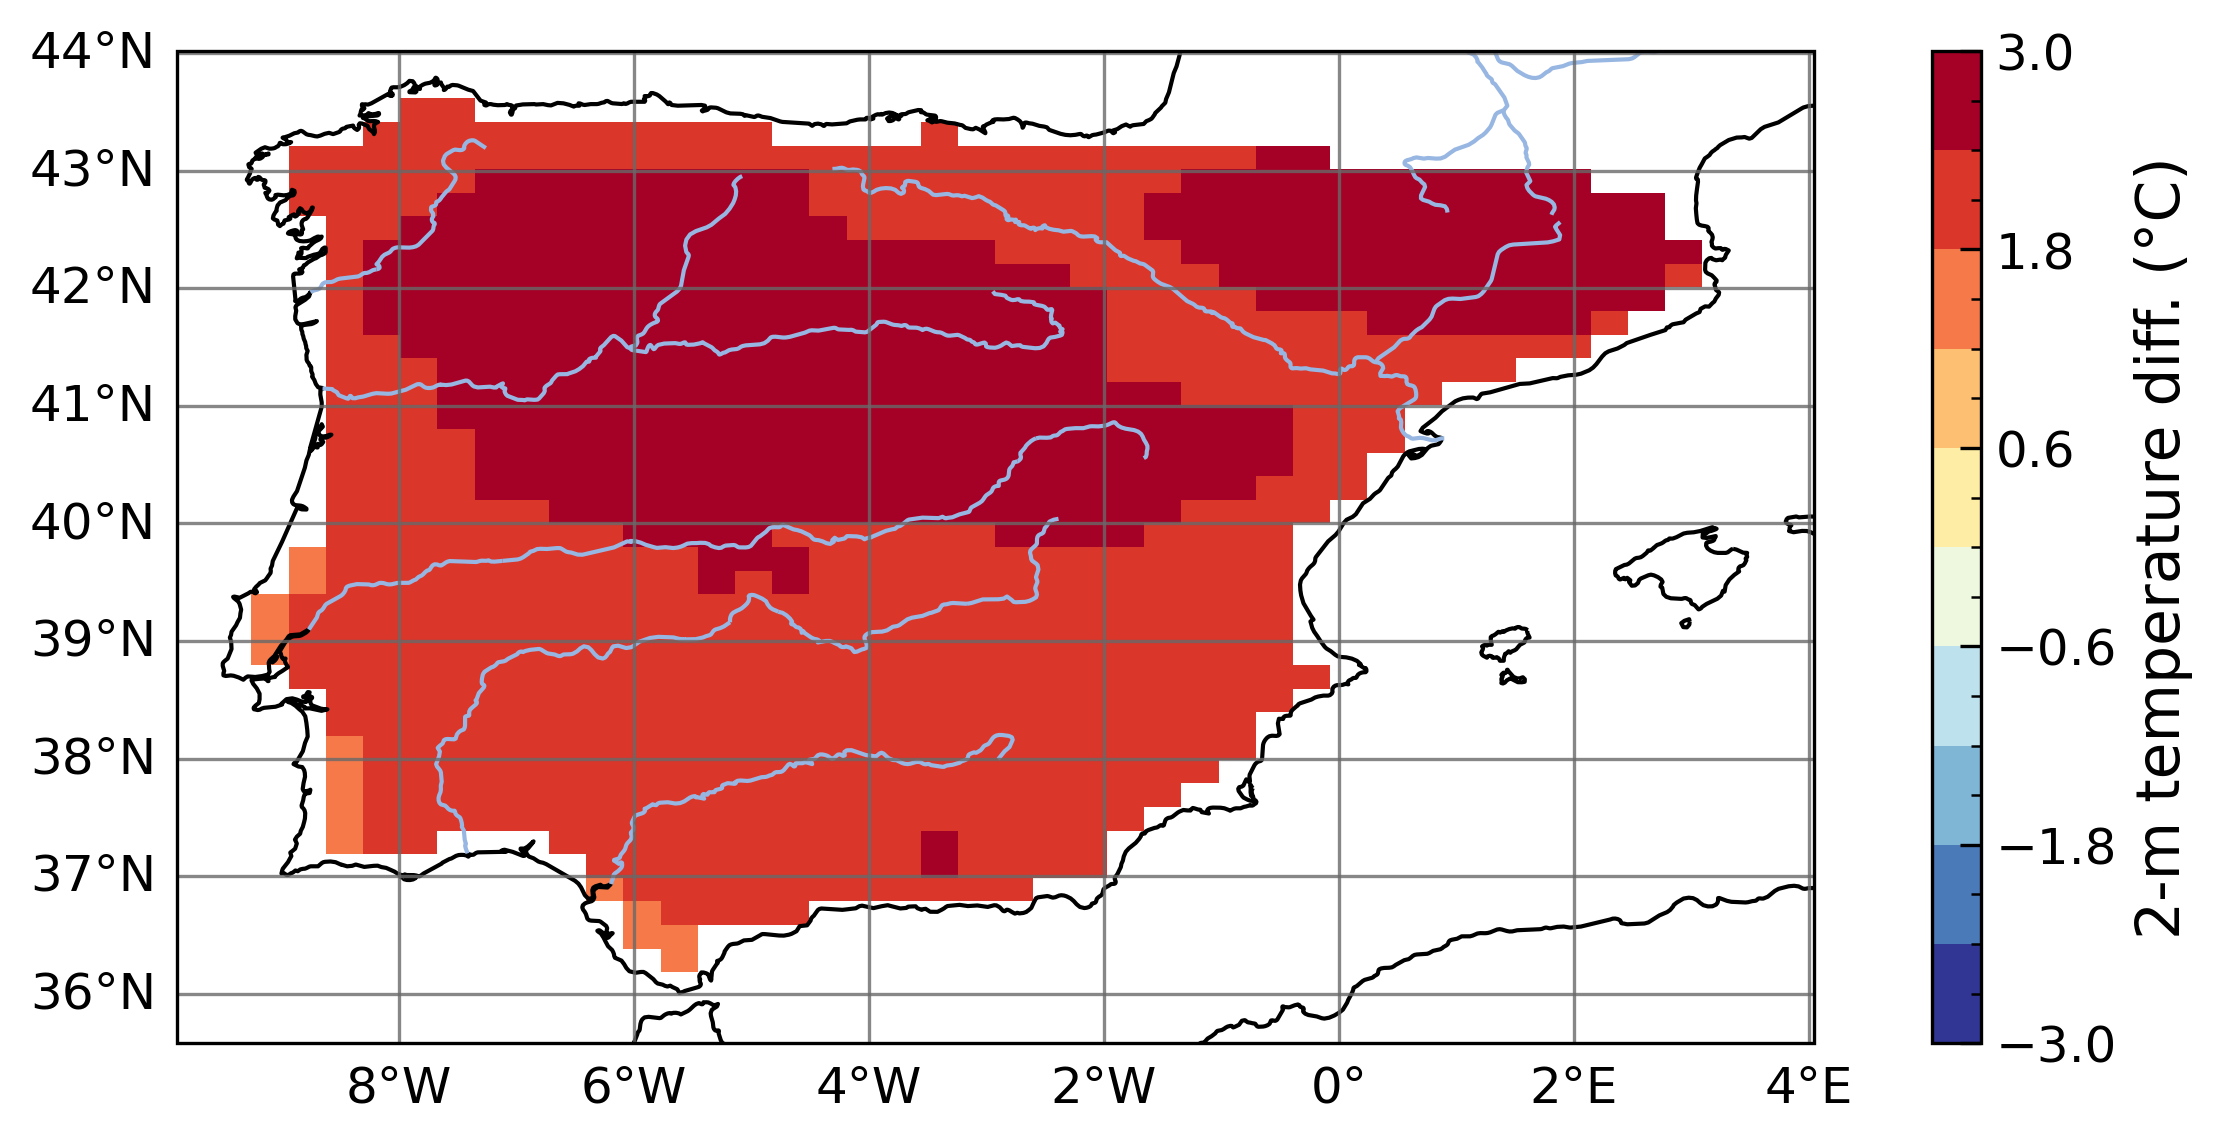
\includegraphics[width=\textwidth]{images/chap4/future/diffmap_t2m_presfut.png}
        \end{subfigure} &
        %fluxsens
        \begin{subfigure}[b]{0.5\textwidth}
            \caption{Sensible heat flux difference}
            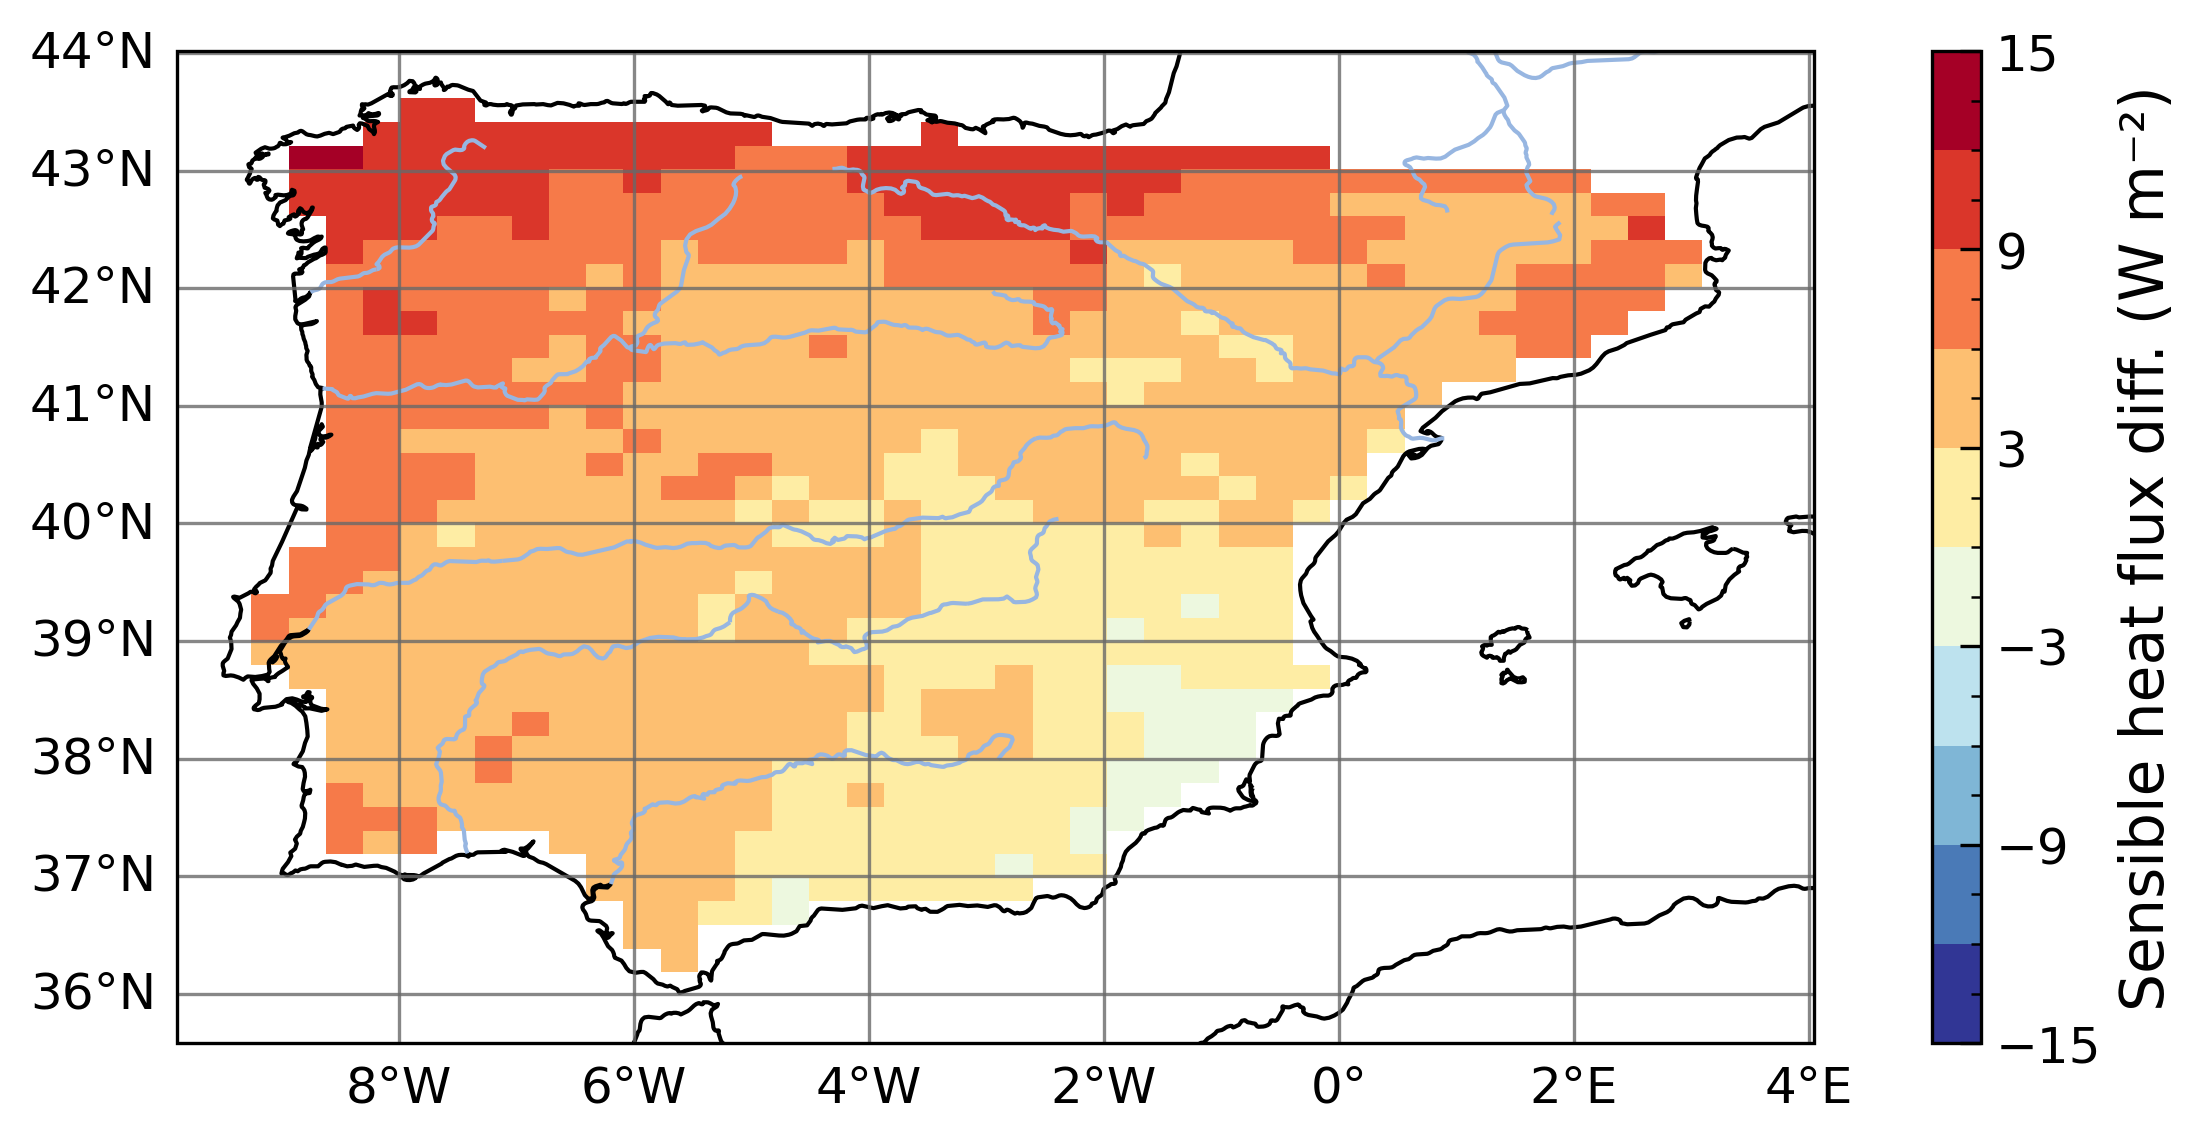
\includegraphics[width=\textwidth]{images/chap4/future/diffmap_fluxsens_presfut.png}
        \end{subfigure} \\
        
        %precip
        \begin{subfigure}[b]{0.5\textwidth}
            \caption{Precipitation difference}
            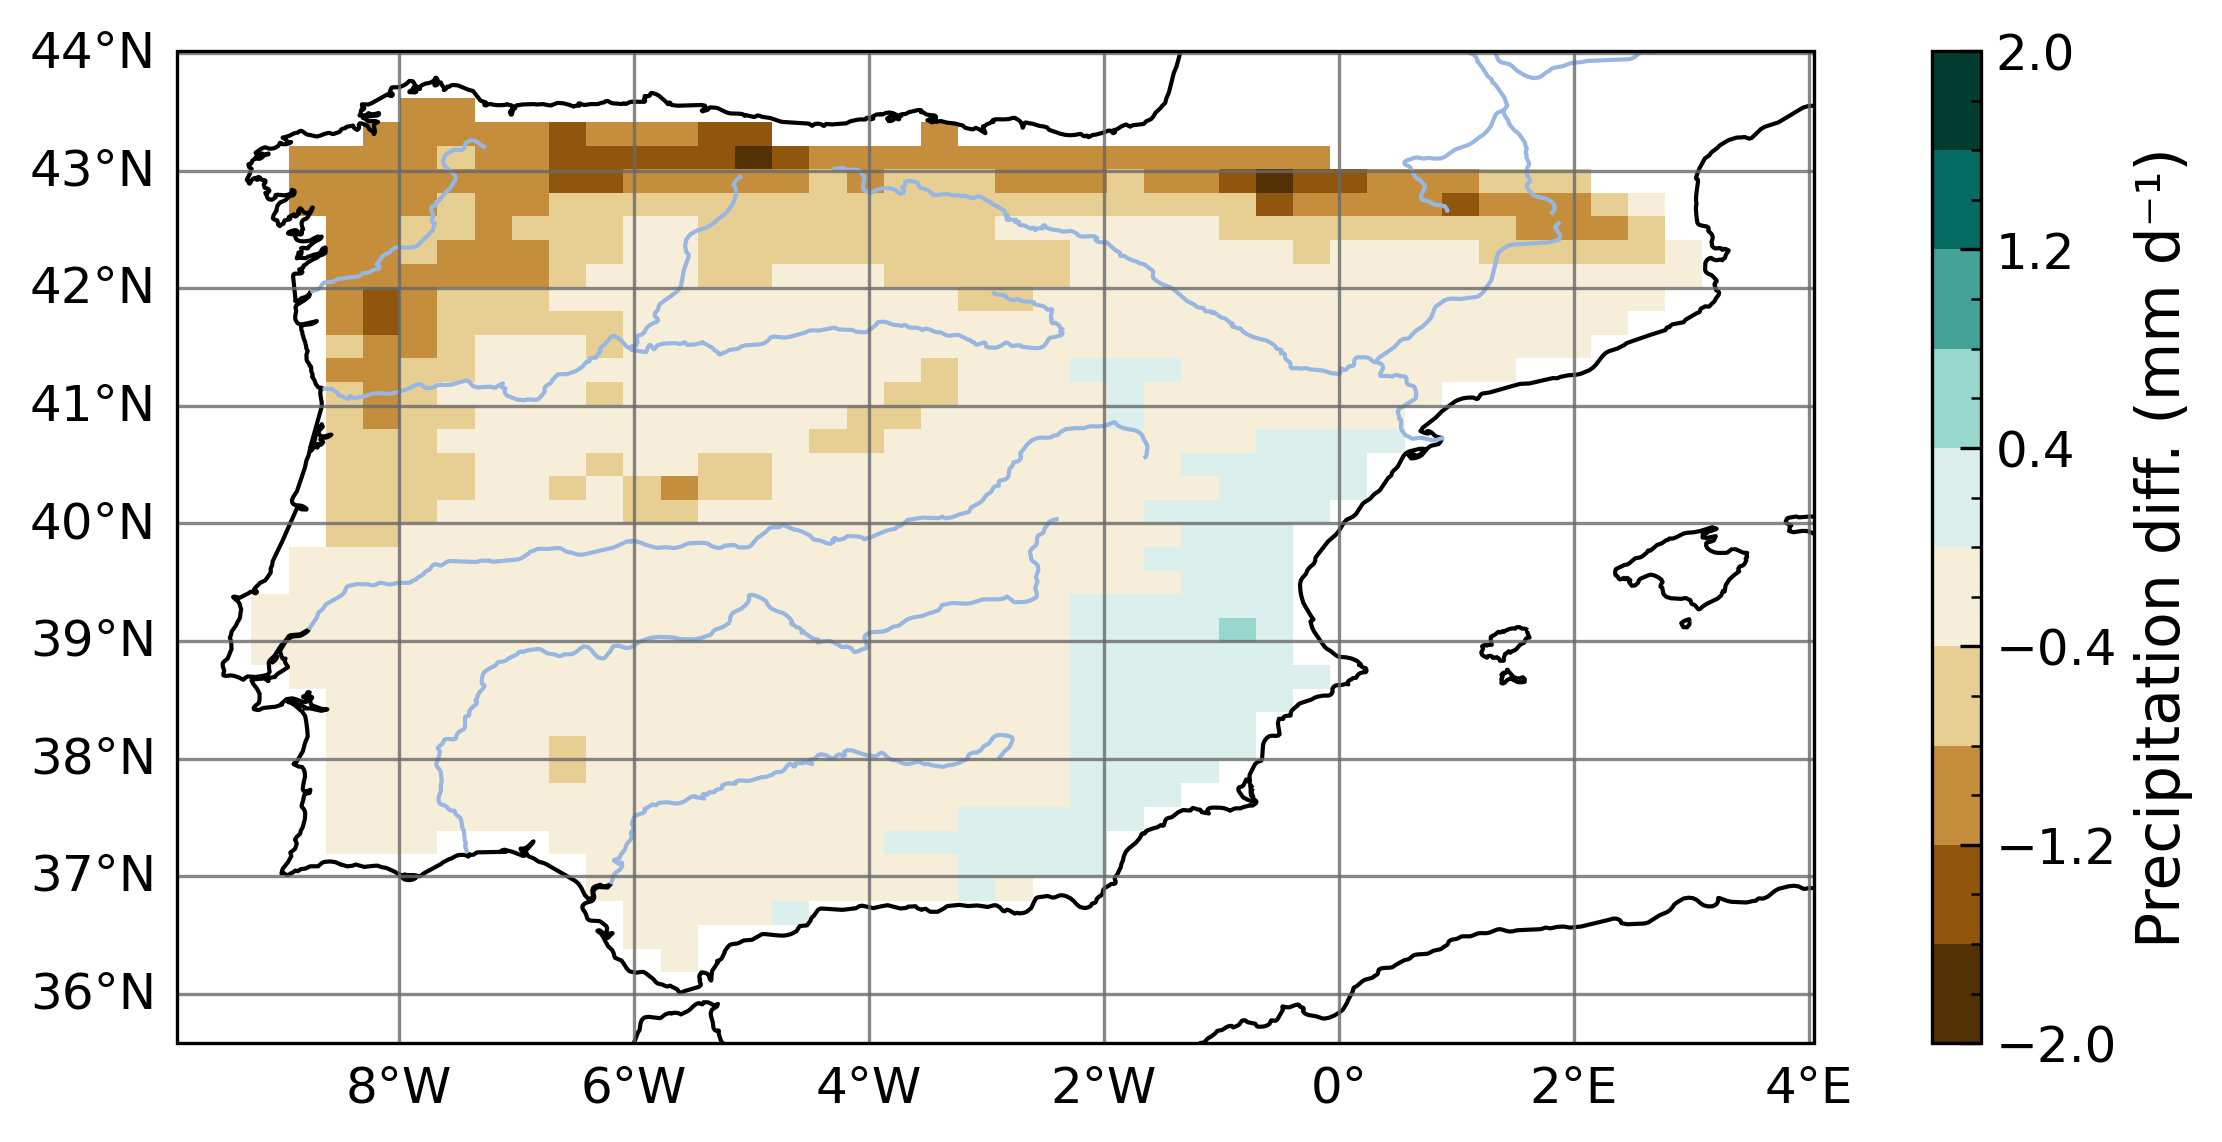
\includegraphics[width=\textwidth]{images/chap4/future/diffmap_precip_presfut.png}
        \end{subfigure} &
        %evap
        \begin{subfigure}[b]{0.5\textwidth}
            \caption{ET difference}
            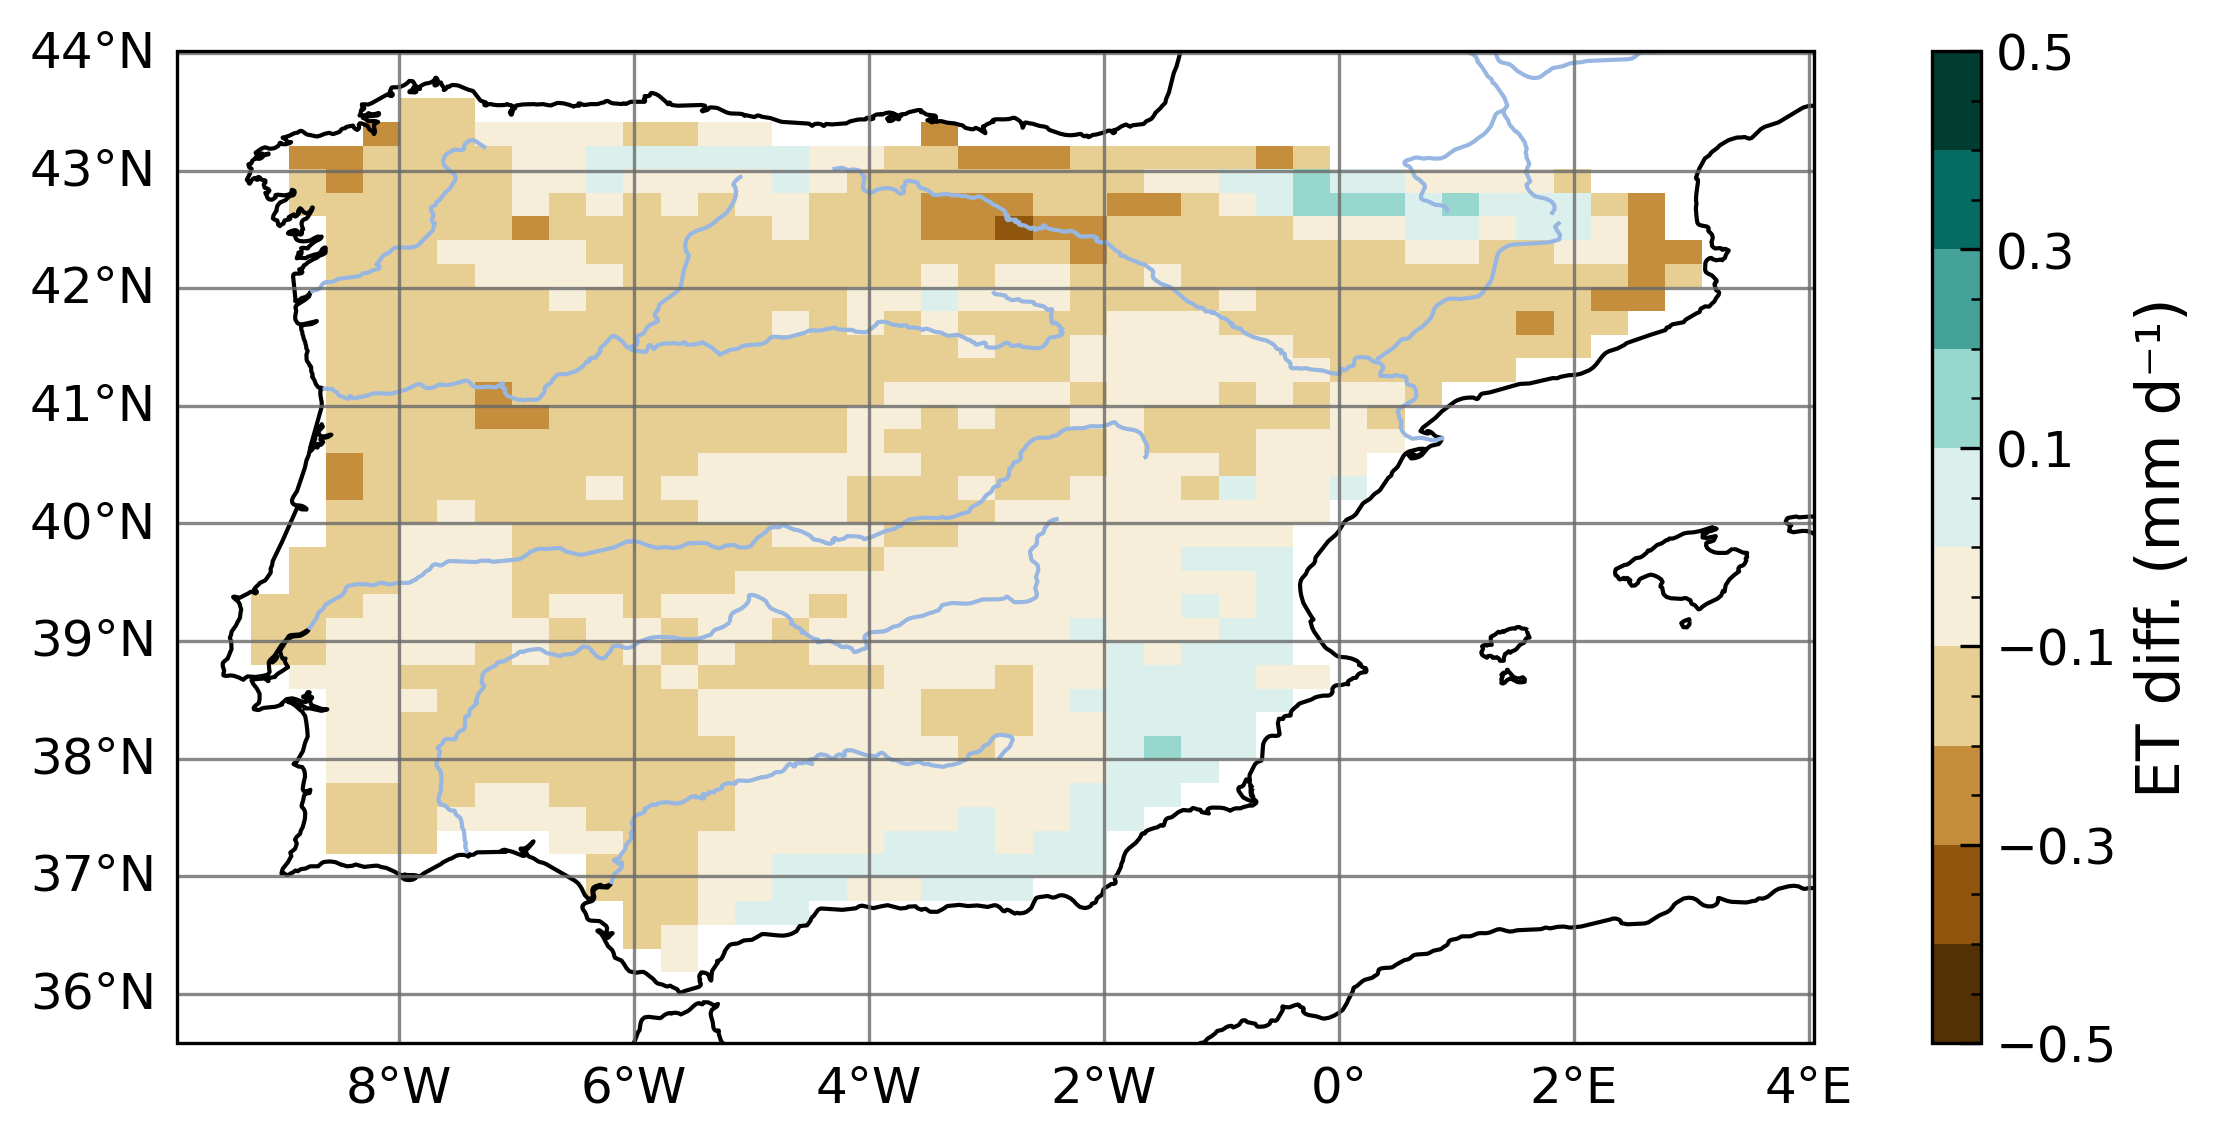
\includegraphics[width=\textwidth]{images/chap4/future/diffmap_evap_presfut.png}
        \end{subfigure} \\


        %q2m
        \begin{subfigure}[b]{0.5\textwidth}
            \caption{2-m specific humidity difference}
            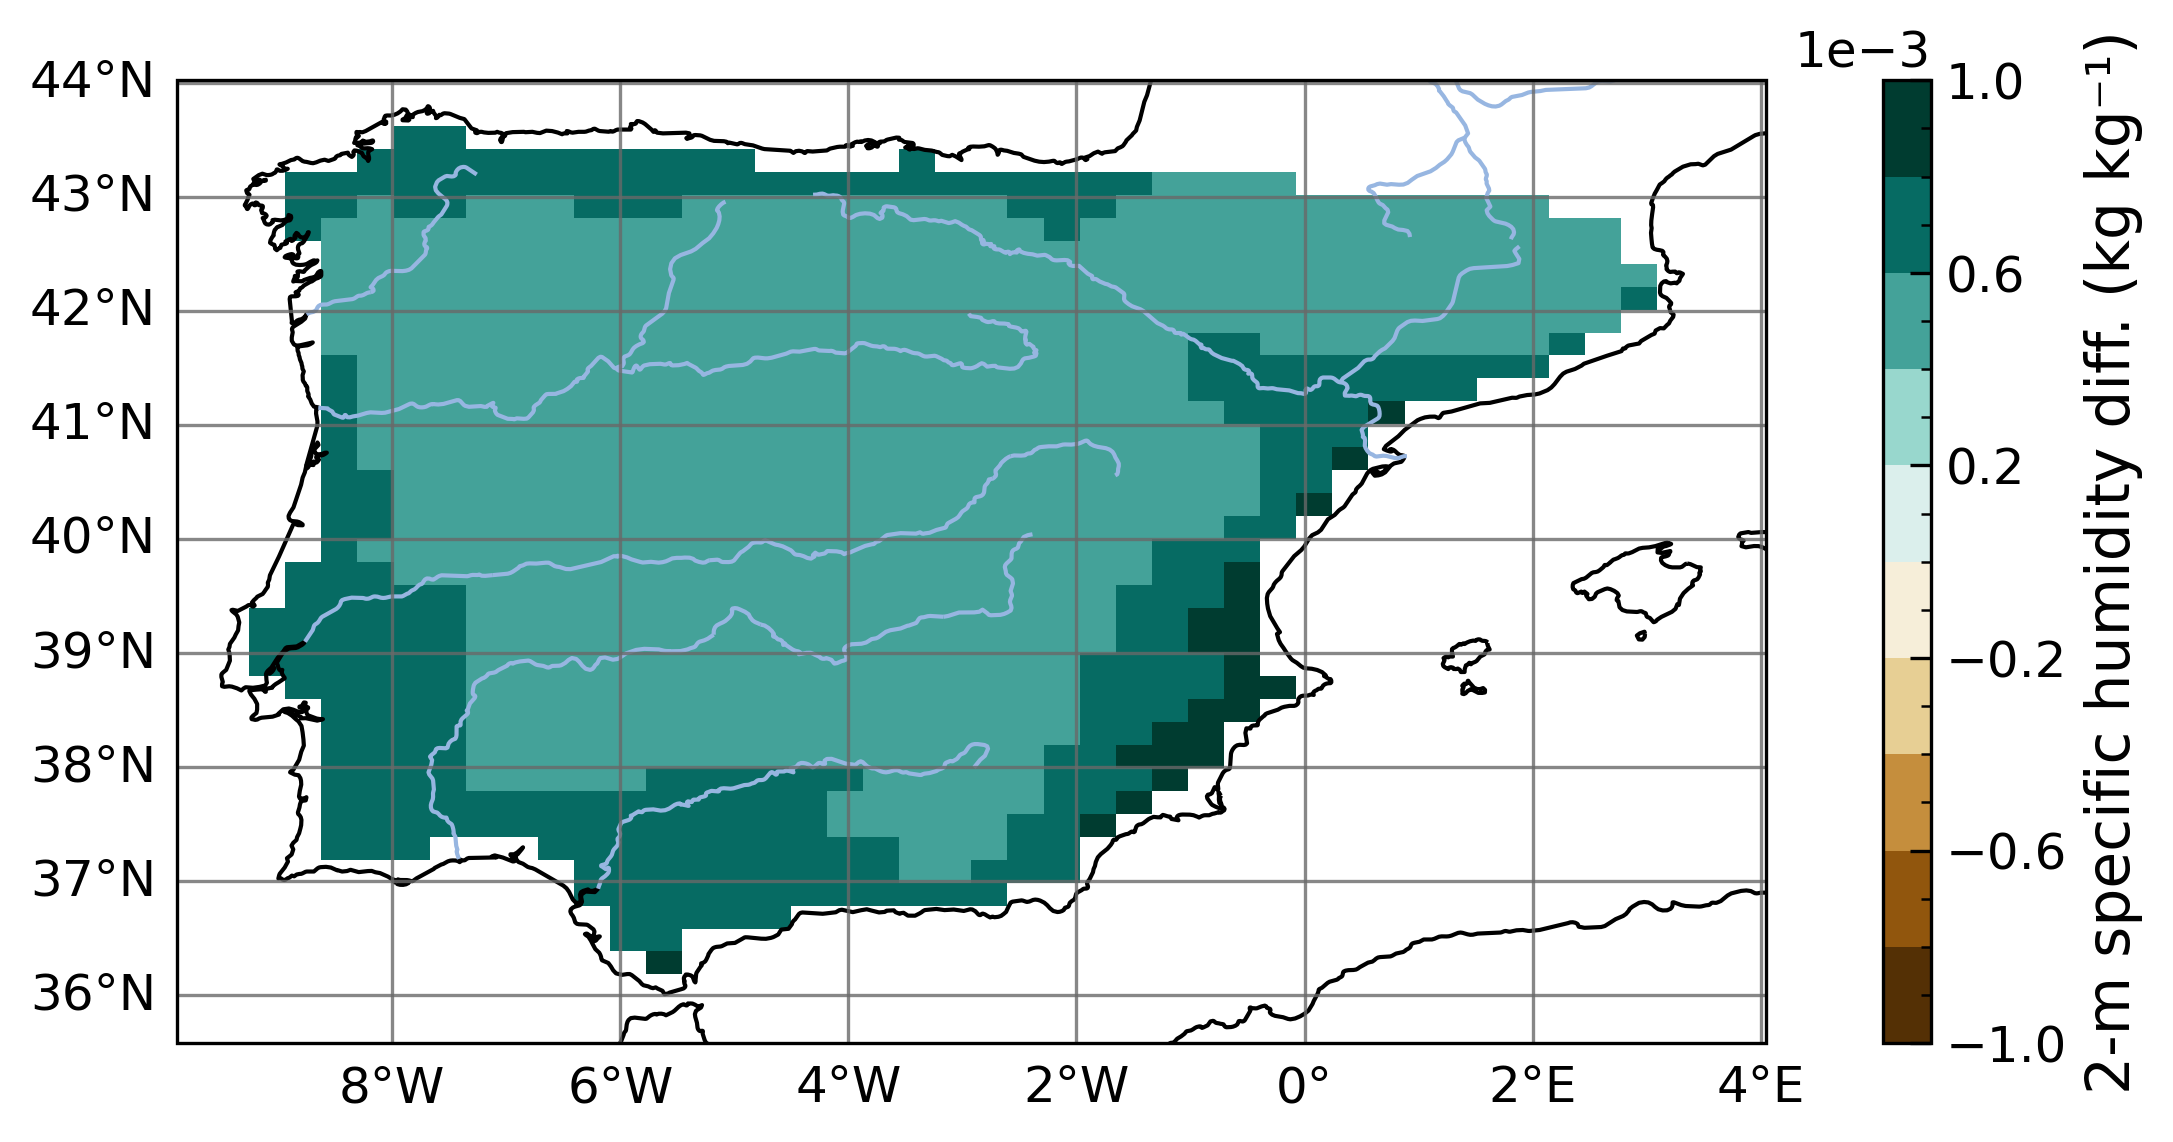
\includegraphics[width=\textwidth]{images/chap4/future/diffmap_q2m_presfut.png}
        \end{subfigure} &
        %rh2m
        \begin{subfigure}[b]{0.5\textwidth}
            \caption{2-m relative humidity difference}
            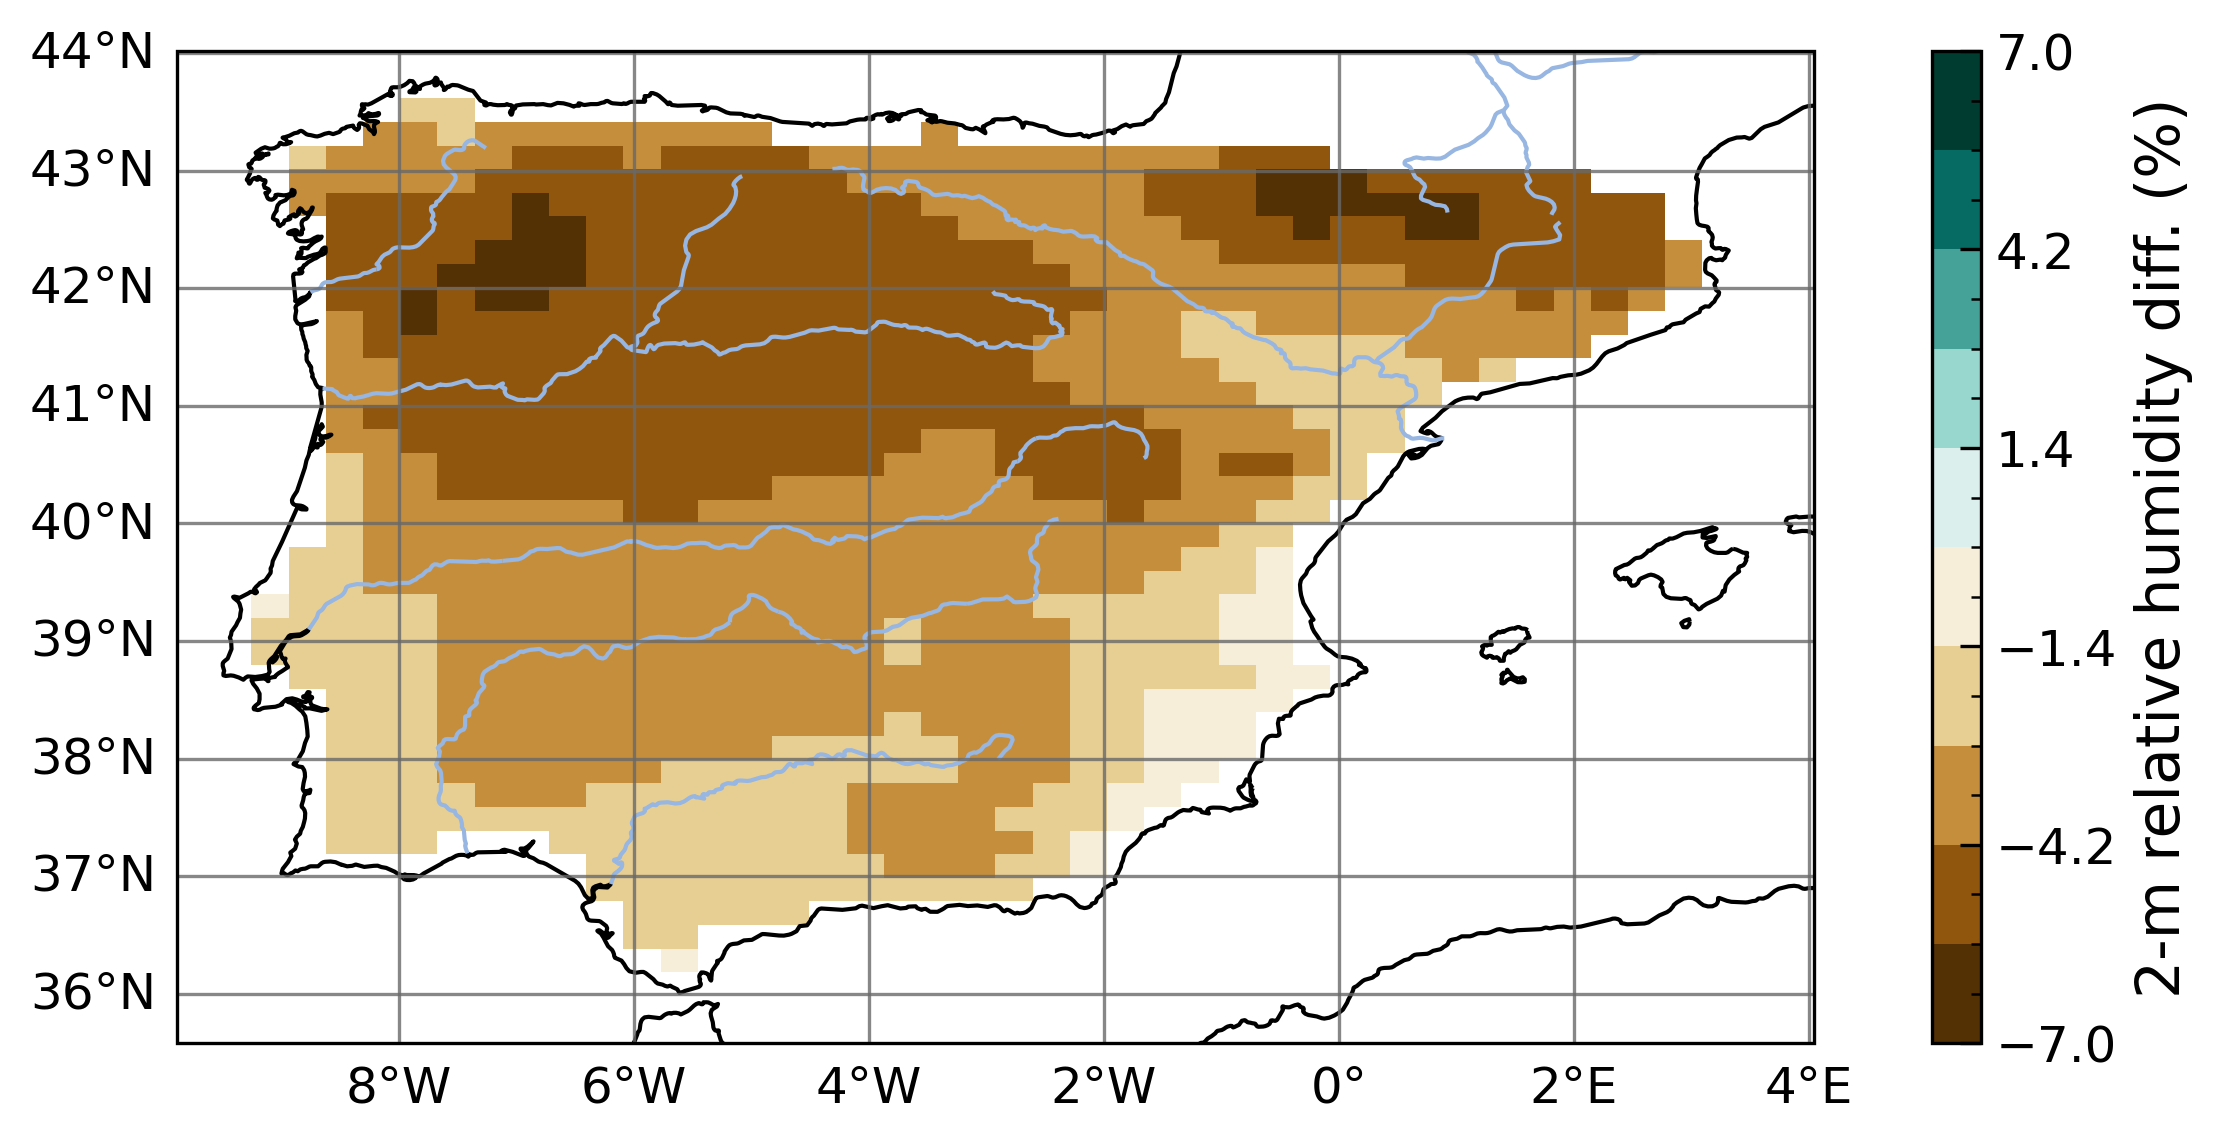
\includegraphics[width=\textwidth]{images/chap4/future/diffmap_rh2m_presfut.png}
        \end{subfigure} \\

        %SWdnSFC
        \begin{subfigure}[b]{0.5\textwidth}
            \caption{Downwelling shortwave radiation difference}
            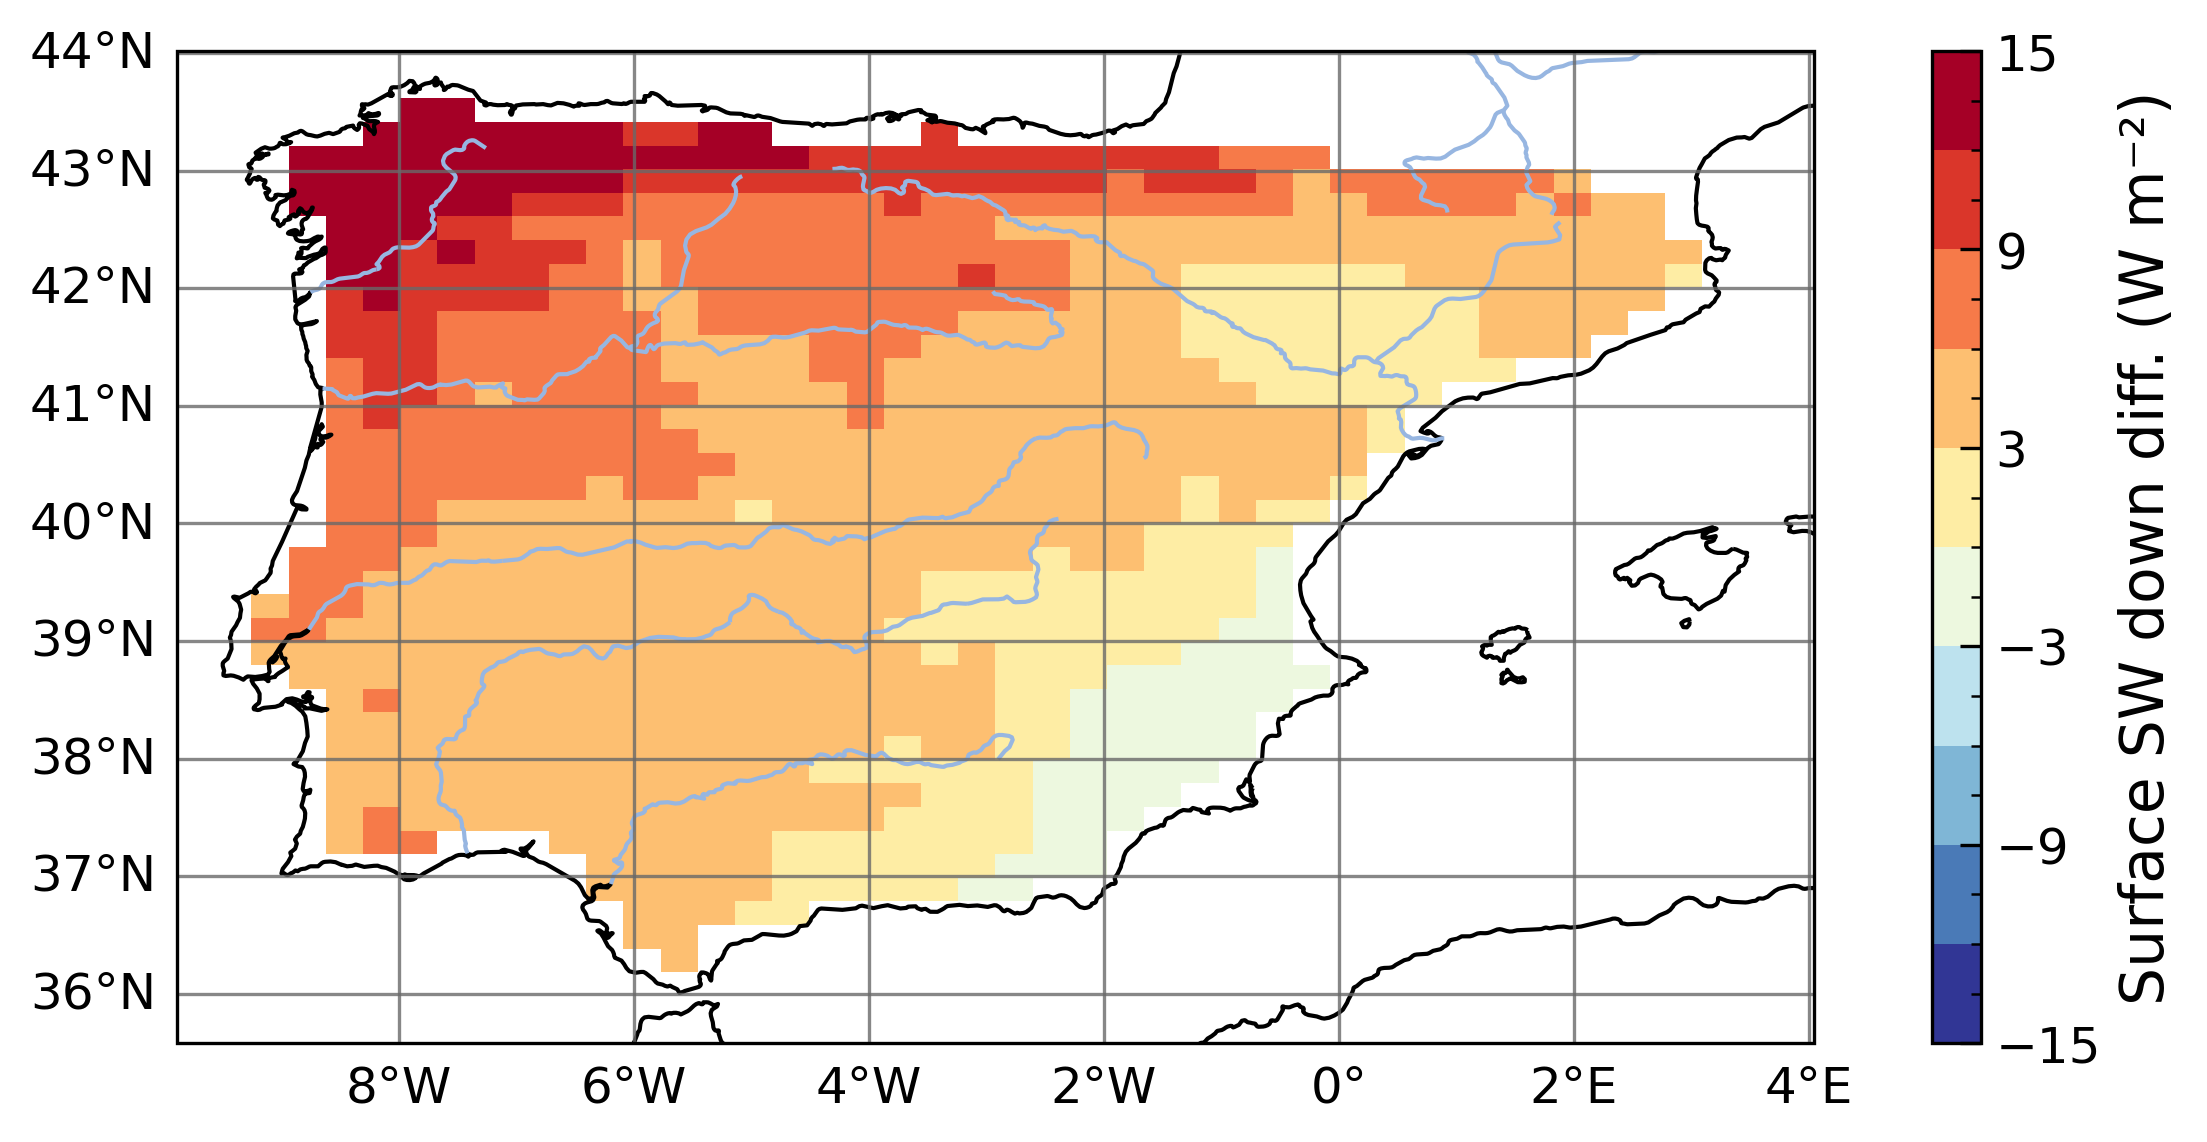
\includegraphics[width=\textwidth]{images/chap4/future/diffmap_SWdnSFC_presfut.png}
        \end{subfigure} &
        %LWdnSFC
        \begin{subfigure}[b]{0.5\textwidth}
            \caption{Downwelling longwave radiation difference}
            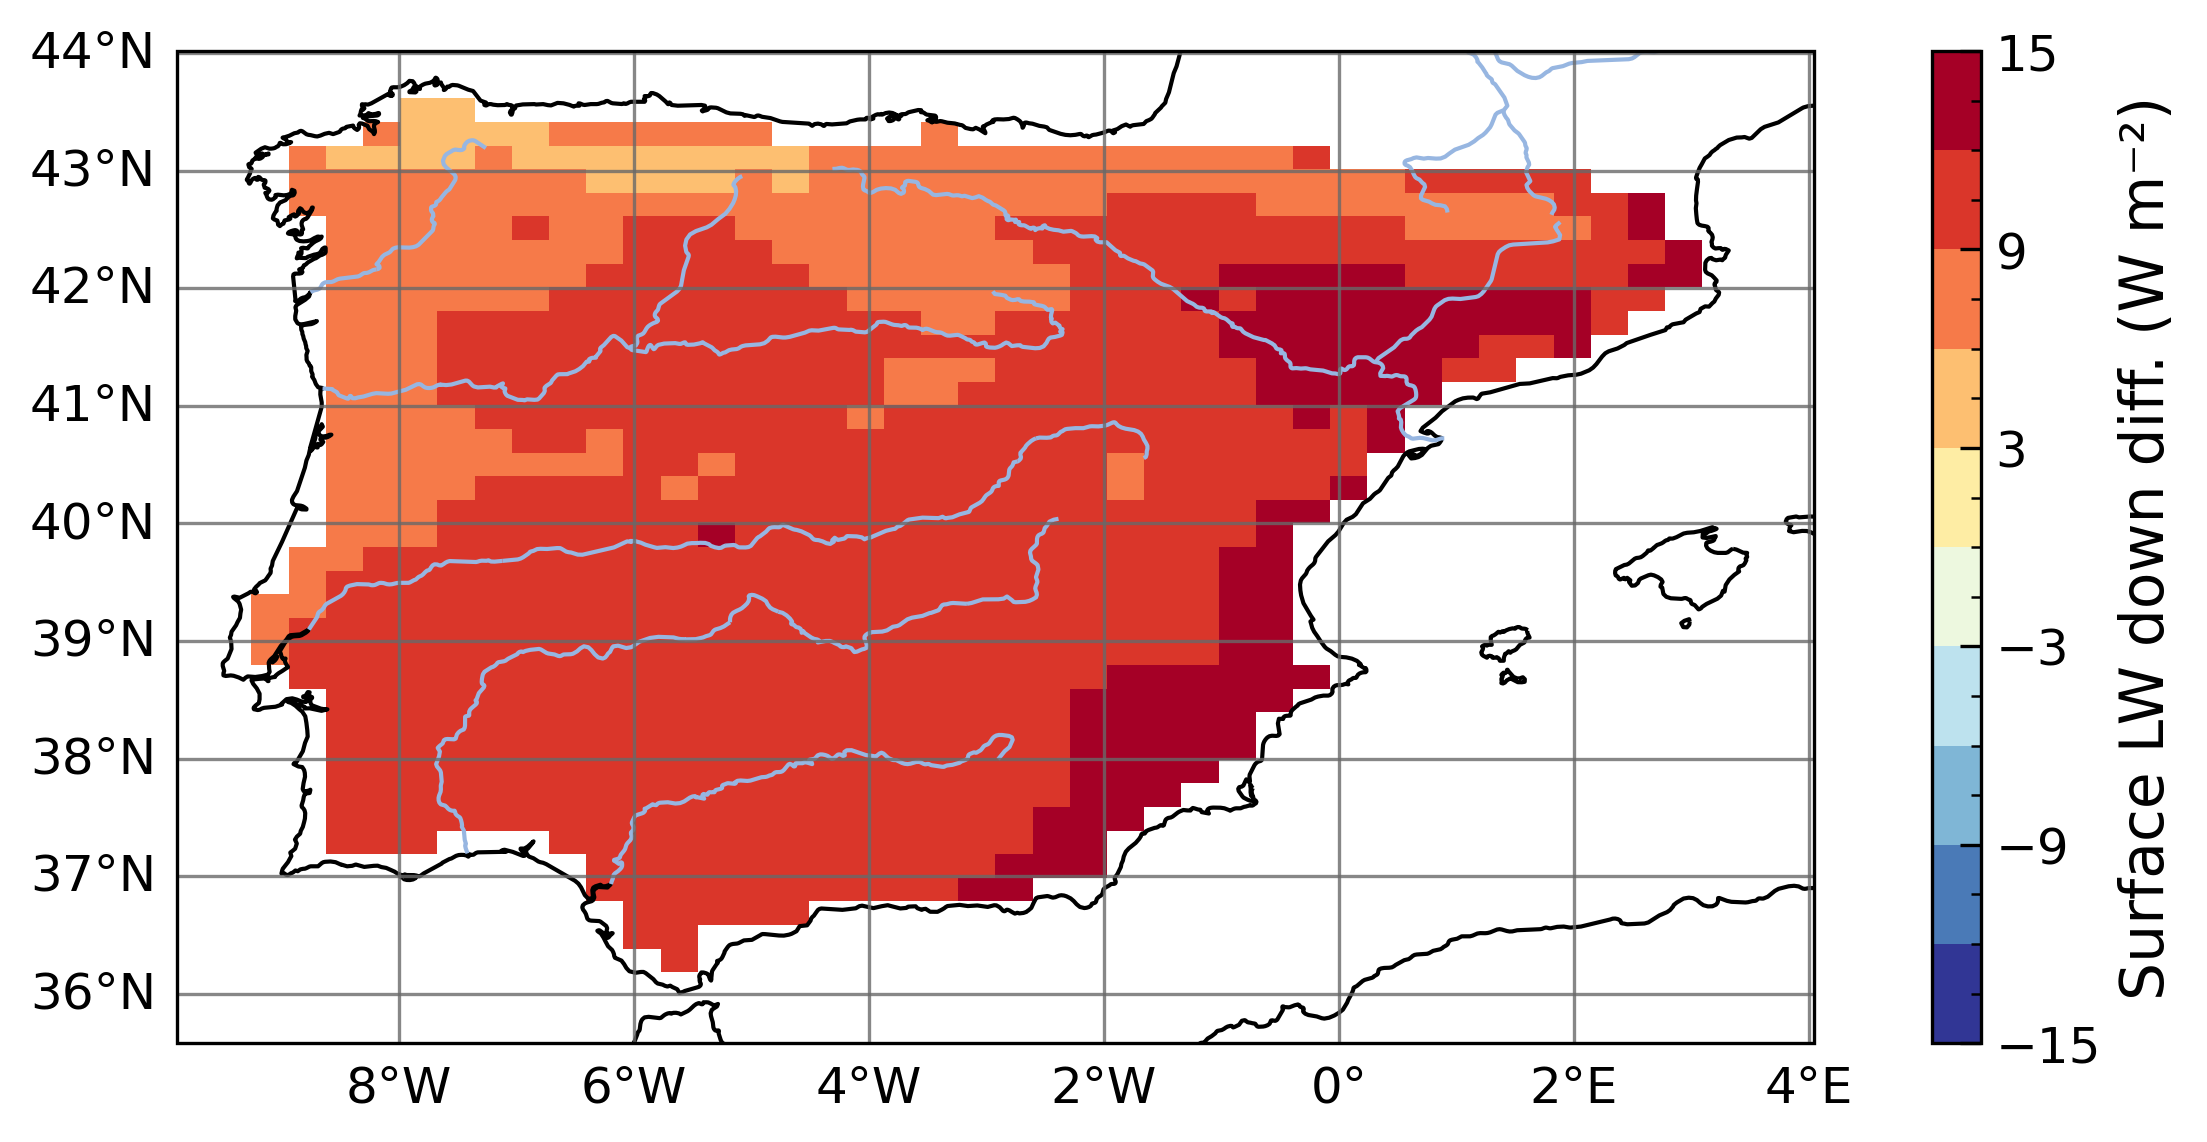
\includegraphics[width=\textwidth]{images/chap4/future/diffmap_LWdnSFC_presfut.png}
        \end{subfigure}
    \end{tabular}
    \caption{Impacts of climate change over the Iberian Peninsula. Annual mean difference between \futnoirr (2050-2062) and  \presnoirr (2010-2022).}
    \label{fig:diffmaps_present_future}
\end{figure}

\clearpage

\subsection{Impacts of irrigation under climate change}
%todo: FC Est ce que tu peux comparer  l'intensité du recyclage induit par l irrigation, local et remote, en climat modifié à celui analysé pour le climat récent? 

%figure : map and SC of irrigation in the future
\begin{figure}[htbp]
    \centering
    \begin{tabular}{cc}
        %precip
        \begin{subfigure}[b]{0.48\textwidth}
            \caption{Irrigation annual mean}
            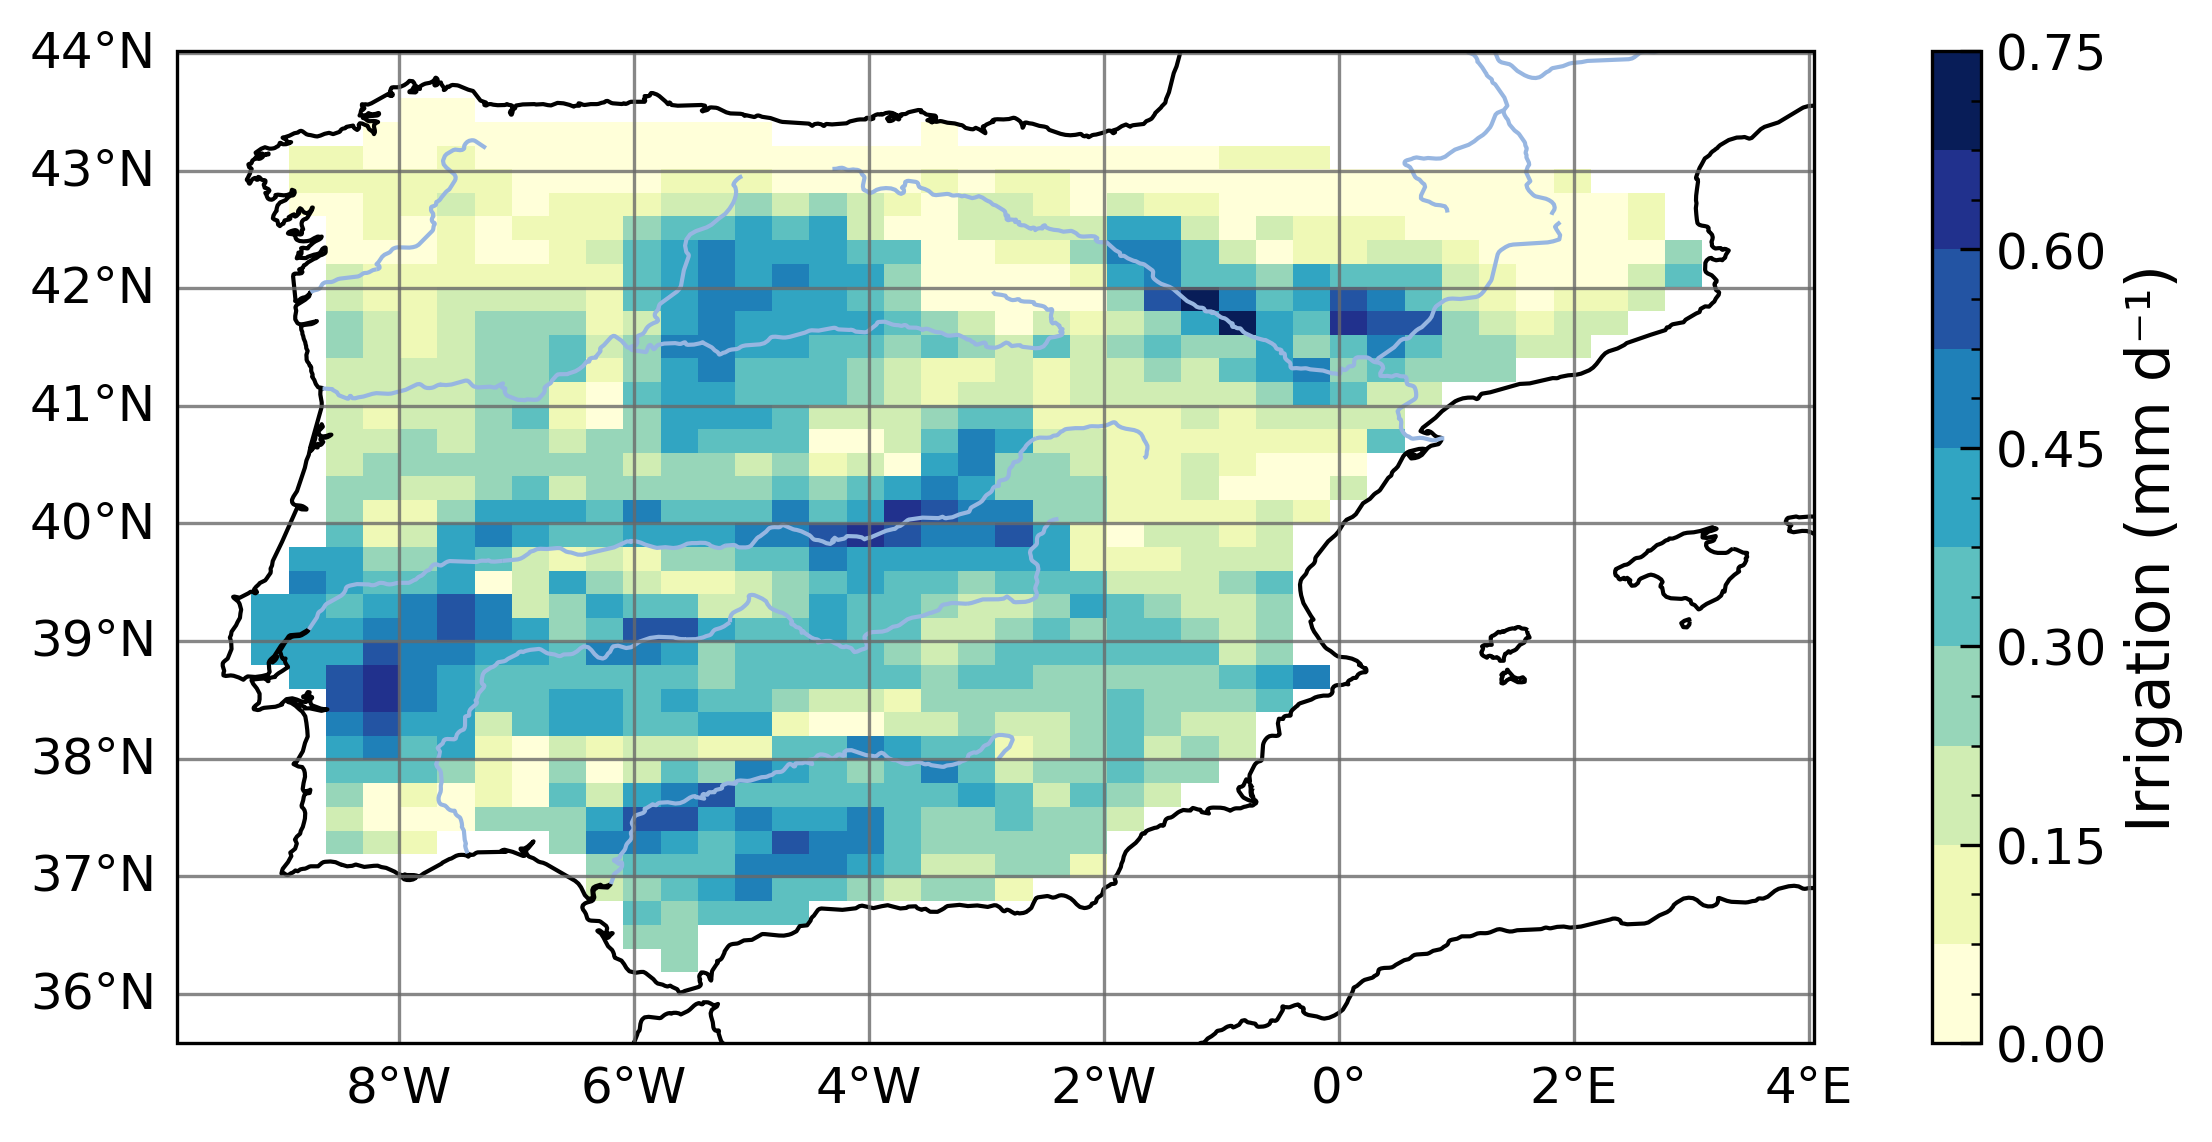
\includegraphics[width=\textwidth]{images/chap4/future/map_irrigation_fut.png}
        \end{subfigure} &
        \begin{subfigure}[b]{0.46\textwidth}
            \caption{Irrigation mean seasonal cycle}
            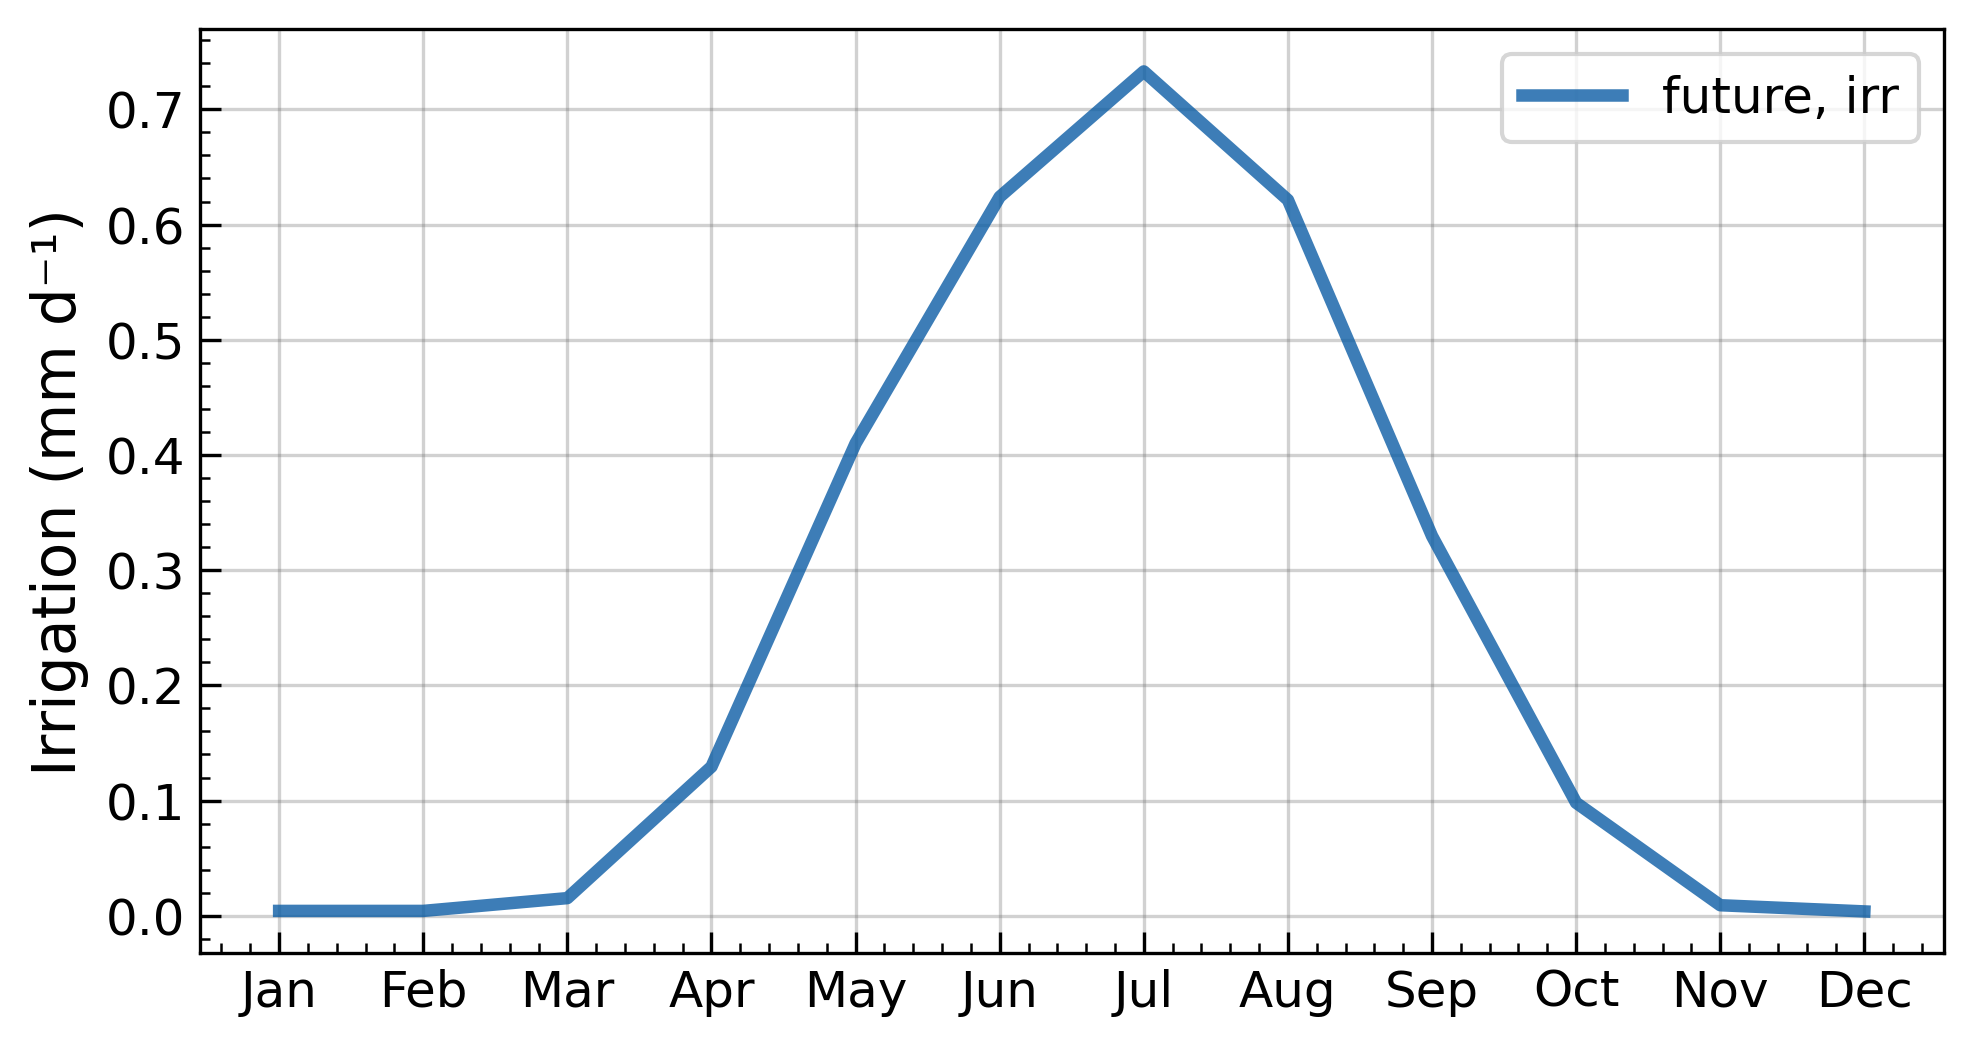
\includegraphics[width=\textwidth]{images/chap4/future/SC_irrigation_fut.png}
        \end{subfigure}
    \end{tabular}
    \caption{Annual mean and seasonal cycle of irrigation over the Iberian Peninsula in the \futirr simulation (2050-2062).}
    \label{fig:future_irrig}
\end{figure}

Irrigation in the \futirr simulation is largest in the valleys of the Ebro, Douro, Tagus, Guadiana and Guadalquivir rivers (Fig. \ref{fig:future_irrig}a). Due to modelling choices, it is near-zero in winter, and follows a rather symmetrical seasonal cycle from spring to autumn, with a peak in July (Fig. \ref{fig:future_irrig}b).
It is important to note that this simulation cannot be directly compared to the simulation of irrigation in present condition presented in Section \ref{sec:article1}, for two reasons. First, the simulation setup is different since a smaller domain with lateral boundary conditions from ICOLMDZOR are used, instead of the intermediate domain and ERA5 data. Secondly, a technical issue with the routing scheme occurred when running this simulation with irrigation under future climate. A different setting was inappropriately used, which alters the routing scheme parameters determined in Chapter \ref{chap:routing}, dividing them by 1000. This leads to irrelevant values for river discharge (not shown here) and very large volumes of water available in the routing reservoirs. In practice, that means that irrigation was mostly not constrained by available water in this simulation, and that irrigation demand was systematically met, maintaining soil moisture at 60\% of field capacity in irrigated areas.
To some extent, this setup can be considered as a sensitivity experiment representing a situation where irrigation infrastructure can provide very large amounts of water. Also, this likely circumvents the limitations of the \textit{normal} irrigation scheme setup identified in Section \ref{sec:article1} for southern regions, where irrigation was highly underestimated. Therefore, this simulation was still used for a preliminary study of atmospheric feedbacks of irrigation.

%turbulent fluxes
Compared to the \futnoirr simulation, the most direct impact of irrigation is an increase in ET of similar amplitude to the irrigation amounts (Fig. \ref{fig:diffmaps_future_irr}d), which largely compensates for the decrease in ET induced by climate change. This increase of the latent heat flux is directly linked to a decrease of the sensible heat flux (Fig. \ref{fig:diffmaps_future_irr}b) reaching -15 W \persqm in the most irrigated valleys. 
%t2m
This new partitioning of surface energy leads to a cooler air over most of the domain (Fig. \ref{fig:diffmaps_future_irr}a). The largest decreases occur  over the intensely irrigated areas where 2-meter temperature is lowered by 0.5°C on annual average and 1°C in summer (see appendix Fig. \ref{fig:diffmaps_JJA_future_irr} for JJA impacts). 
Contrary to ET, this consequence of irrigation is insufficient to compensate the impact of climate change, which induces 2-meter temperature increases of 2°C annually and larger than 3°C in summer.
Regarding humidity, \futirr is moister than \futnoirr (Fig. \ref{fig:diffmaps_future_irr}e) but some intensely irrigated areas such as the Ebro valley show smaller increases in specific humidity than others, showing that the impacts on humidity are not a local as those on temperature. Combined with the changes in temperature, the increase of specific humidity also leads to an increase in relative humidity  (Fig. \ref{fig:diffmaps_future_irr}f), which opposes the impact of climate change, without reverting it.
%ABL
The structure of the boundary layer is also affected by irrigation, as seen in Section \ref{sec:article1}. Stabilization dominates and follows the same pattern as irrigation, as a consequence of cooling and of the reduced sensible heat flux. The ABL height is lowered by more than a 100 m in the most intensely irrigated grid cells. 
Due to the moistening and cooling of the atmosphere, the lifting condensation level is also lowered. Similarly to the changes in 2-meter humidity, LCL is more affected in the Tagus, Guadiana and Guadalquivir basins than in the Ebro and Douro basins.
As explained in Section \ref{sec:article1}, the lowering of both the ABL height and LCL point to opposite effects on cloud formation and precipitation, since one reflects a more stable atmosphere less likely to form clouds through convection, while the other is associated with a moister and cooler atmosphere where condensation is more likely. As a consequence, the impact of irrigation on precipitation is rather limited and the only structures that emerge are precipitation increases in the highest mountain ranges (the Betic, Central, Iberian Systems and the Pyrenees), and a decrease in the northern Ebro valley (more clearly visible by looking at relative changes in Fig. \ref{fig:reldiffmaps_future_irr}c).

%figure : diff maps (future, irr - no_irr)
\begin{figure}[htbp]
    \centering
    \begin{tabular}{cc}
        %t2m
        \begin{subfigure}[b]{0.5\textwidth}
            \caption{2-m temperature difference}
            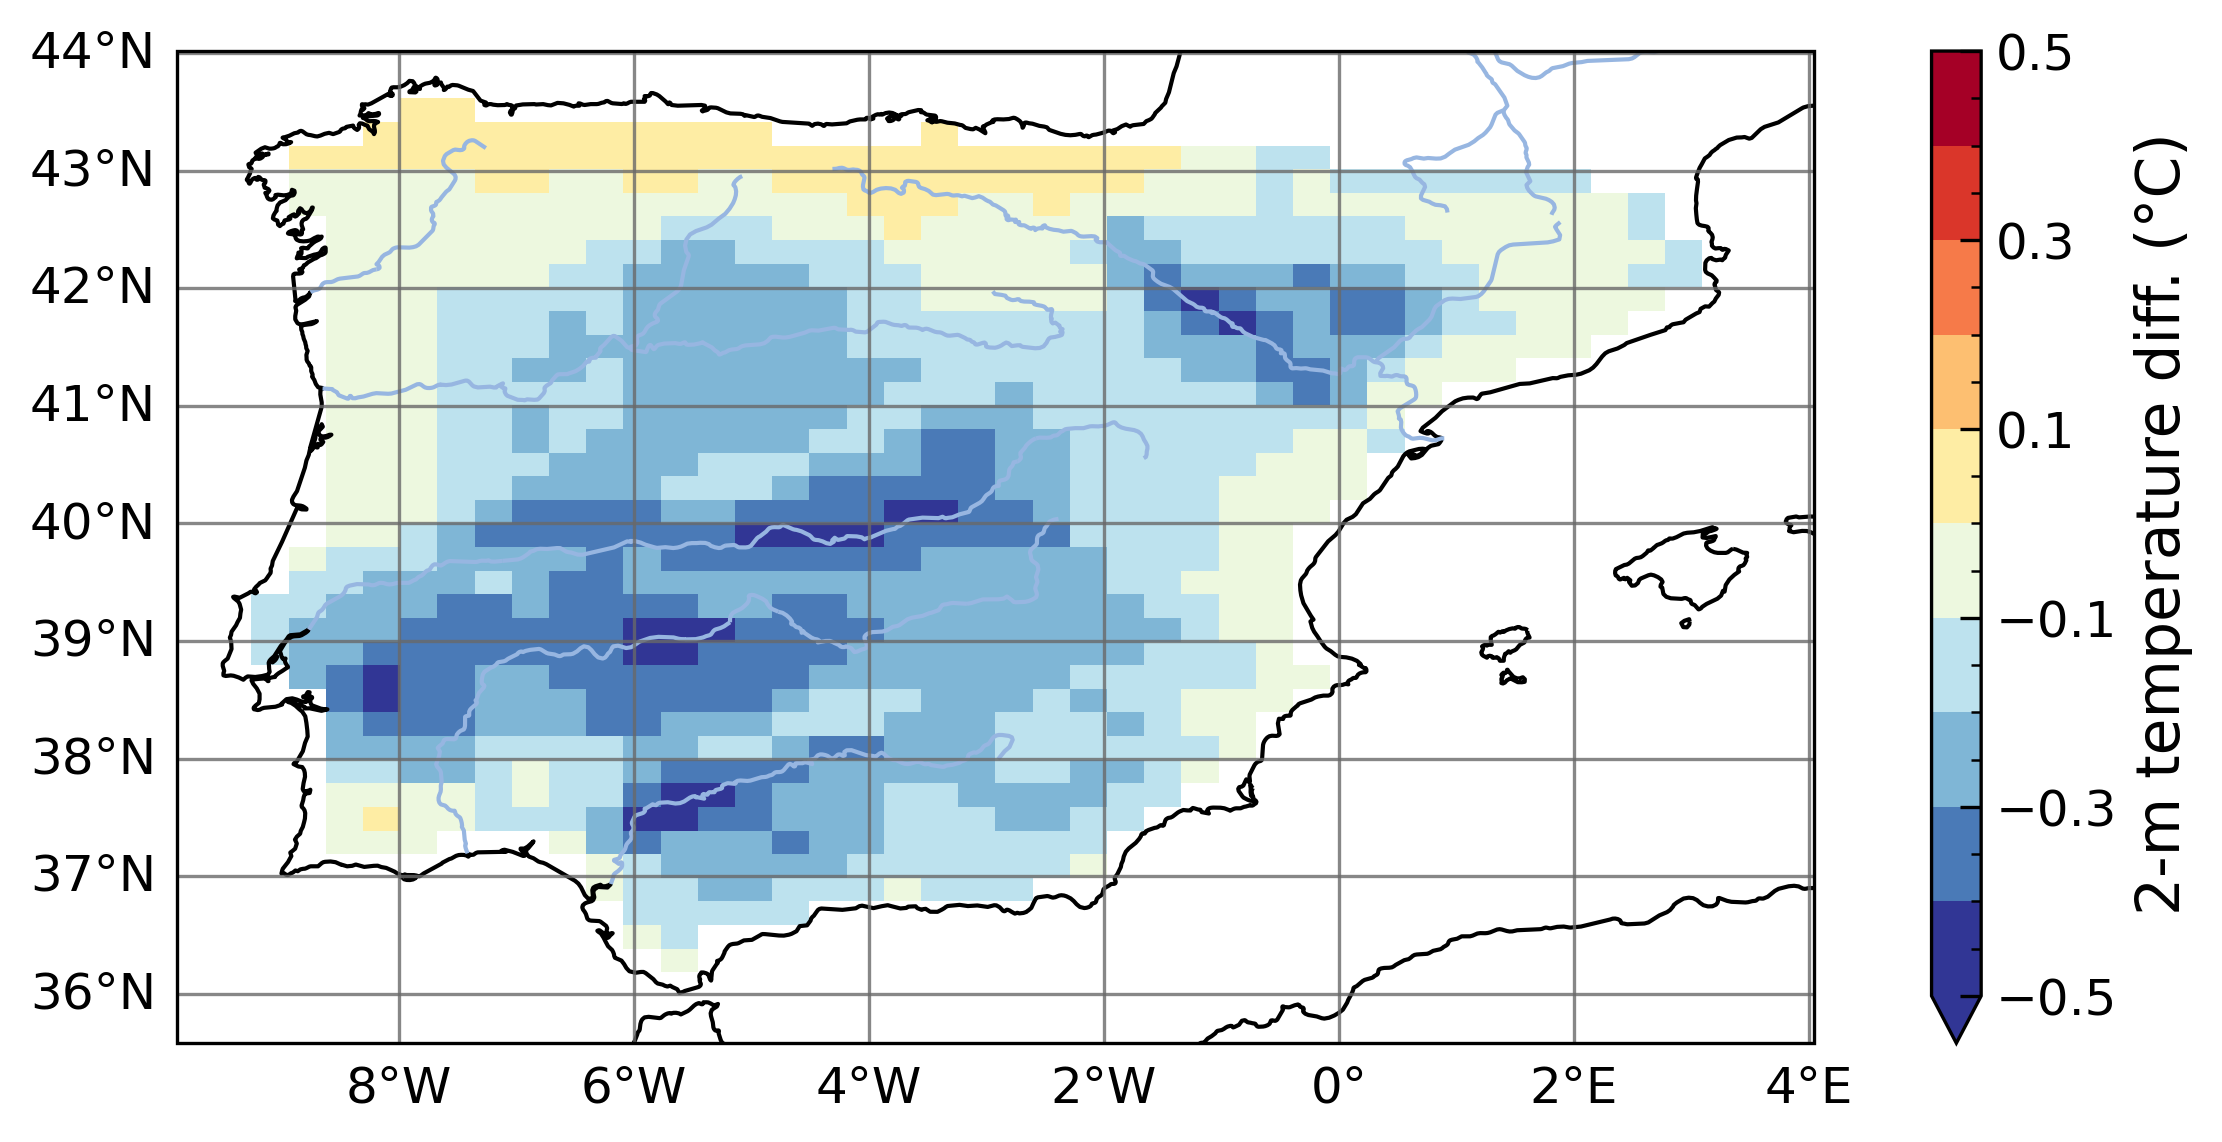
\includegraphics[width=\textwidth]{images/chap4/future/diffmap_t2m_futirr.png}
        \end{subfigure} &
        %fluxsens
        \begin{subfigure}[b]{0.5\textwidth}
            \caption{Sensible heat flux difference}
            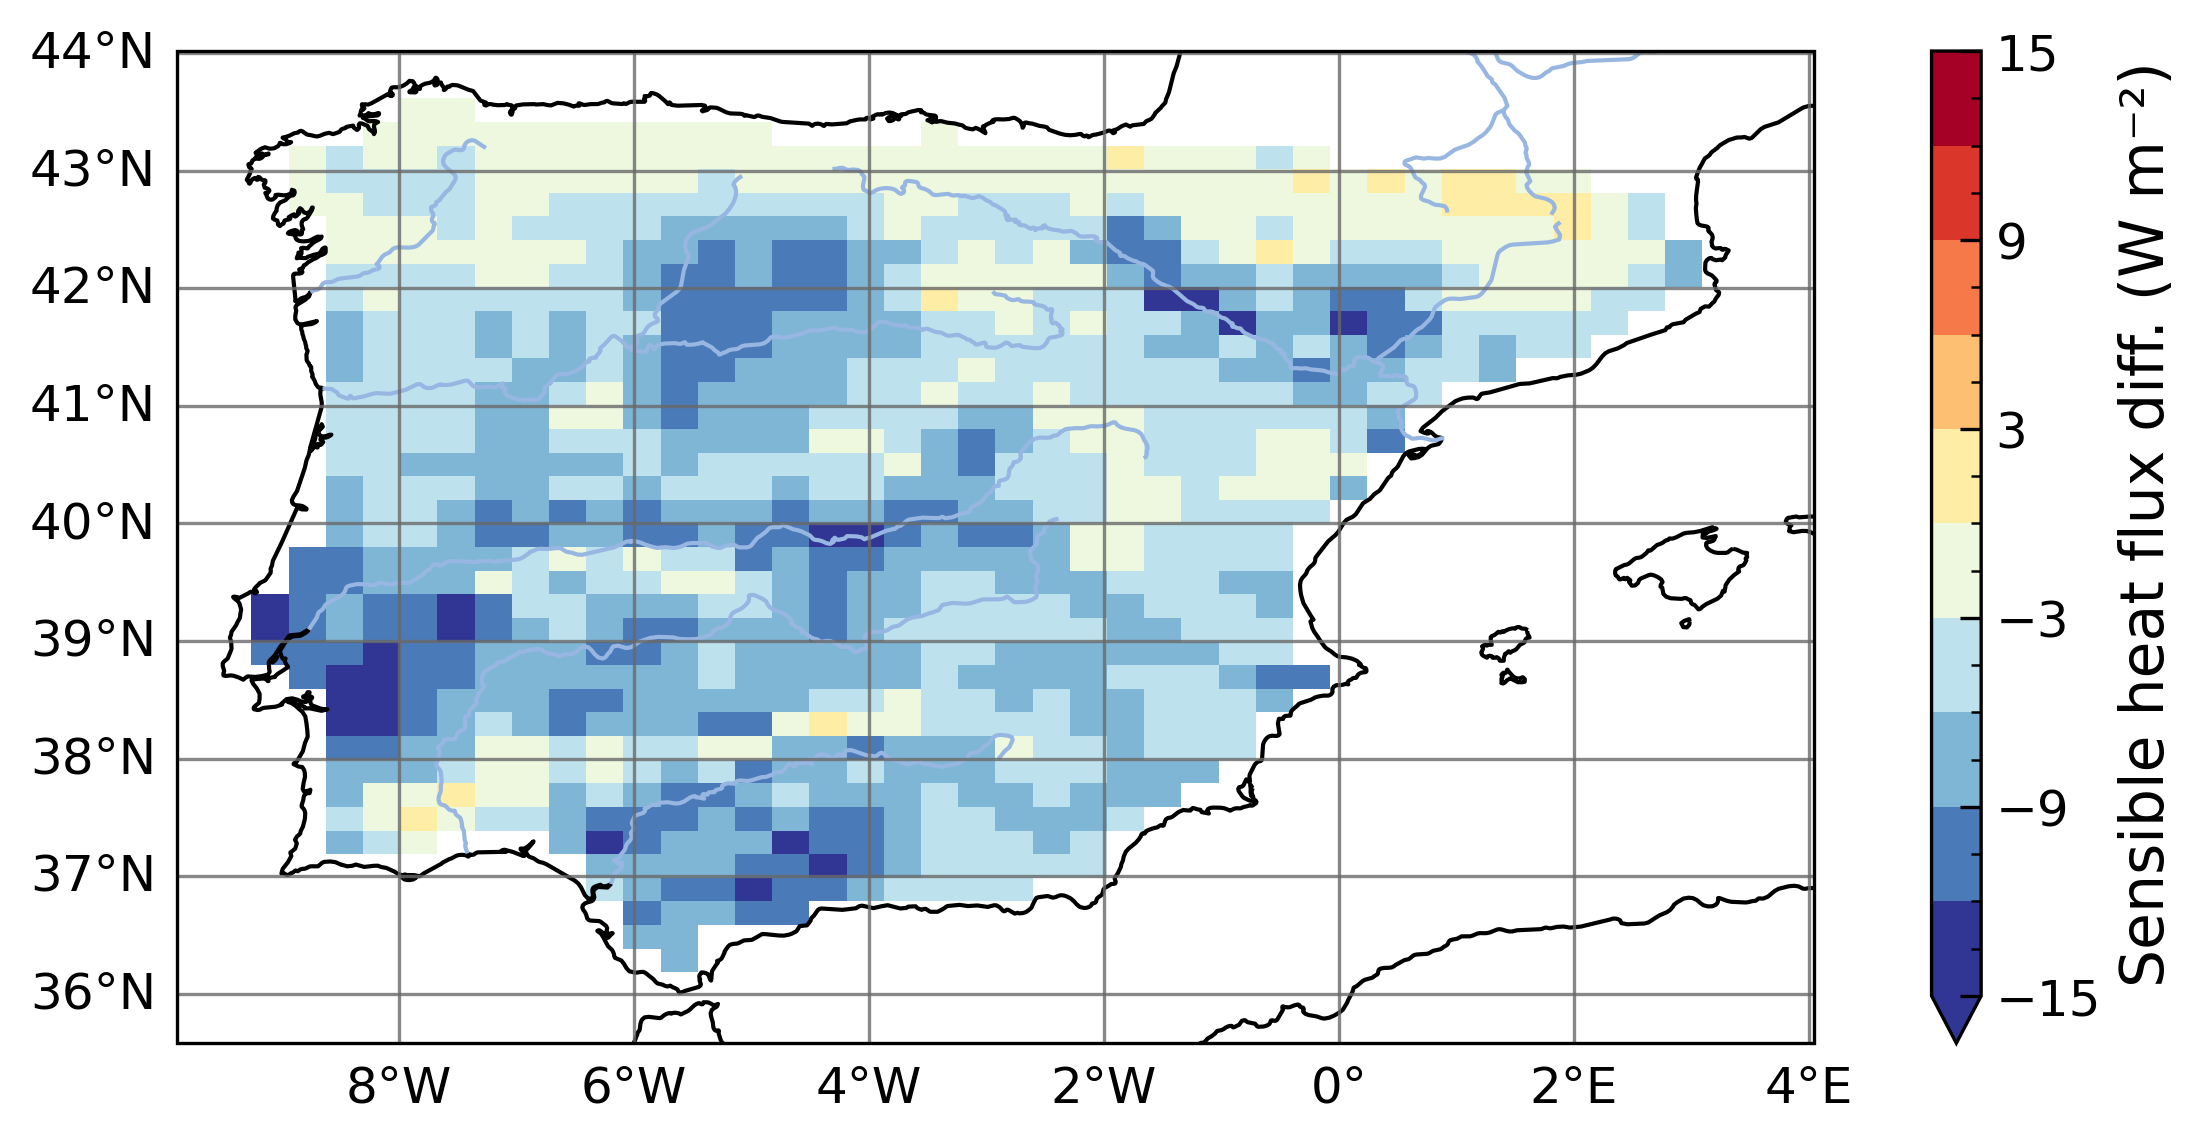
\includegraphics[width=\textwidth]{images/chap4/future/diffmap_fluxsens_futirr.png}
        \end{subfigure} \\

        %precip
        \begin{subfigure}[b]{0.5\textwidth}
            \caption{Precipitation difference}
            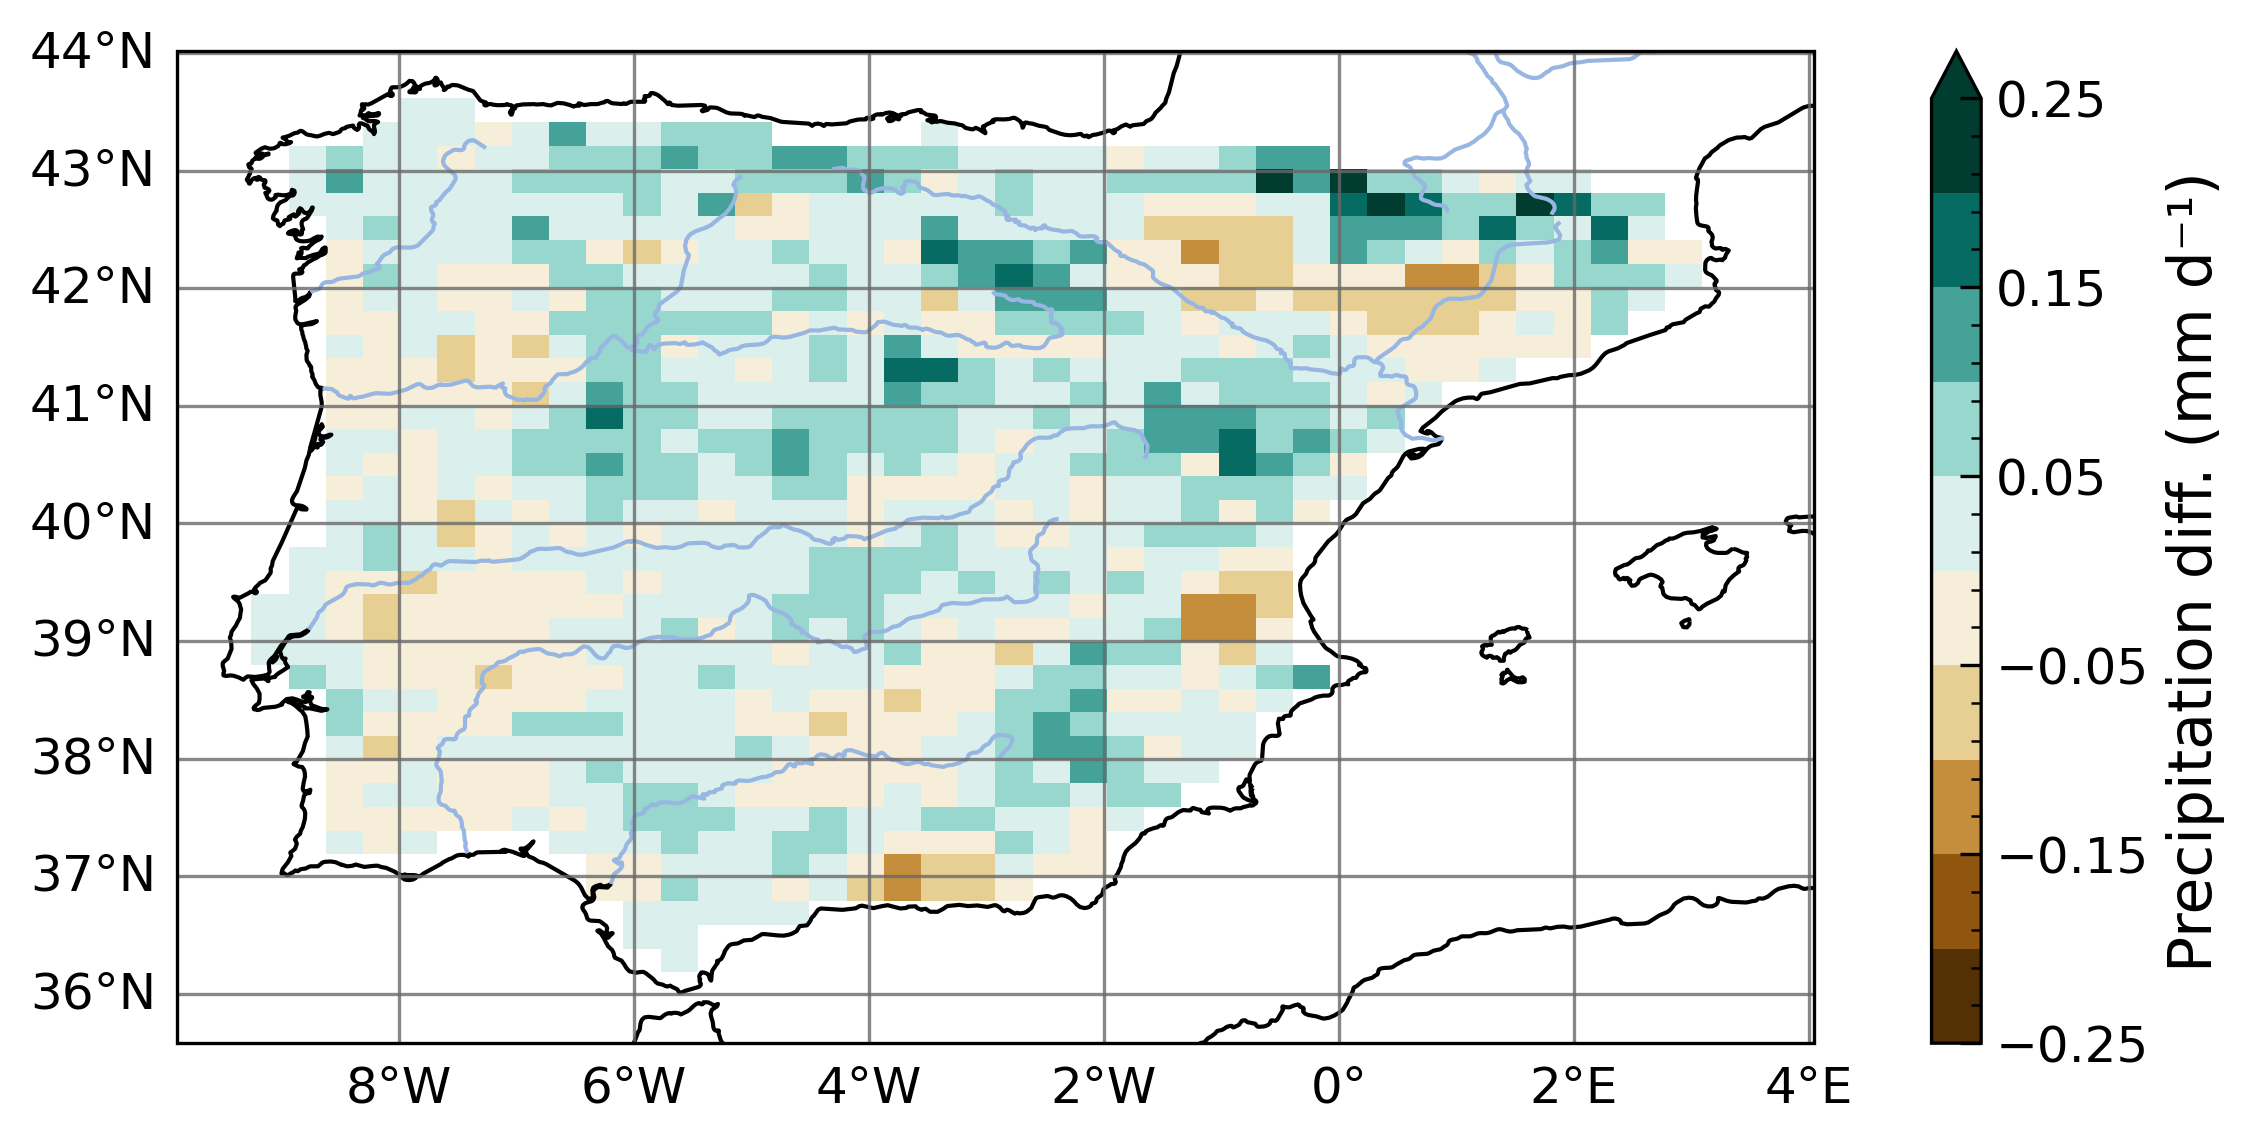
\includegraphics[width=\textwidth]{images/chap4/future/diffmap_precip_futirr.png}
        \end{subfigure} &
        %evap
        \begin{subfigure}[b]{0.5\textwidth}
            \caption{ET difference}
            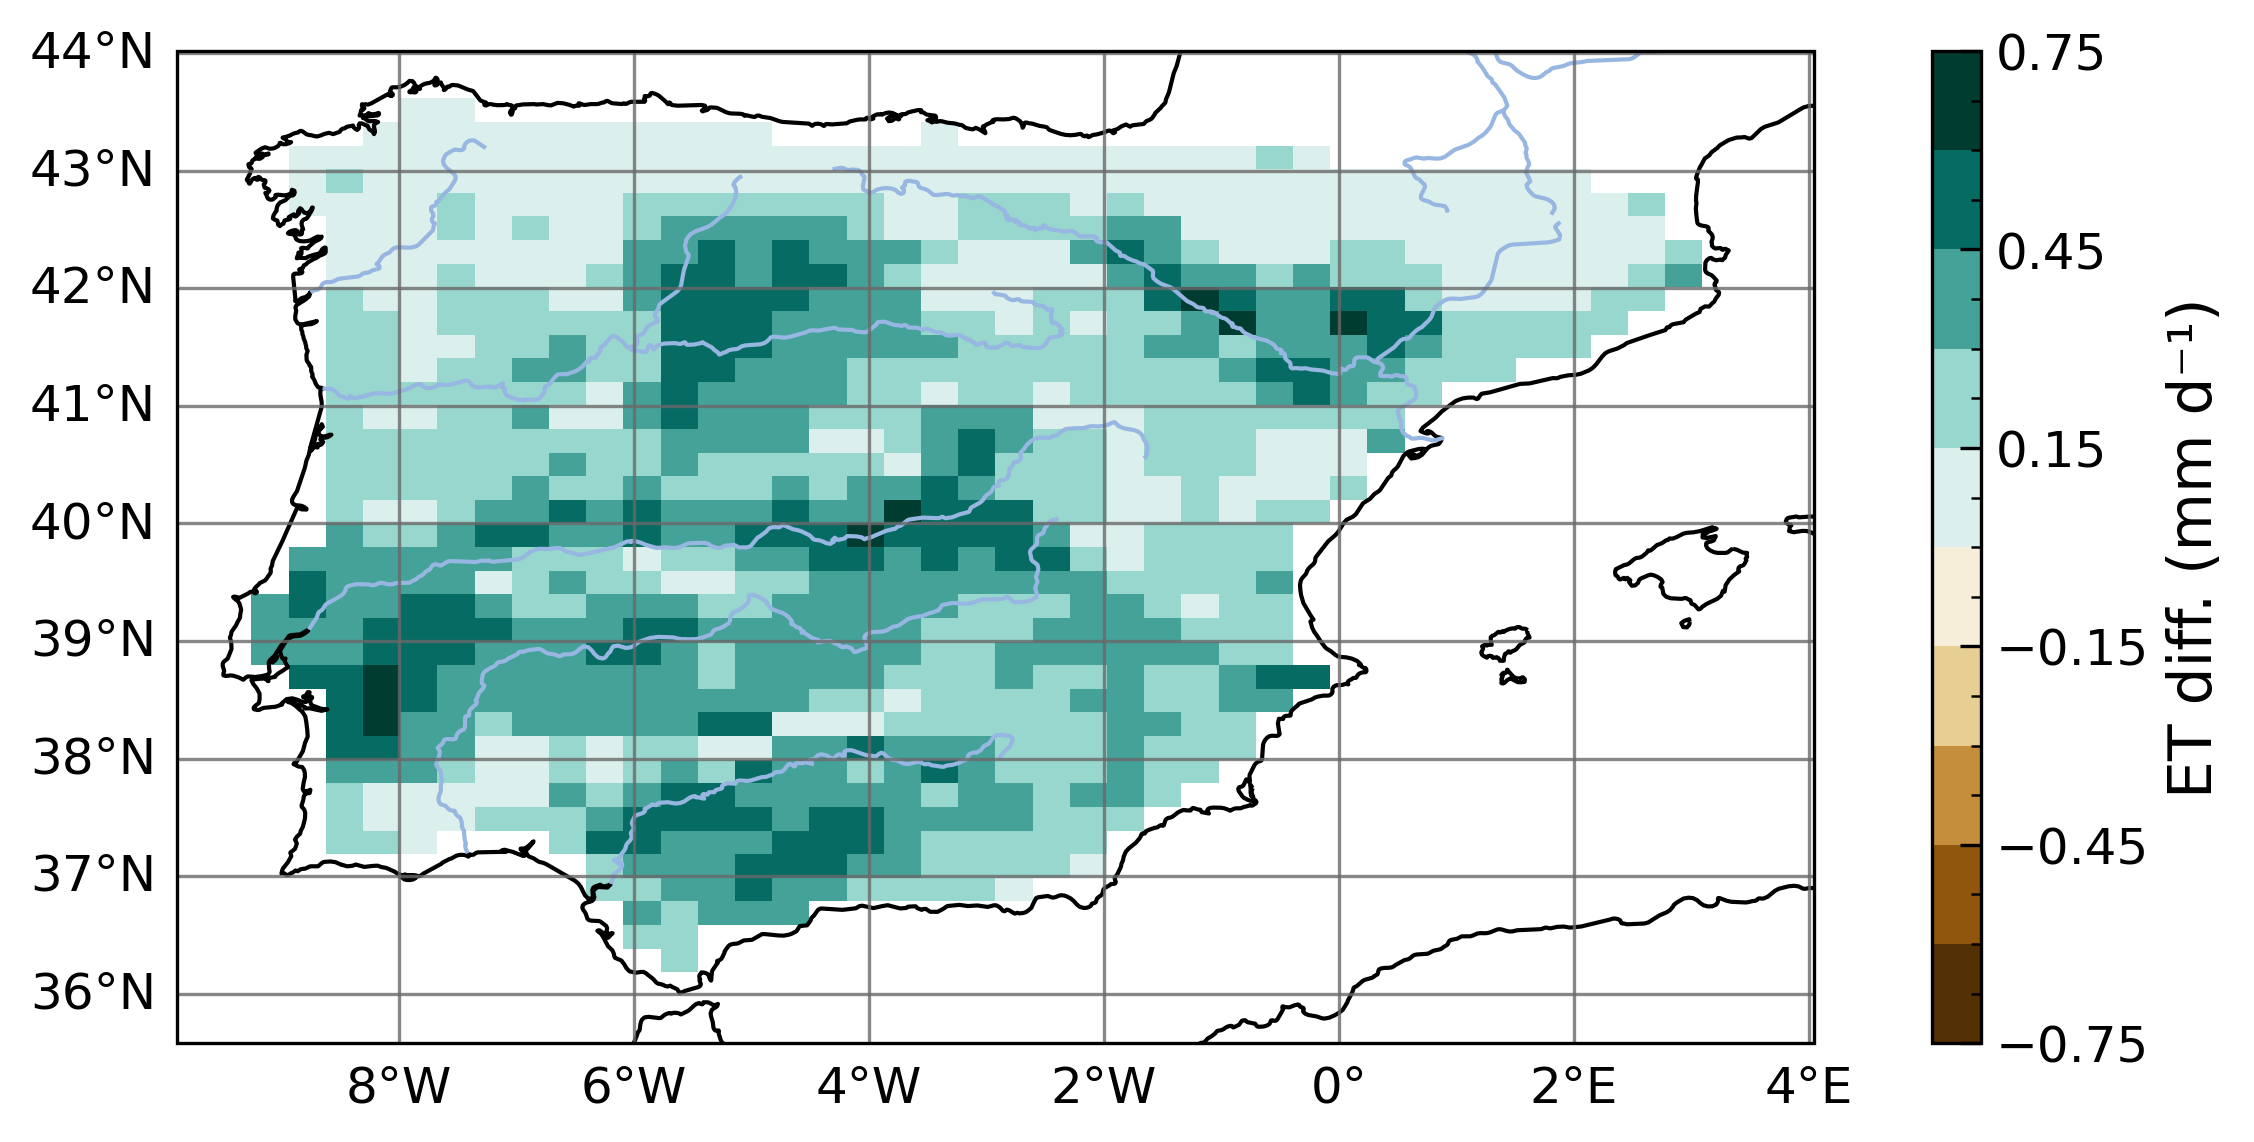
\includegraphics[width=\textwidth]{images/chap4/future/diffmap_evap_futirr.png}
        \end{subfigure} \\

        %q2m
        \begin{subfigure}[b]{0.5\textwidth}
            \caption{2-m specific humidity difference}
            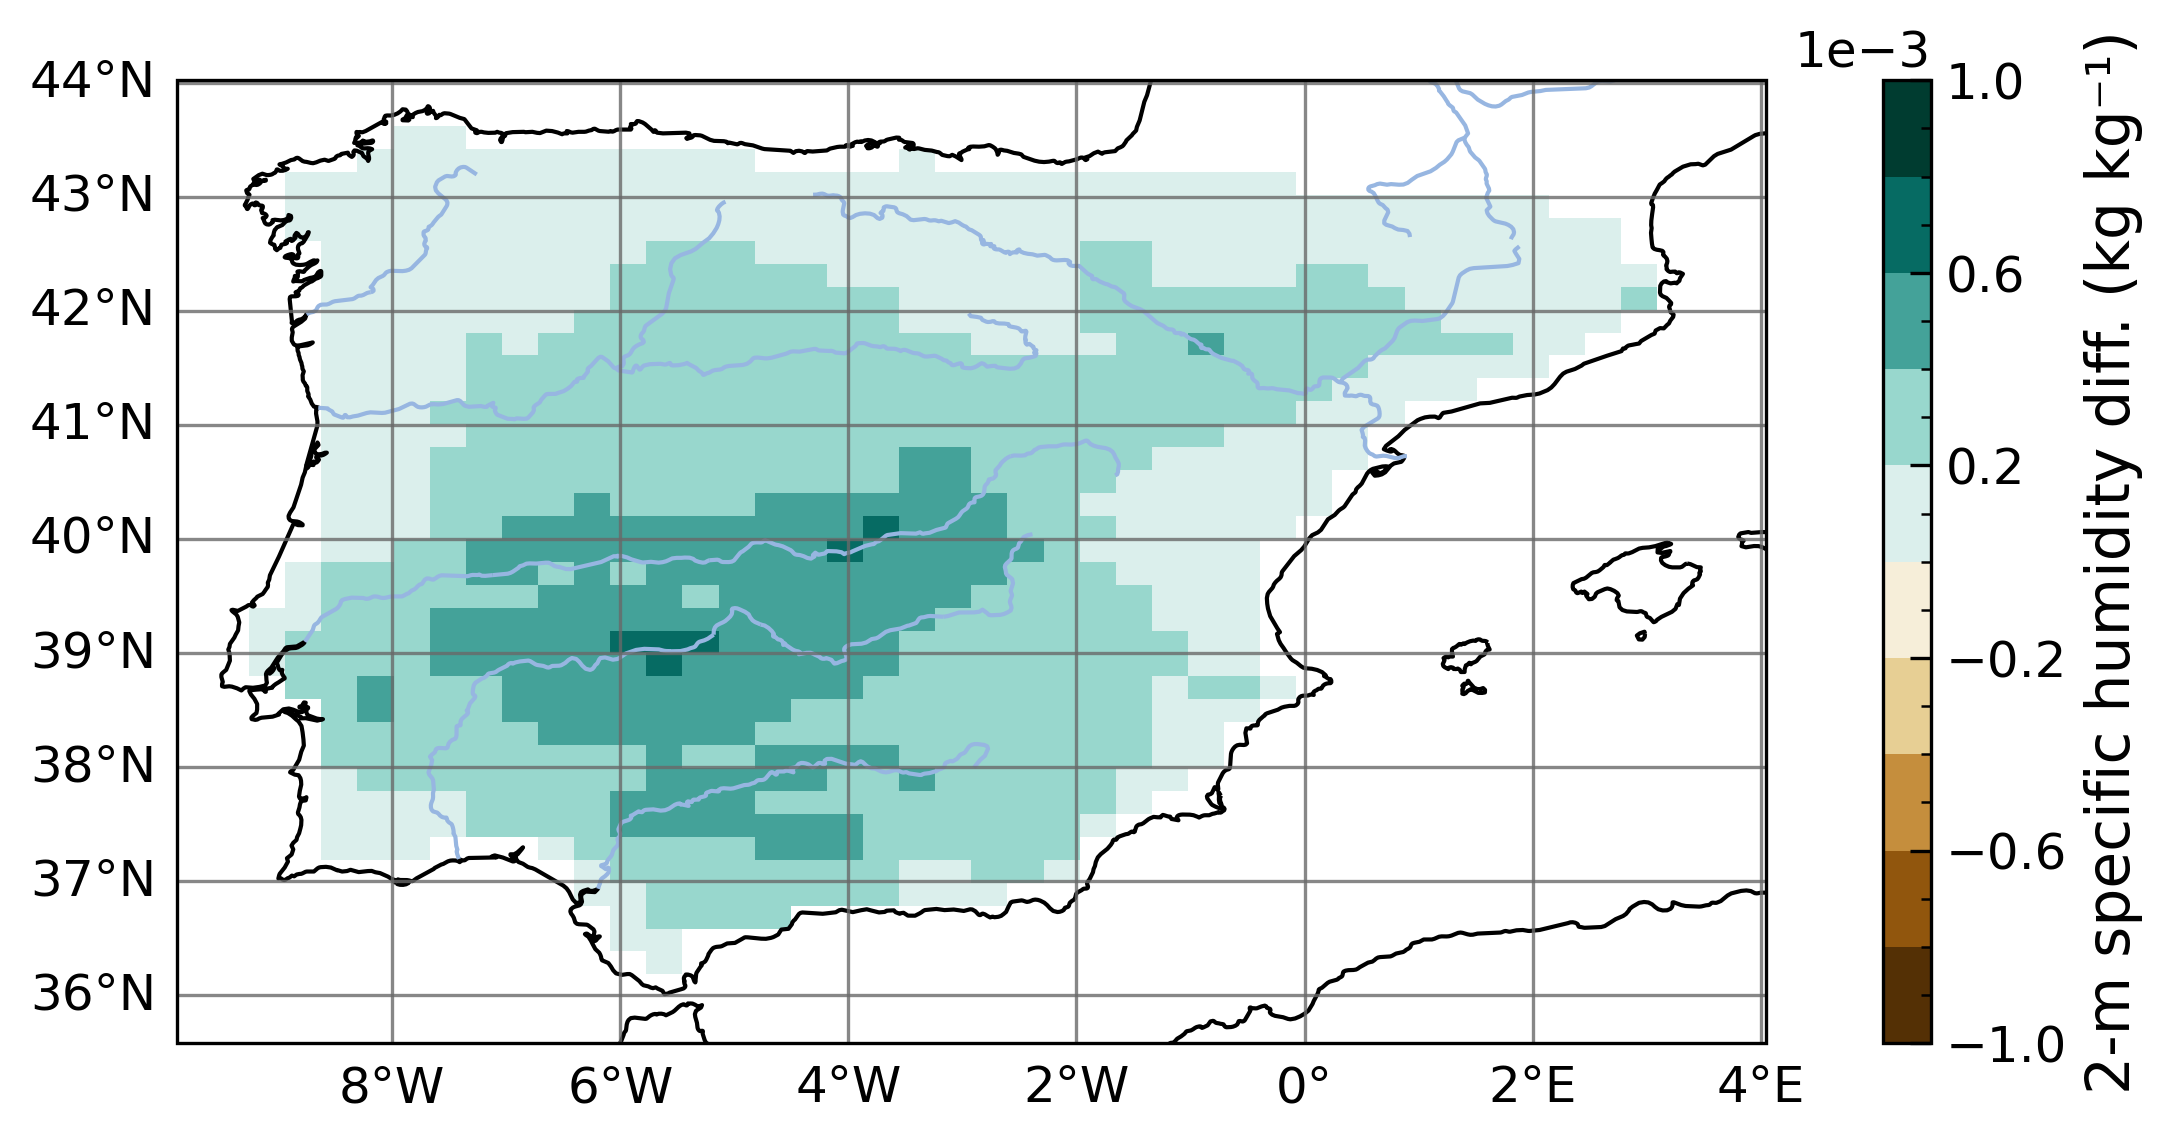
\includegraphics[width=\textwidth]{images/chap4/future/diffmap_q2m_futirr.png}
        \end{subfigure} &
        %rh2m
        \begin{subfigure}[b]{0.5\textwidth}
            \caption{2-m relative humidity difference}
            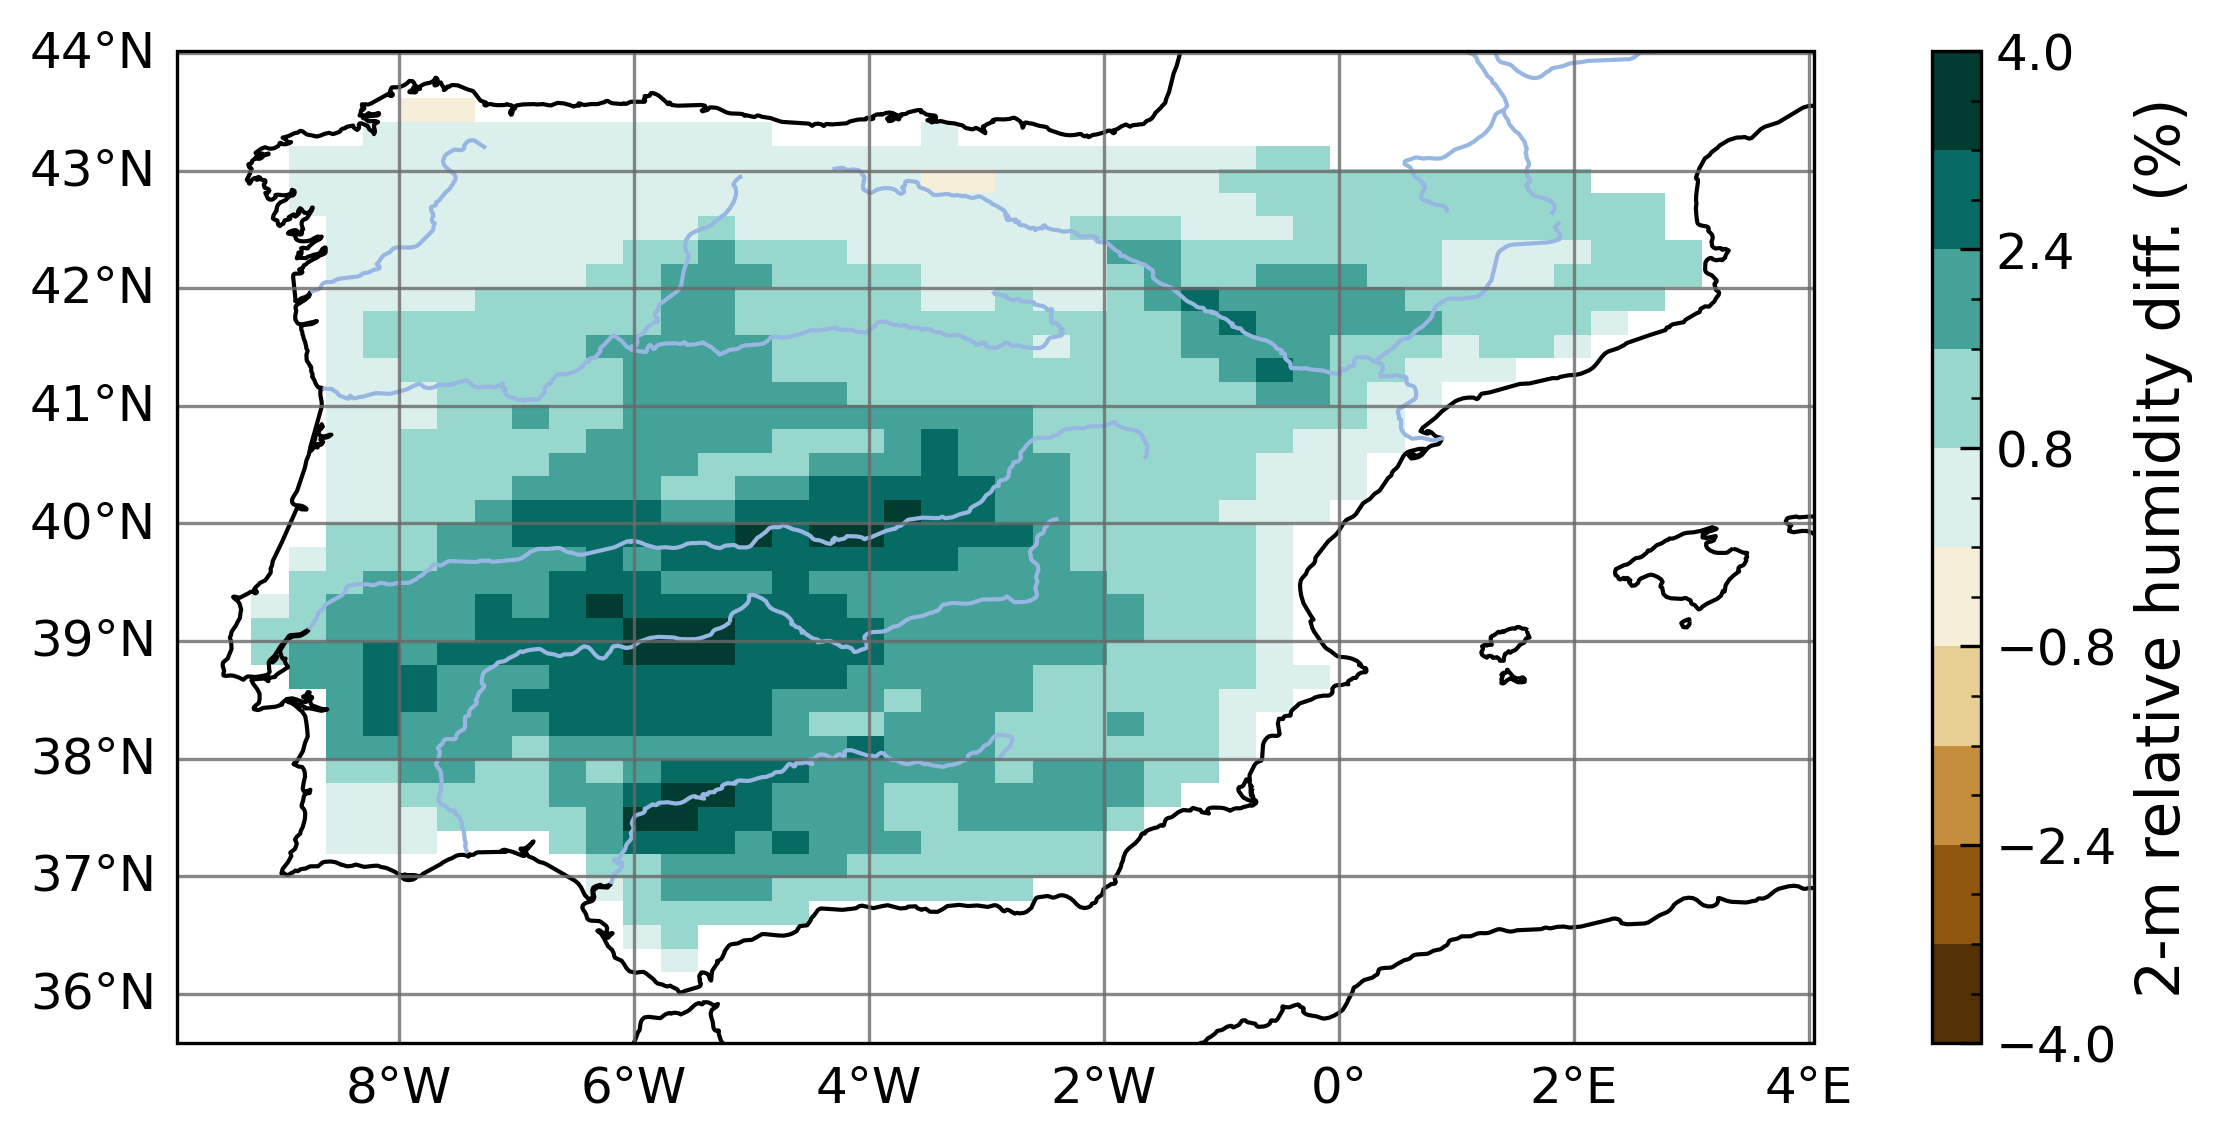
\includegraphics[width=\textwidth]{images/chap4/future/diffmap_rh2m_futirr.png}
        \end{subfigure} \\

        %pblh
        \begin{subfigure}[b]{0.5\textwidth}
            \caption{Atmospheric boundary layer height difference}
            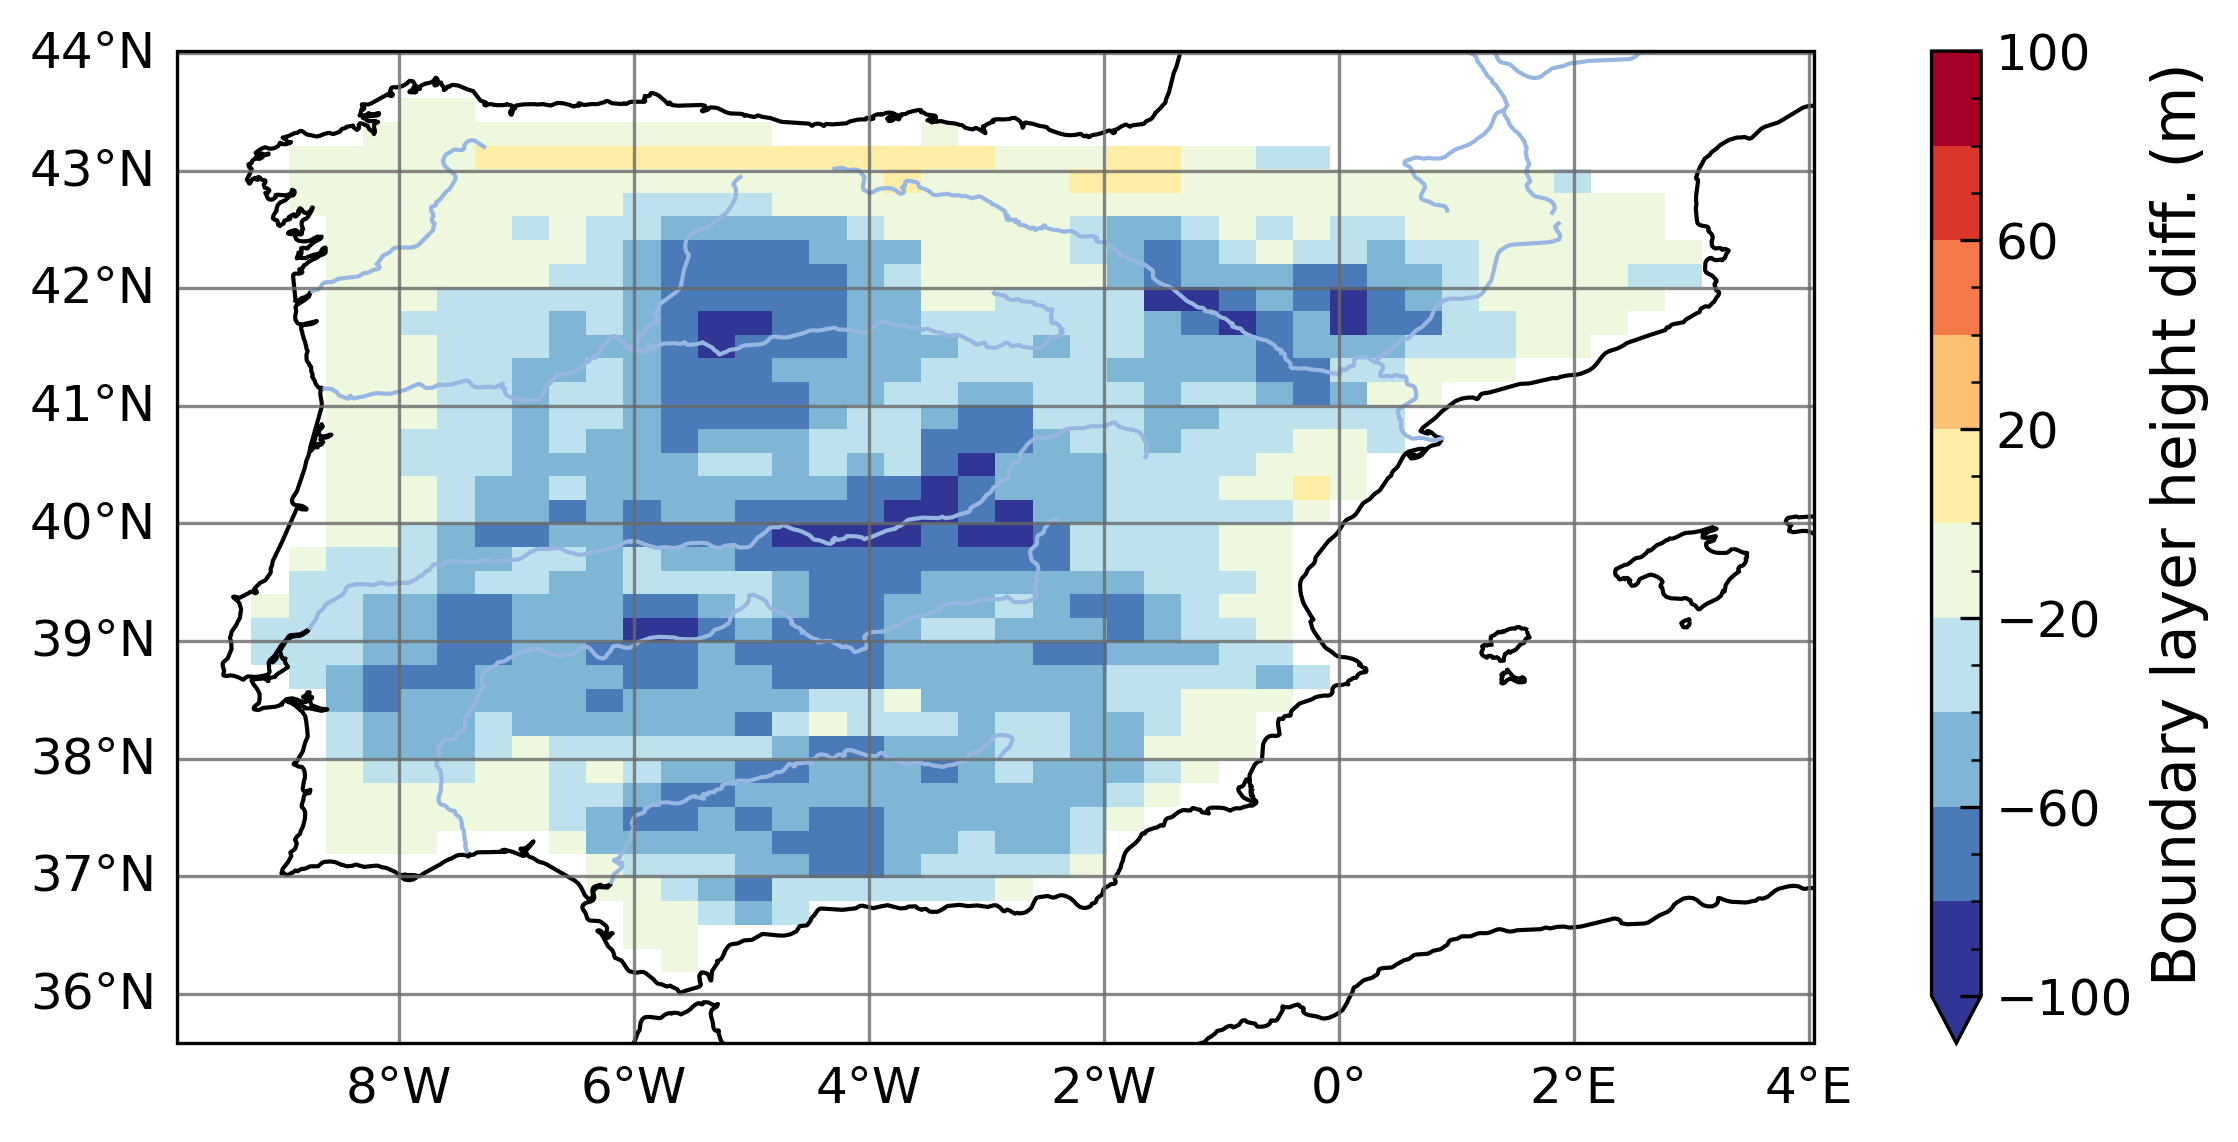
\includegraphics[width=\textwidth]{images/chap4/future/diffmap_s_pblh_futirr.png}
        \end{subfigure} &
        %lcl
        \begin{subfigure}[b]{0.5\textwidth}
            \caption{Lifting condensation level difference}
            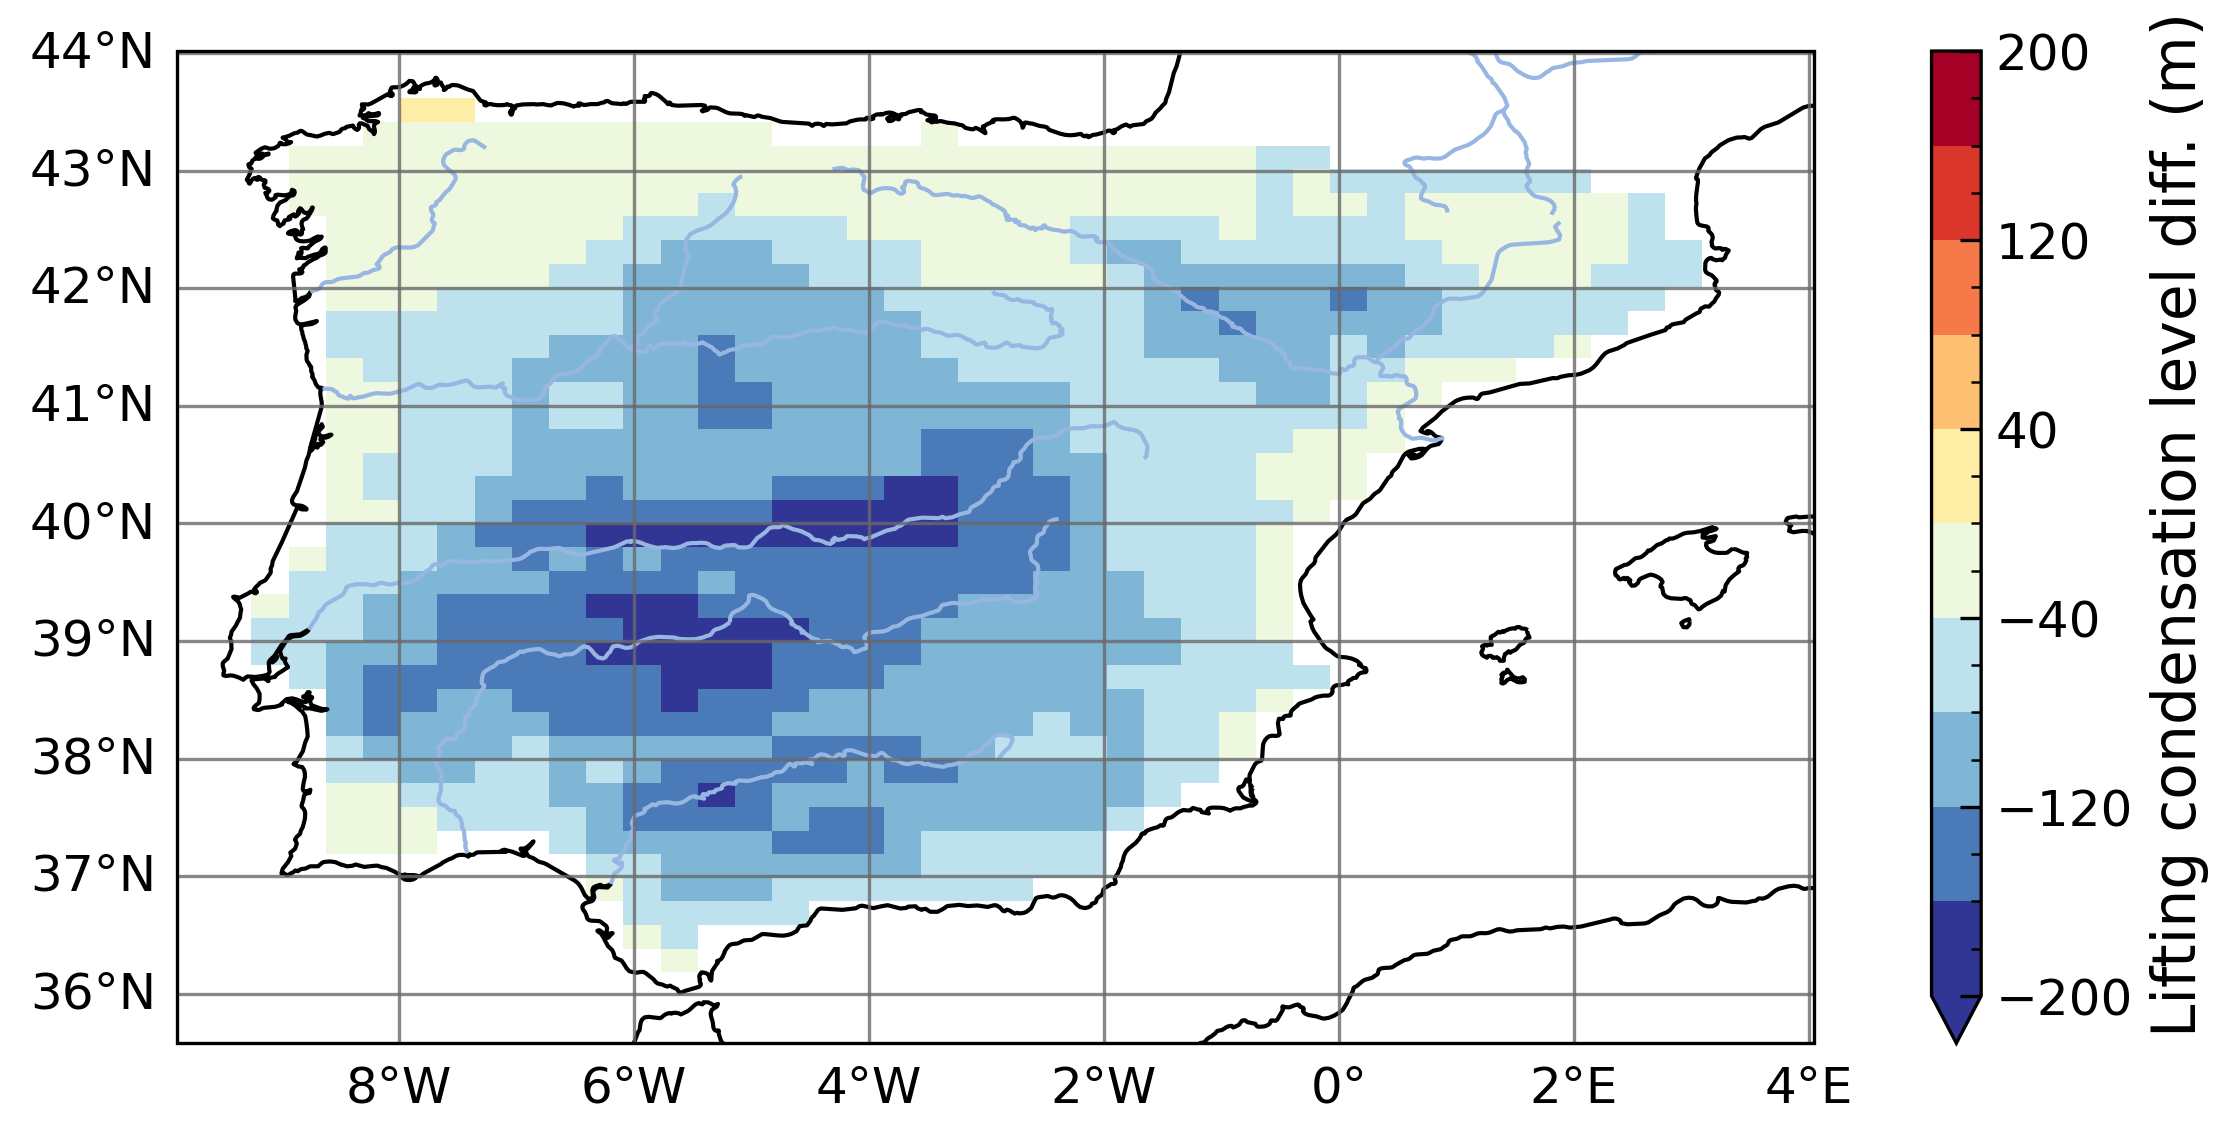
\includegraphics[width=\textwidth]{images/chap4/future/diffmap_s_lcl_futirr.png}
        \end{subfigure} \\
    \end{tabular}
    \caption{Impacts of irrigation under climate change (2050-2062). Annual mean difference between \futirr and \futnoirr.}
    \label{fig:diffmaps_future_irr}
\end{figure}

%IP average if useful 
%precip
% present, no_irr : 2.18771 (mm d⁻¹)
% future, no_irr : 1.86688 (mm d⁻¹)
% future, irr : 1.89212 (mm d⁻¹)
%ET
% present, no_irr : 1.27330 (mm d⁻¹)
% future, no_irr : 1.17734 (mm d⁻¹)
% future, irr : 1.44247 (mm d⁻¹)
%t2m
% present, no_irr : 14.66318 (°C)
% future, no_irr : 16.98357 (°C)
% future, irr : 16.80824 (°C)
%sensible
% present, no_irr : 50.54140 (W m⁻²)
% future, no_irr : 55.53161 (W m⁻²)
% future, irr : 49.91047 (W m⁻²)
%q2m
% present, no_irr : 0.00730 (kg kg⁻¹)
% future, no_irr : 0.00786 (kg kg⁻¹)
% future, irr : 0.00813 (kg kg⁻¹)
%pblh
% present, no_irr : 942.46790 (m)
% future, no_irr : 946.90222 (m)
% future, irr : 909.96997 (m)
%lcl
% present, no_irr : 884.01685 (m)
% future, no_irr : 1039.27222 (m)
% future, irr : 959.86011 (m)
%rh2m
% present, no_irr : 68.83486 (%)
% future, no_irr : 65.23708 (%)
% future, irr : 66.66062 (%)

\clearpage

\subsection{Aridification and impact of irrigation}

Aridity indices are often used as a way to characterize continental regions and how their climate will evolve in the future, under climate change. Aridity aims to describe long-term moisture deficits that limit the development of vegetation. Several definitions and indices have been proposed and used in the last decades, but the most common is the United Nations Environmental Programme (UNEP) aridity index, defined as the ratio of the annual precipitation to potential evapotranspiration : $AI = \frac{P}{PET}$. %todo:refs (Begueria 2025, UNEP 1992)
This index is most relevant when averaged over multiple years to reduce sensitivity to specific droughts or extreme precipitation events.

At the end of Mariame Maiga's internship, a short study of the evolution of aridity under climate change was conducted, using this index to classify grid cells into five aridity classes as presented in Table \ref{table:aridity_classes}. 
Potential evapotranspiration was computed the Penman-Monteith equation, matching the formulation used with observation data over the Iberian Peninsula in \citet{begueria_aridity_2025}.
%taken from ORCHIDEE's \textit{evapot\_corr} variable, which is computed by applying a correction from \citet{milly_potential_1992} to the formulation given for $E_{pot}$ in Chapter \ref{chap:methods}.

\begin{table}[h]
    \centering
    \begin{tabular}{|l|l|}
        \hline
        \textbf{Aridity class} & \textbf{Index values} \\
        \hline
        Hyper-arid & \( AI < 0.05 \) \\
        \hline
        Arid & \( 0.05 < AI < 0.2 \) \\
        \hline
        Semi-arid & \( 0.2 < AI < 0.5 \) \\
        \hline
        Dry sub-humid & \( 0.5 < AI < 0.65 \) \\
        \hline
        Humid & \( 0.65 < AI \) \\
        \hline
    \end{tabular}
    \caption{Aridity classes based on UNEP aridity index values.}
    \label{table:aridity_classes}
\end{table}

The spatial distribution in the \presnoirr simulation (Fig. \ref{fig:aridity_index_v2}a, b) shows a dominant semi-arid climate over the Iberian Peninsula, with a humid strip in the northern coast and the Pyrenees, and arid climate in the Ebro and Guadalquivir valleys, and other areas in the South.
Index values are much more arid than the results obtained from observations for the period 1991-2020 in \citet{begueria_aridity_2025}, which did not show any arid area and a larger extent of the dry sub-humid areas. This might be explained by the more recent period considered since the effects of climate change are already observed in the Iberian Peninsula.
Furthermore, the way to compute the 2-meter variables used to obtain PET and the more generic biases of the model can have a strong impact on the value of the aridity index and on the classification of each grid cell. However, this simple index remains an interesting tool to study the future evolution of aridity in the various regions of the Peninsula by comparing simulations to one another.
Under the SSP5-8.5 climate change scenario, in \futnoirr (Fig. \ref{fig:aridity_index_v2}c, d), the share of humid grid cells falls from 19.4\% to 11.0\%, the share of semi-arid and dry sub-humid cells is reduced by respectively 1 and 2 percentage points, while the share or arid grid cells is more than doubled, from 8.0\% to 19.9\%. This corresponds to a shift in each aridity class. Most humid areas change to dry sub-humid or even directly to semi-arid, leaving only the heart of the Pyrenees and of the north-western mountain ranges in this aridity class. The arid areas, on the contrary, extend to encompass a large share of the Ebro, Guadiana and Guadalquivir valleys. This shift in aridity is consistent with the changes described in Fig. \ref{fig:diffmaps_present_future}, a decrease of precipitation and an increase in temperature (which partly drives PET).

The influence of irrigation on this evolution under climate change remains limited (Fig. \ref{fig:aridity_index_v2}). The share of arid grid cells is lower in \futirr (16.2\%) than \futnoirr (19.9\%), which is mostly compensated by a larger share of semi-arid grid cells (65.3\% instead of 62.9\%) whereas the share of humid cells increase by one percentage point. Irrigation has an effect on the aridity index through the moistening and cooling of the lower atmosphere, which can decrease PET, and through the changes in precipitation. As described in Fig. \ref{fig:diffmaps_future_irr}, the cooling induced by irrigation is rather small compared to the warming induced by climate change, and the increases in precipitation are mostly located in the elevated areas. This explains why irrigation is not able to limit the expansion of the arid areas in the valleys under climate change.
The results presented here are clearly dependent on the the choice of the aridity index and on the biases of the model for near-surface variables and precipitation, which would require further investigation. In practical terms, they still suggest that although irrigation is an adaptation strategy which can help sustaining plant growth in the valleys, it has very limited long-term benefits on the local and regional climate over cultivated areas.

%figure : maps of aridity index classes for present and future
\begin{figure}[htbp]
    \centering
    %pres, no_irr
    \begin{subfigure}[b]{0.42\textwidth}
        \caption{Aridity index classes in \presnoirr}
        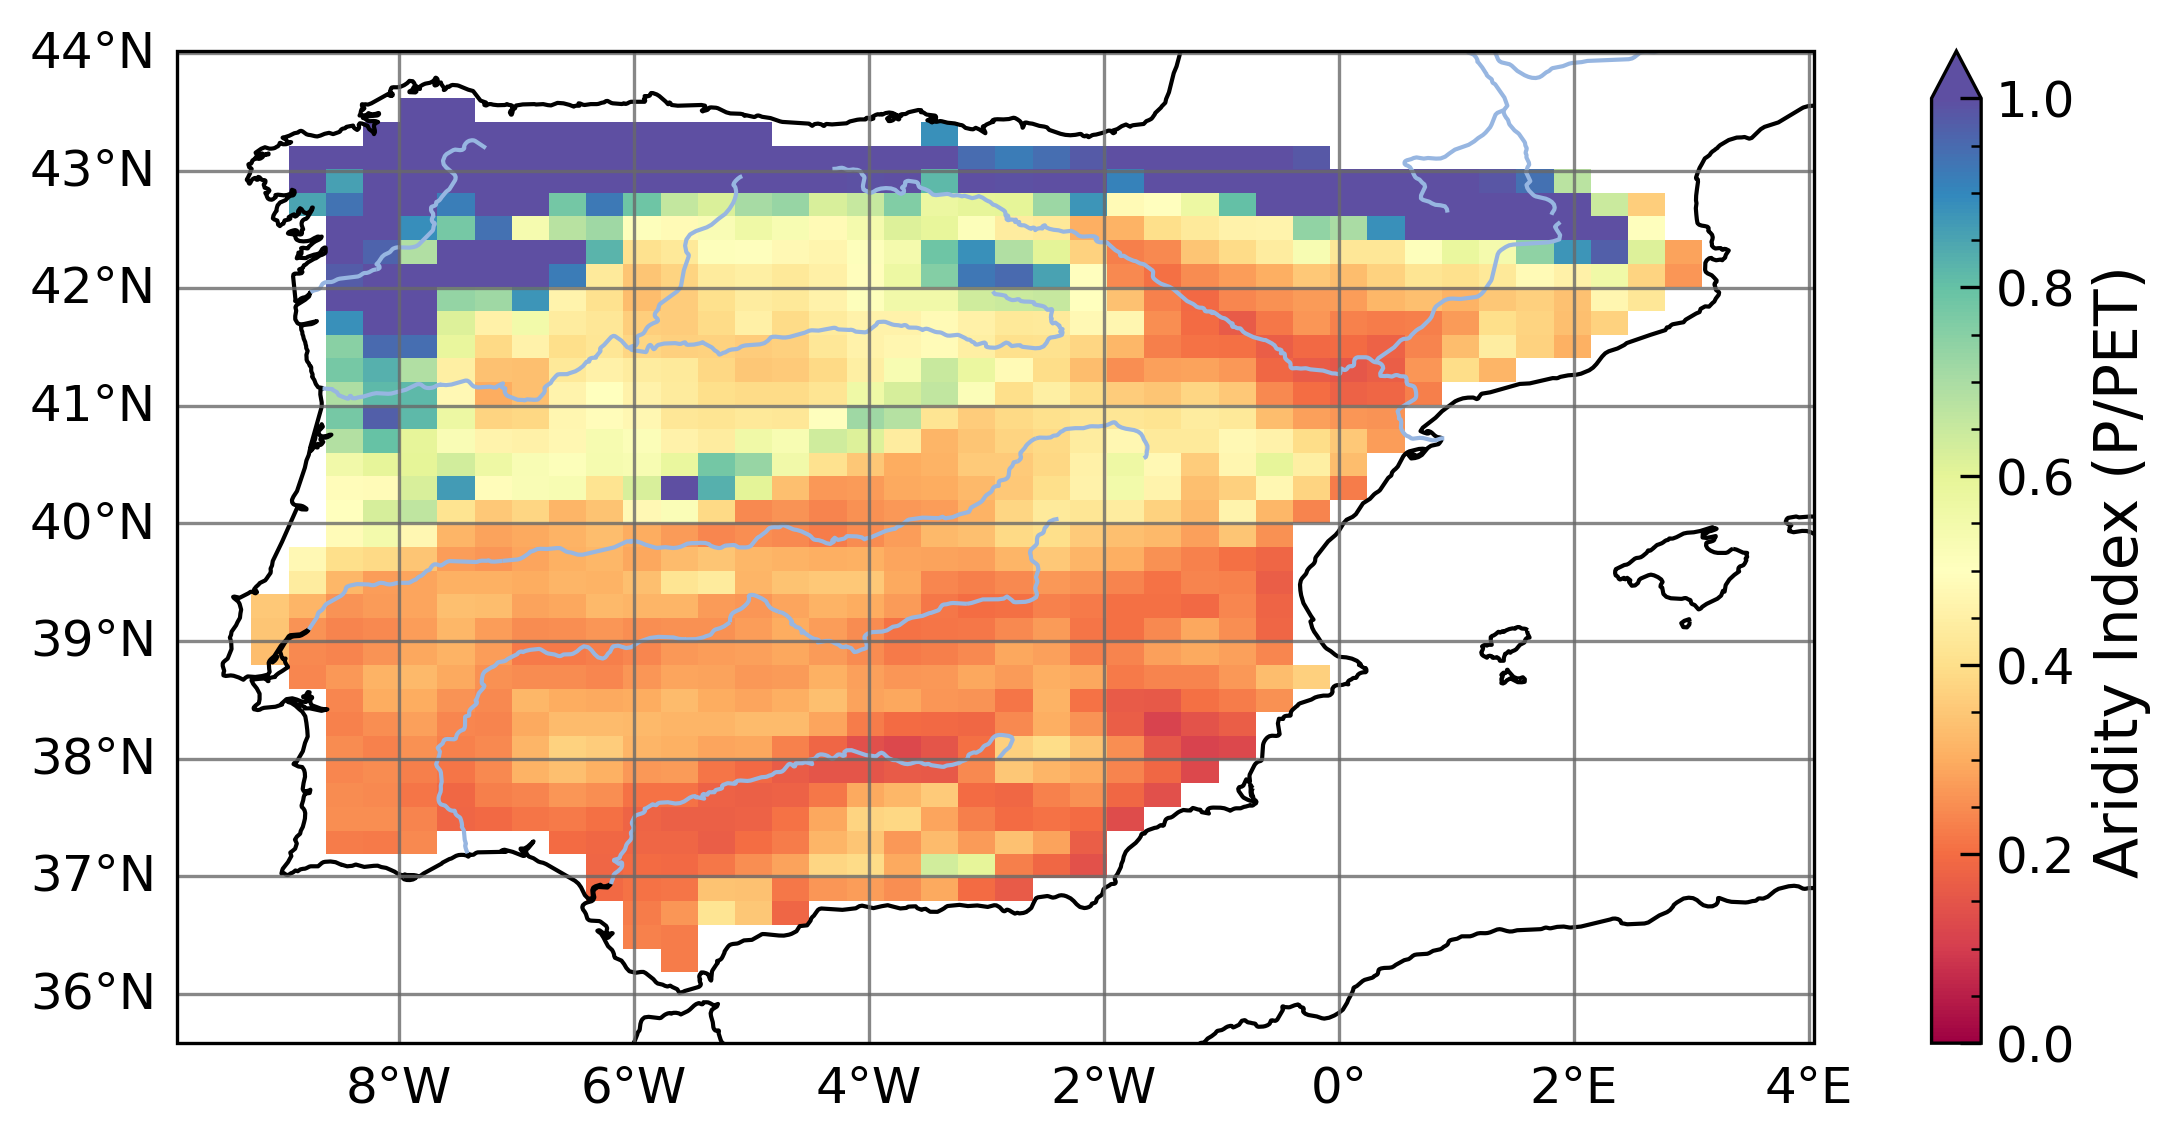
\includegraphics[width=\textwidth]{images/chap4/future/map_AI_pres_noirr.png}
    \end{subfigure}
    \begin{subfigure}[b]{0.48\textwidth}
        \caption{Aridity index classes in \presnoirr}
        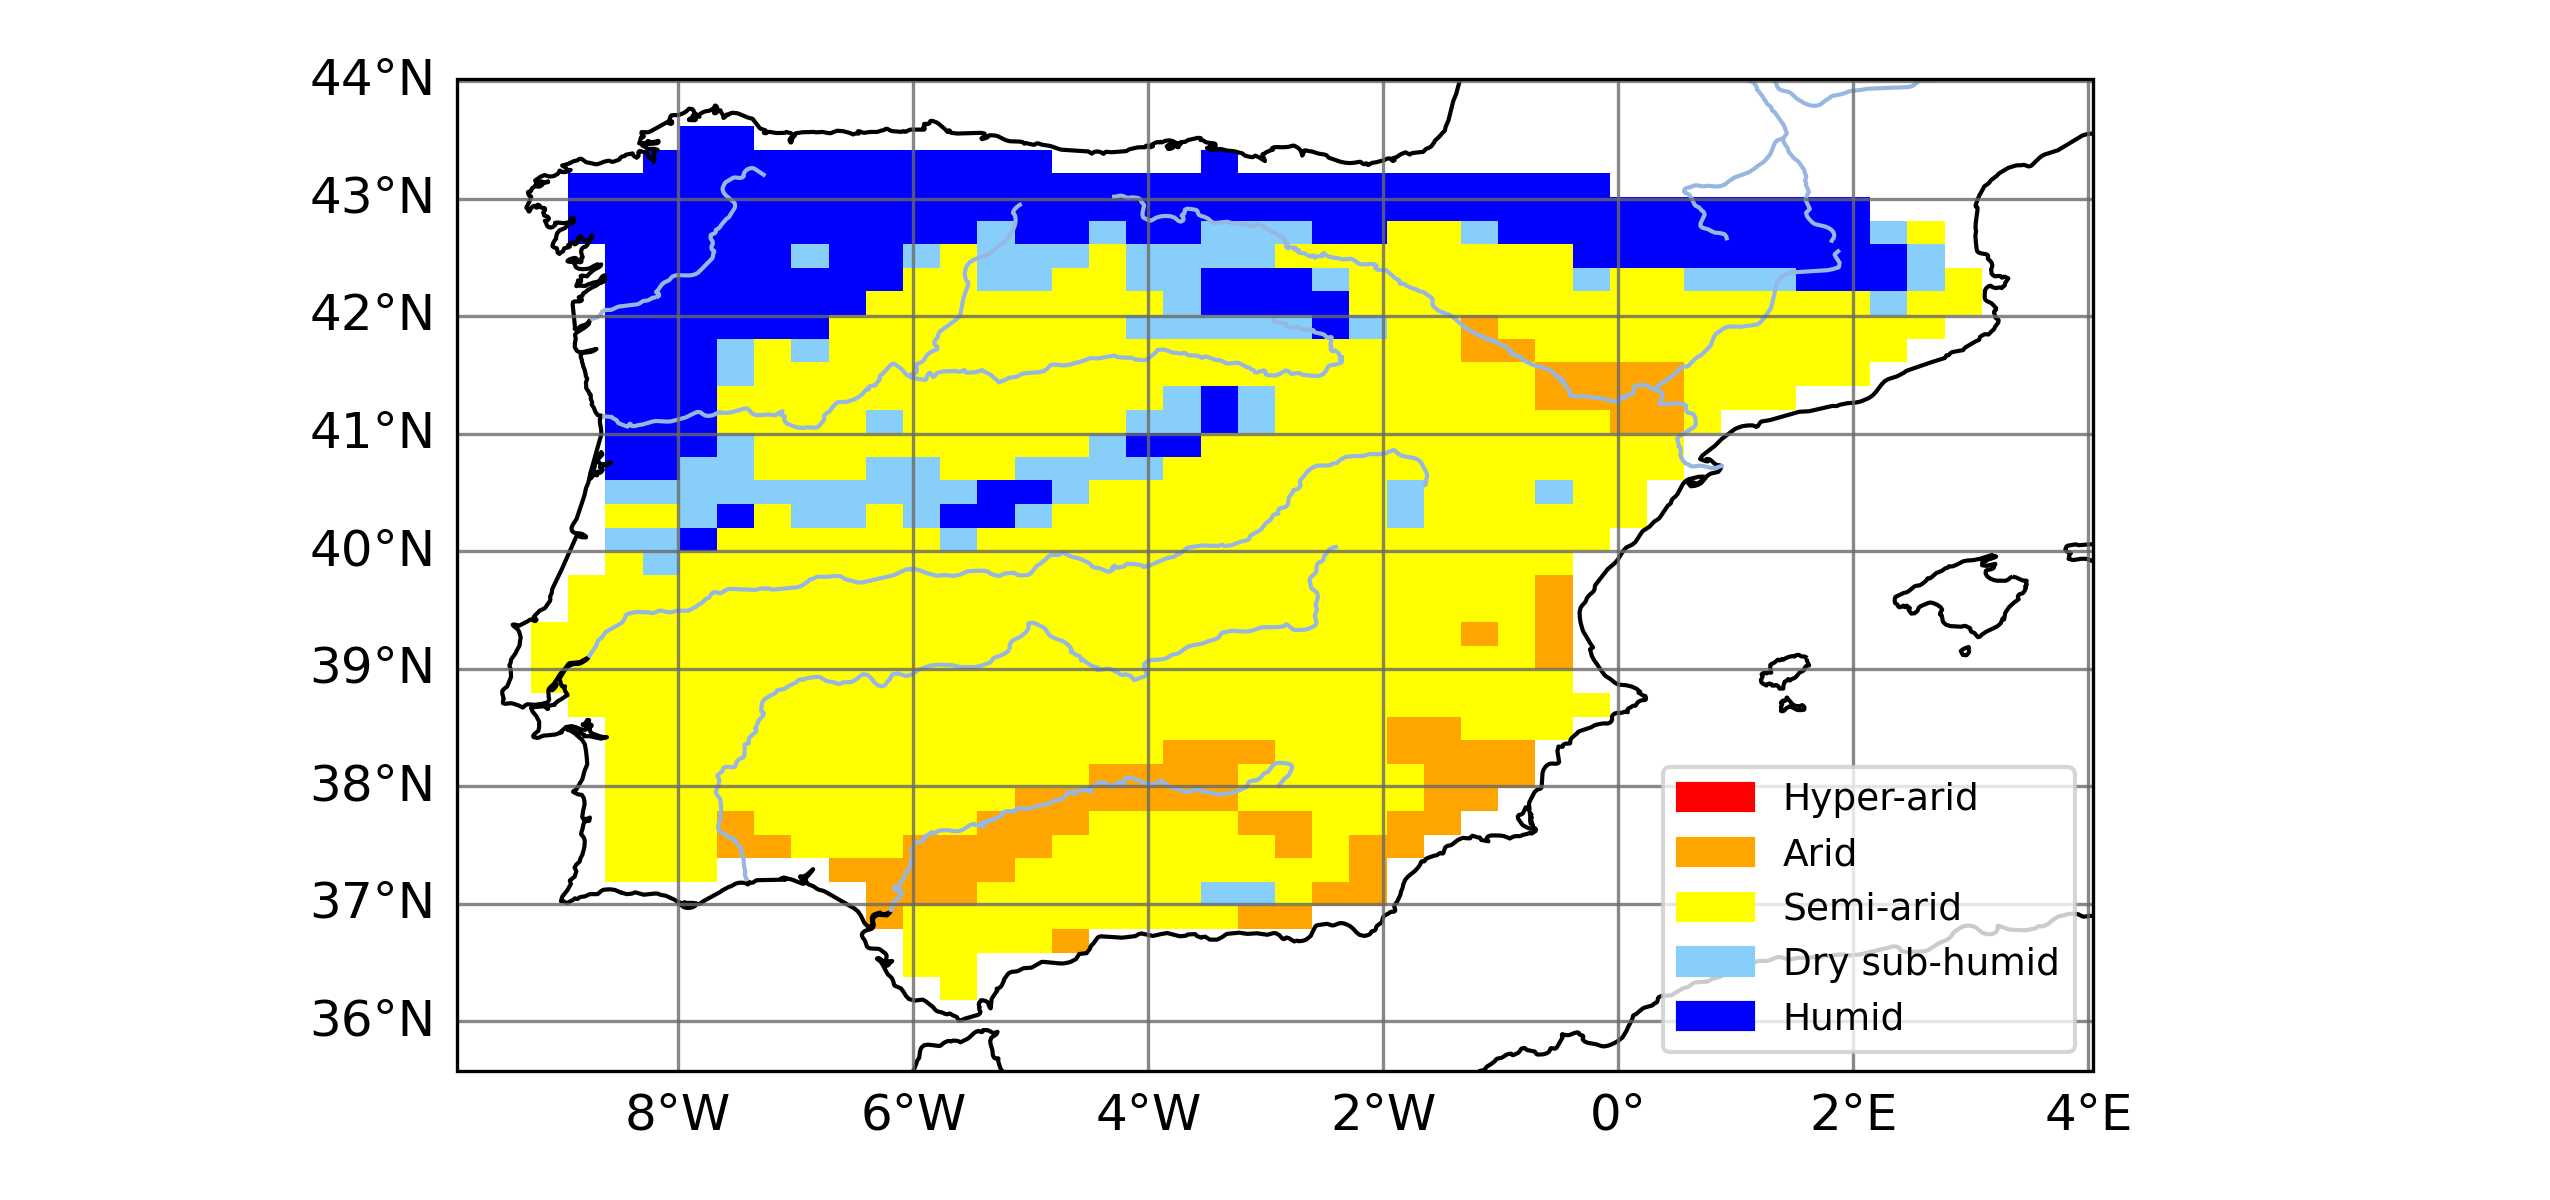
\includegraphics[width=\textwidth]{images/chap4/future/aridity_index_pres_noirr.png}
    \end{subfigure} \\

    %future, noirr
    \begin{subfigure}[b]{0.42\textwidth}
        \caption{Aridity index in \futnoirr}
        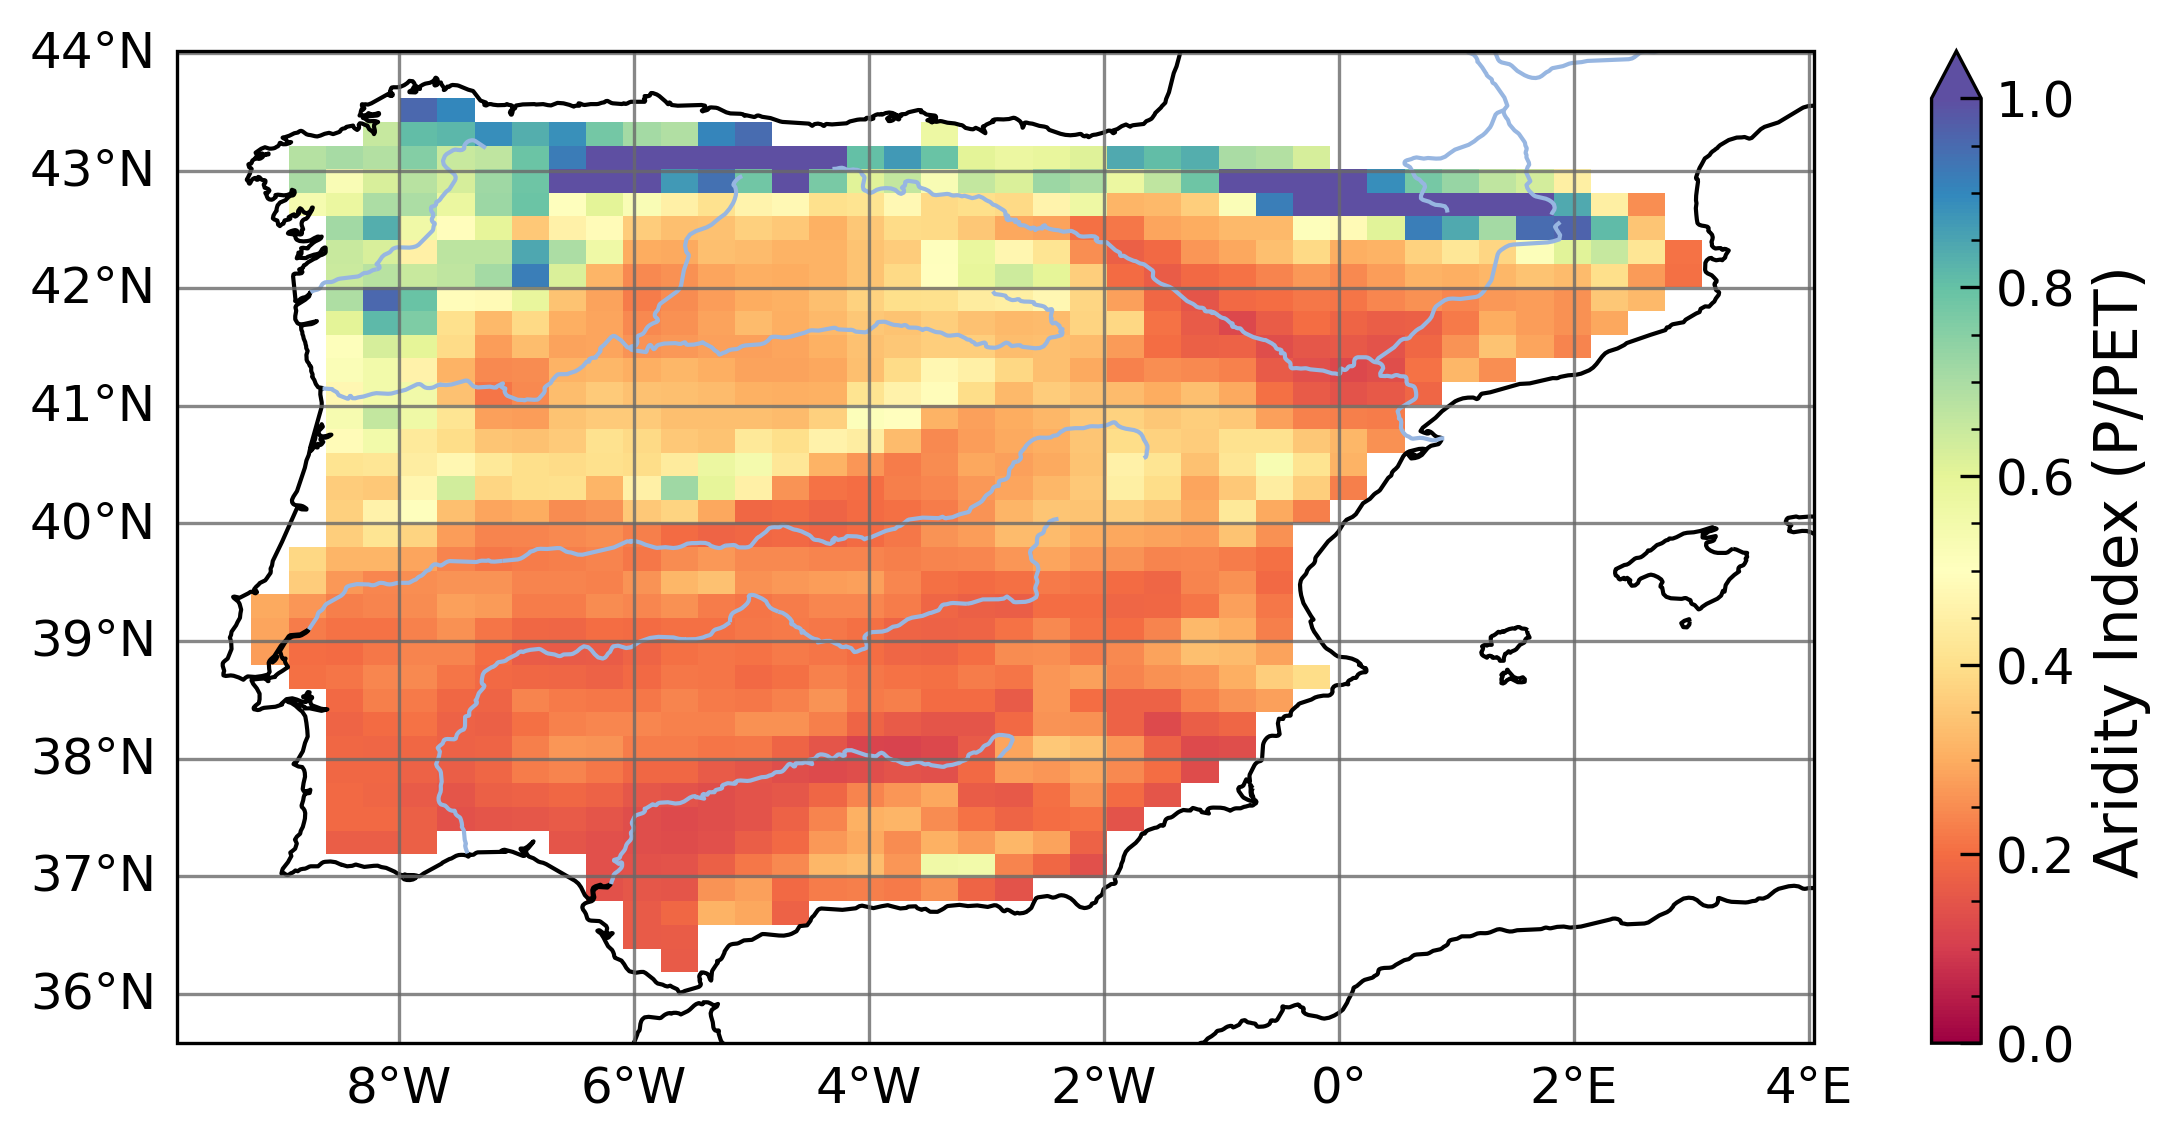
\includegraphics[width=\textwidth]{images/chap4/future/map_AI_fut_noirr.png}
    \end{subfigure}
    \begin{subfigure}[b]{0.48\textwidth}
        \caption{Aridity index classes in \futnoirr}
        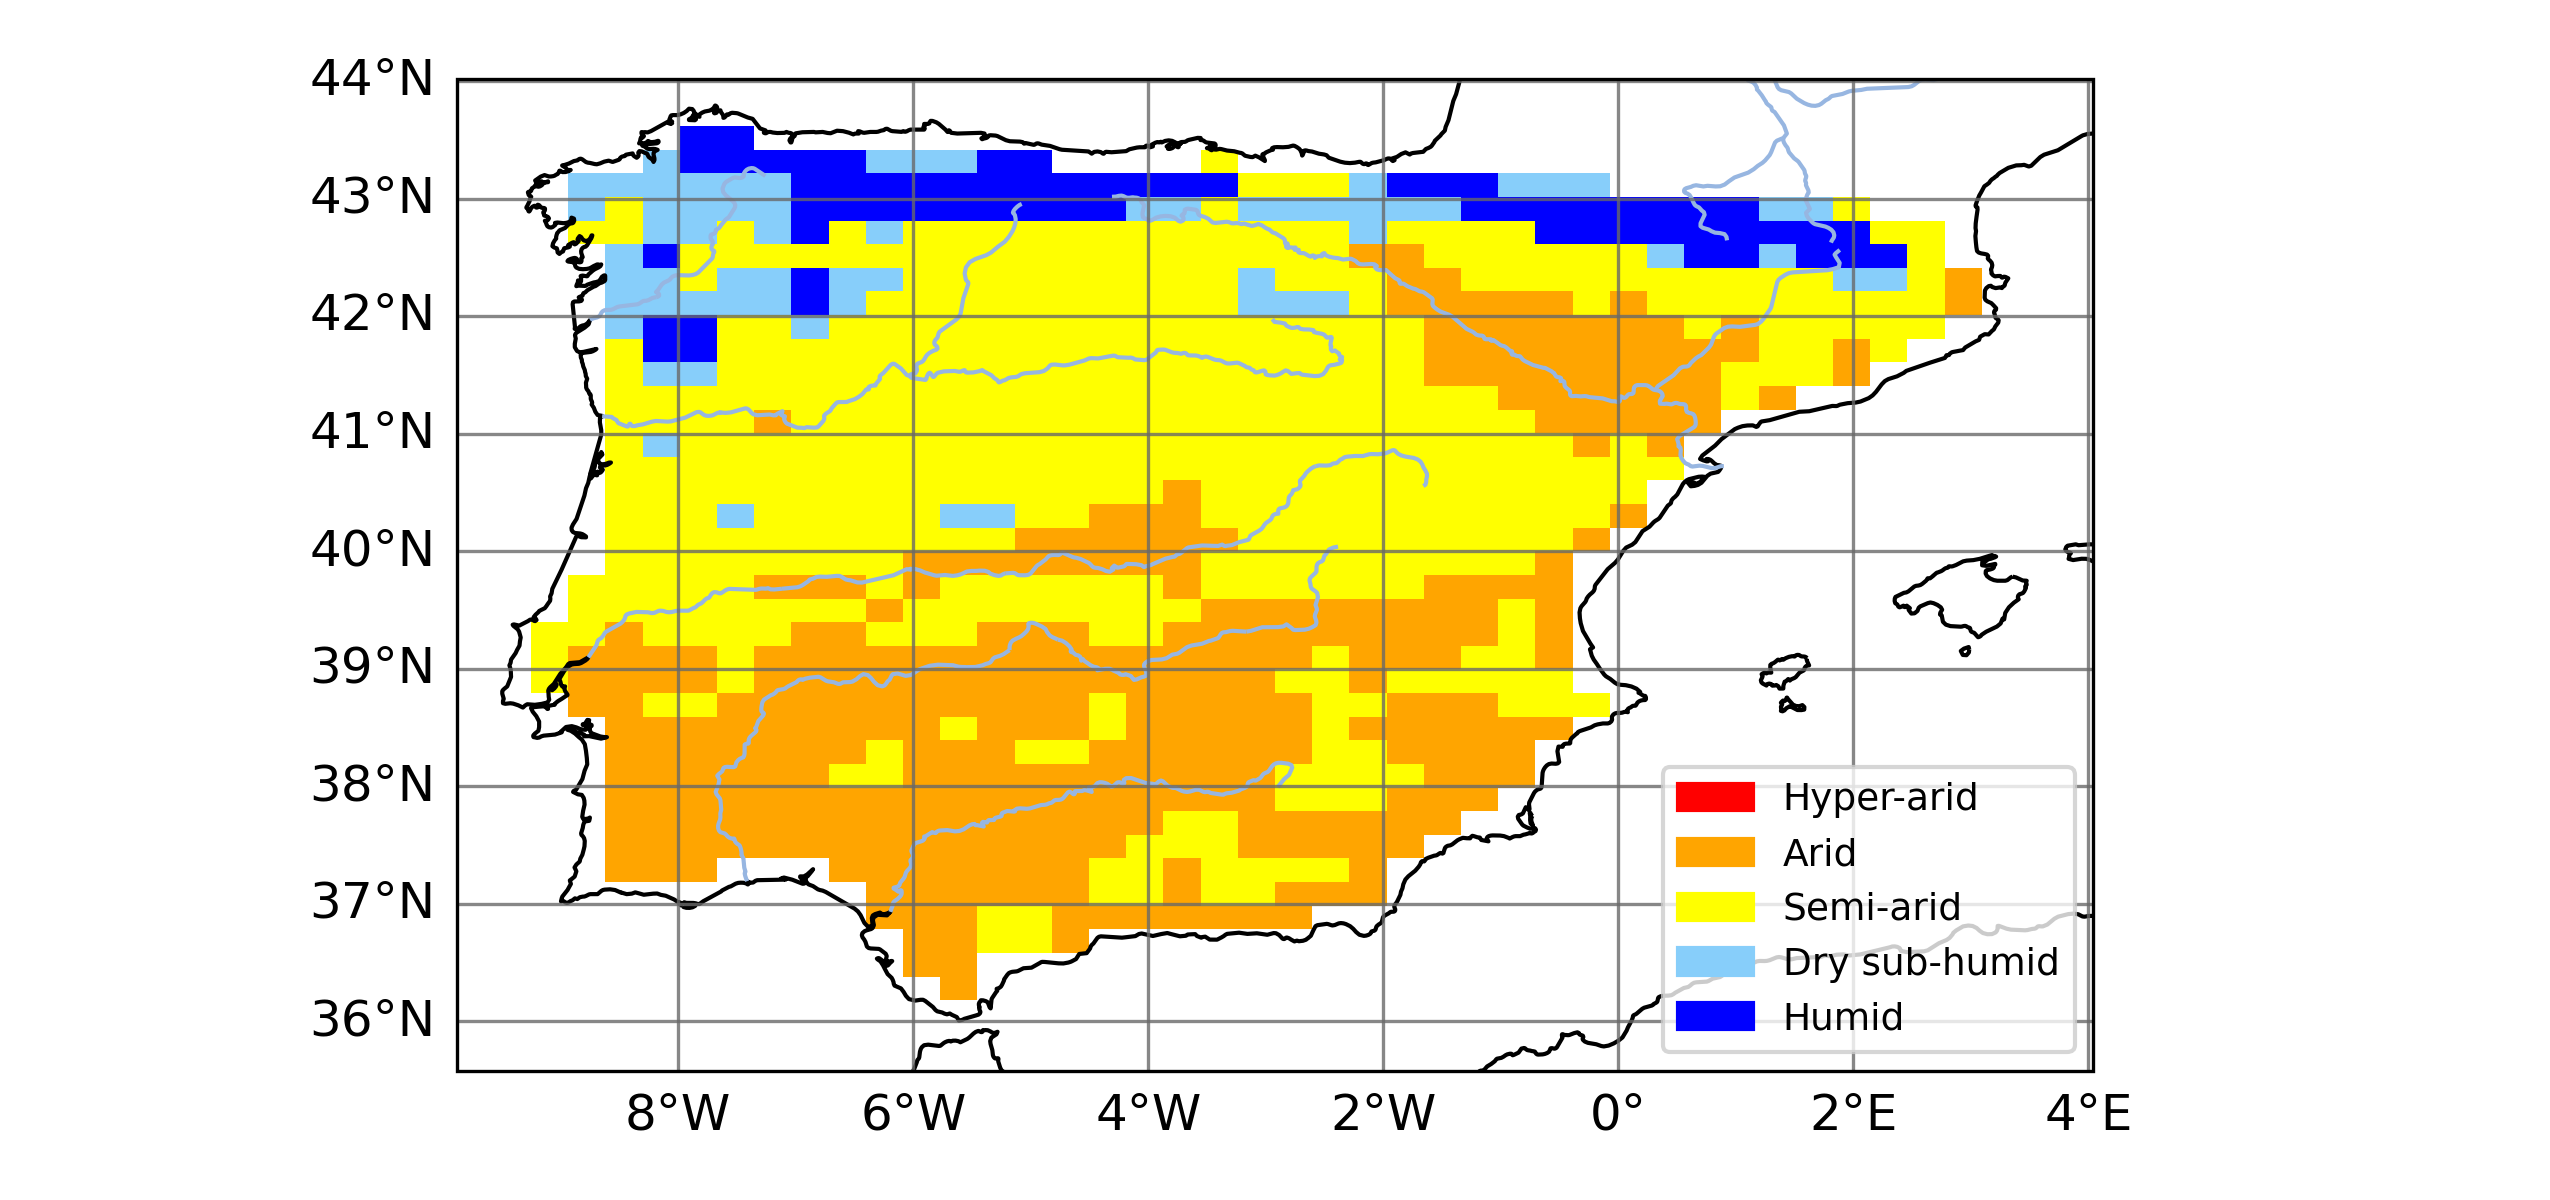
\includegraphics[width=\textwidth]{images/chap4/future/aridity_index_fut_noirr.png}
    \end{subfigure} \\

    %future, irr
    \begin{subfigure}[b]{0.42\textwidth}
        \caption{Aridity index in \futirr}
        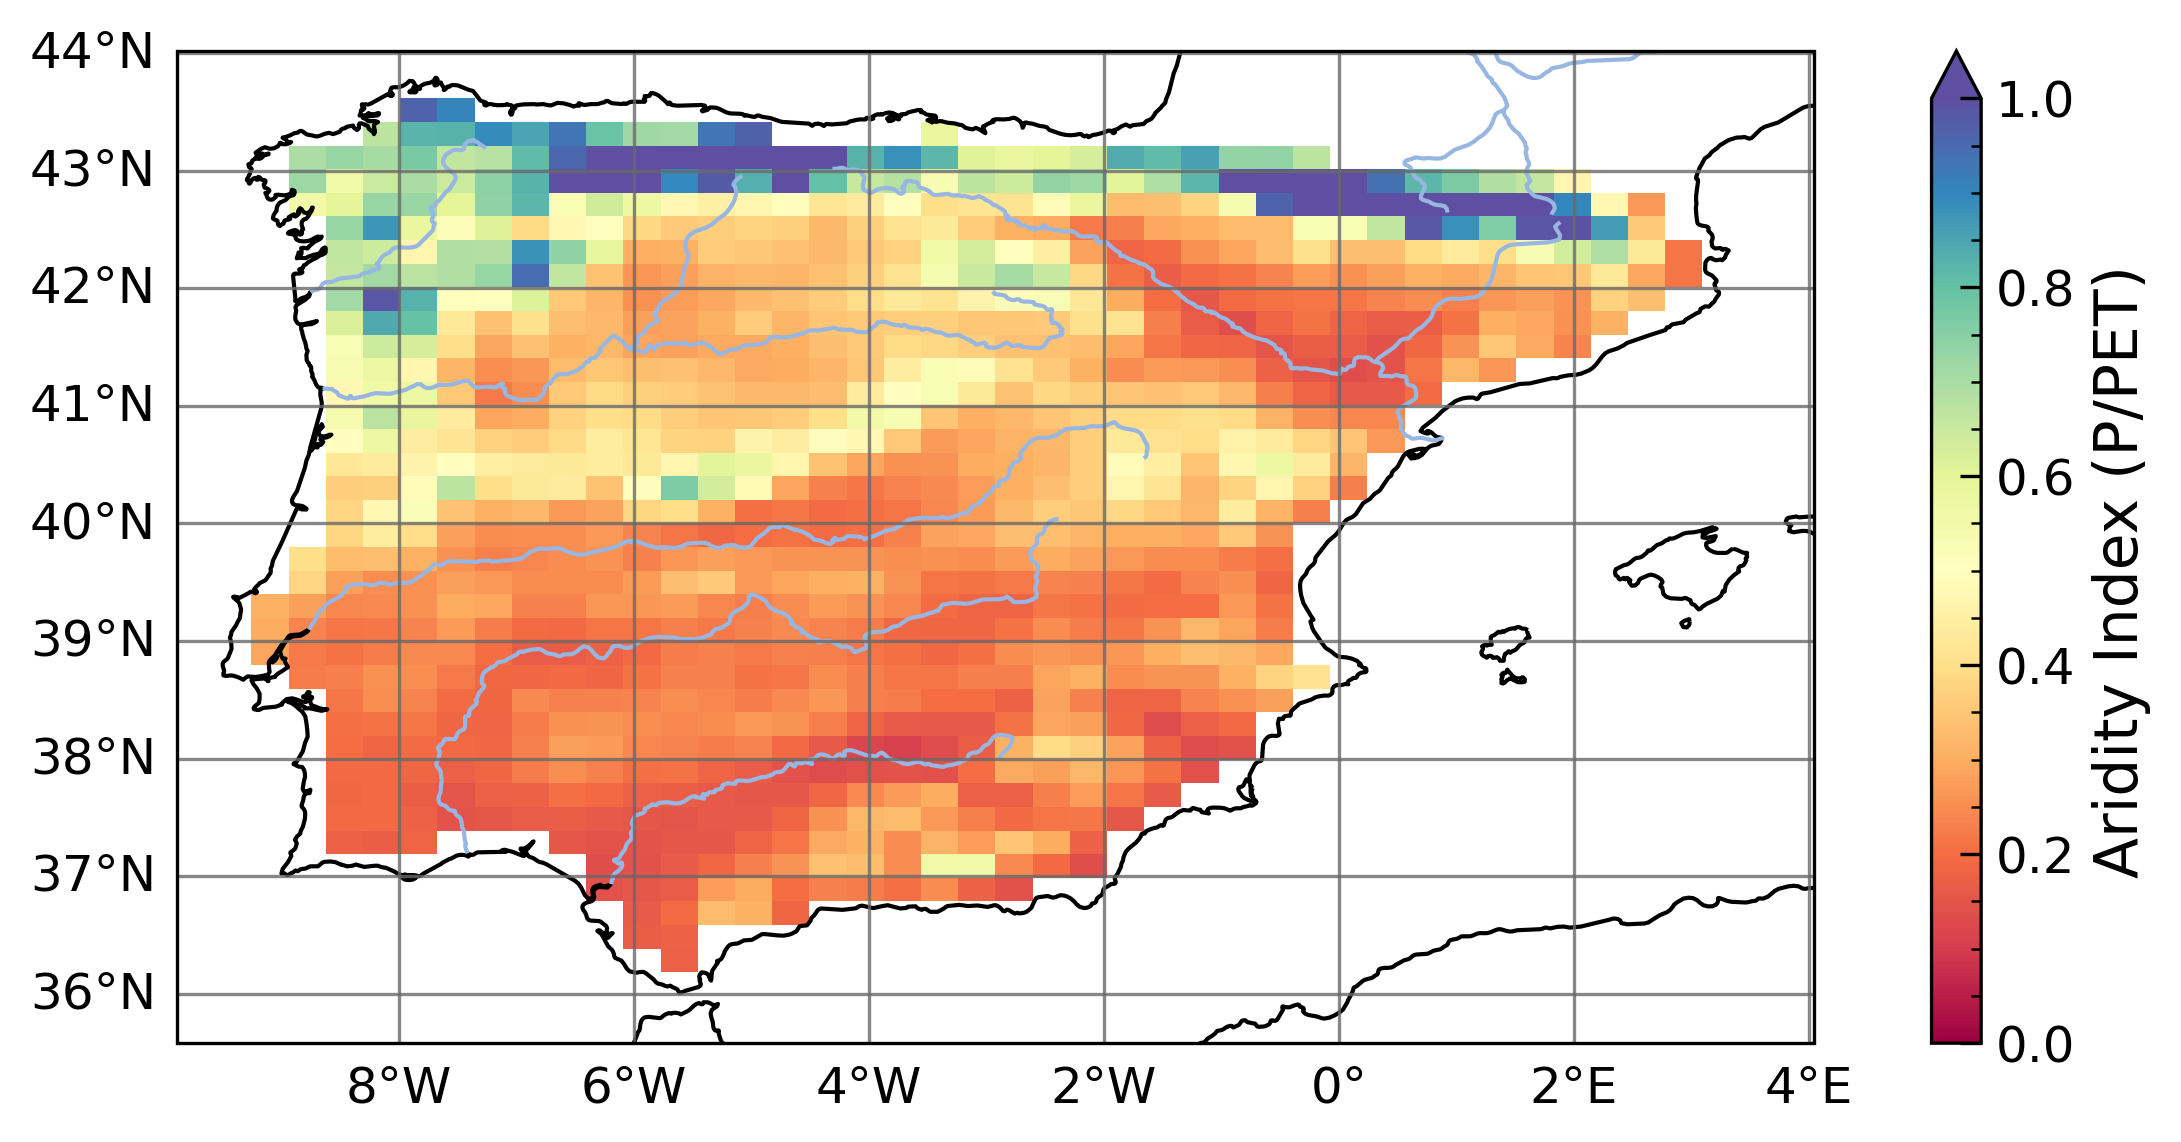
\includegraphics[width=\textwidth]{images/chap4/future/map_AI_fut_irr.png}
    \end{subfigure}
    \begin{subfigure}[b]{0.48\textwidth}
        \caption{Aridity index classes in \futirr}
        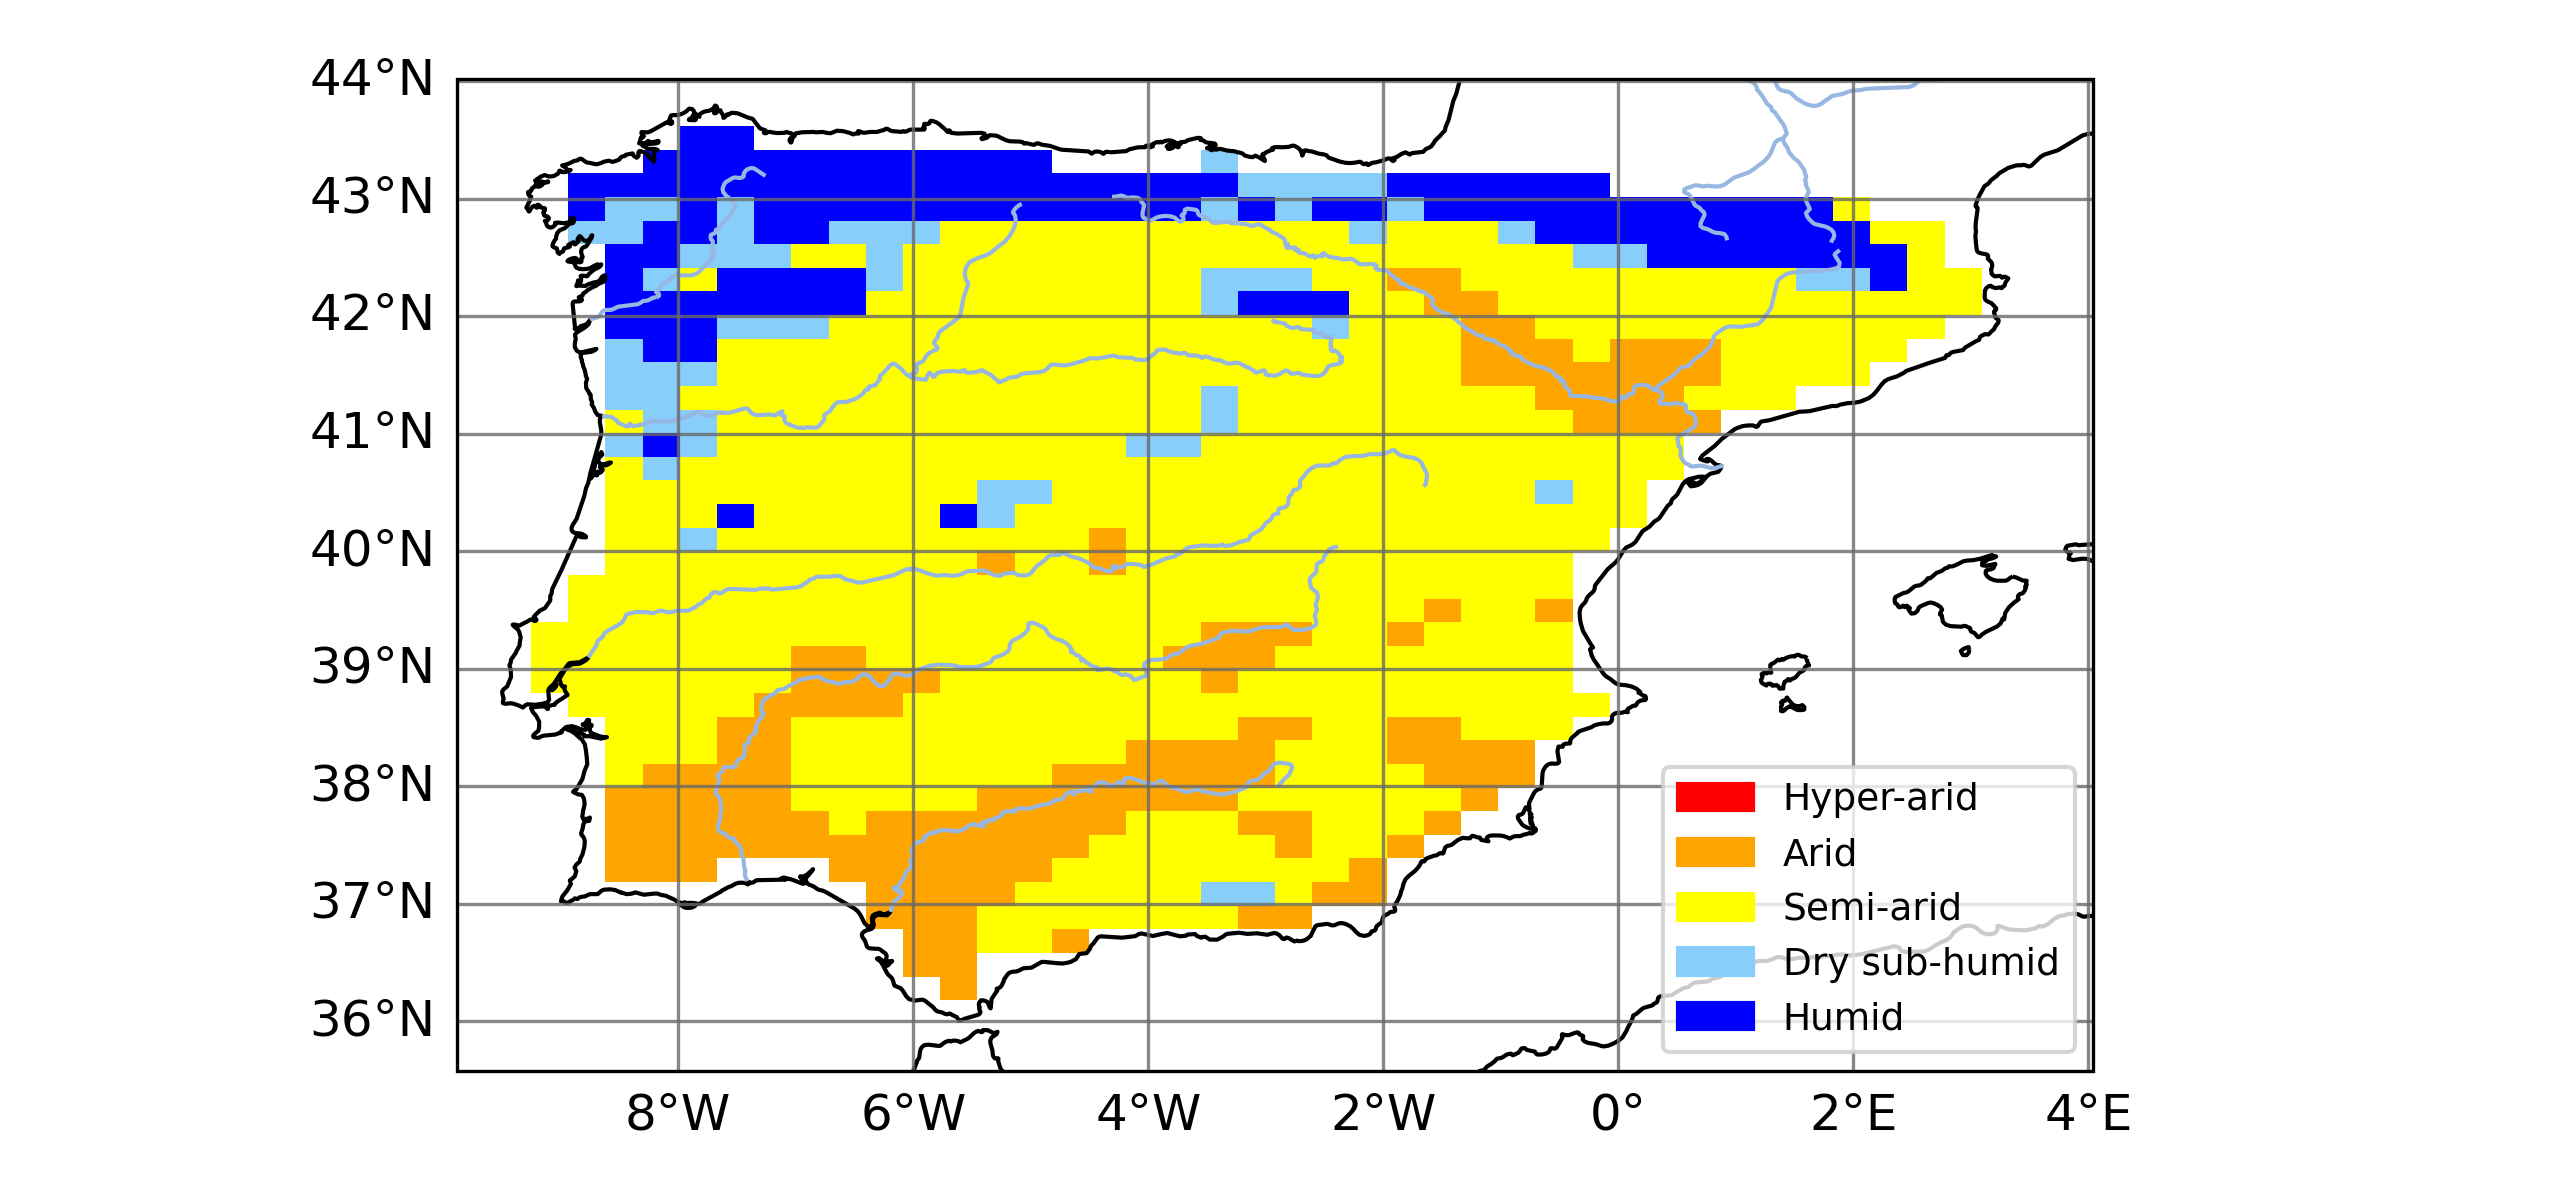
\includegraphics[width=\textwidth]{images/chap4/future/aridity_index_fut_irr.png}
    \end{subfigure}\\
    
    \vspace{1cm}

    \begin{subfigure}[b]{0.31\textwidth}
        \caption{Share of aridity index classes in \presnoirr}
        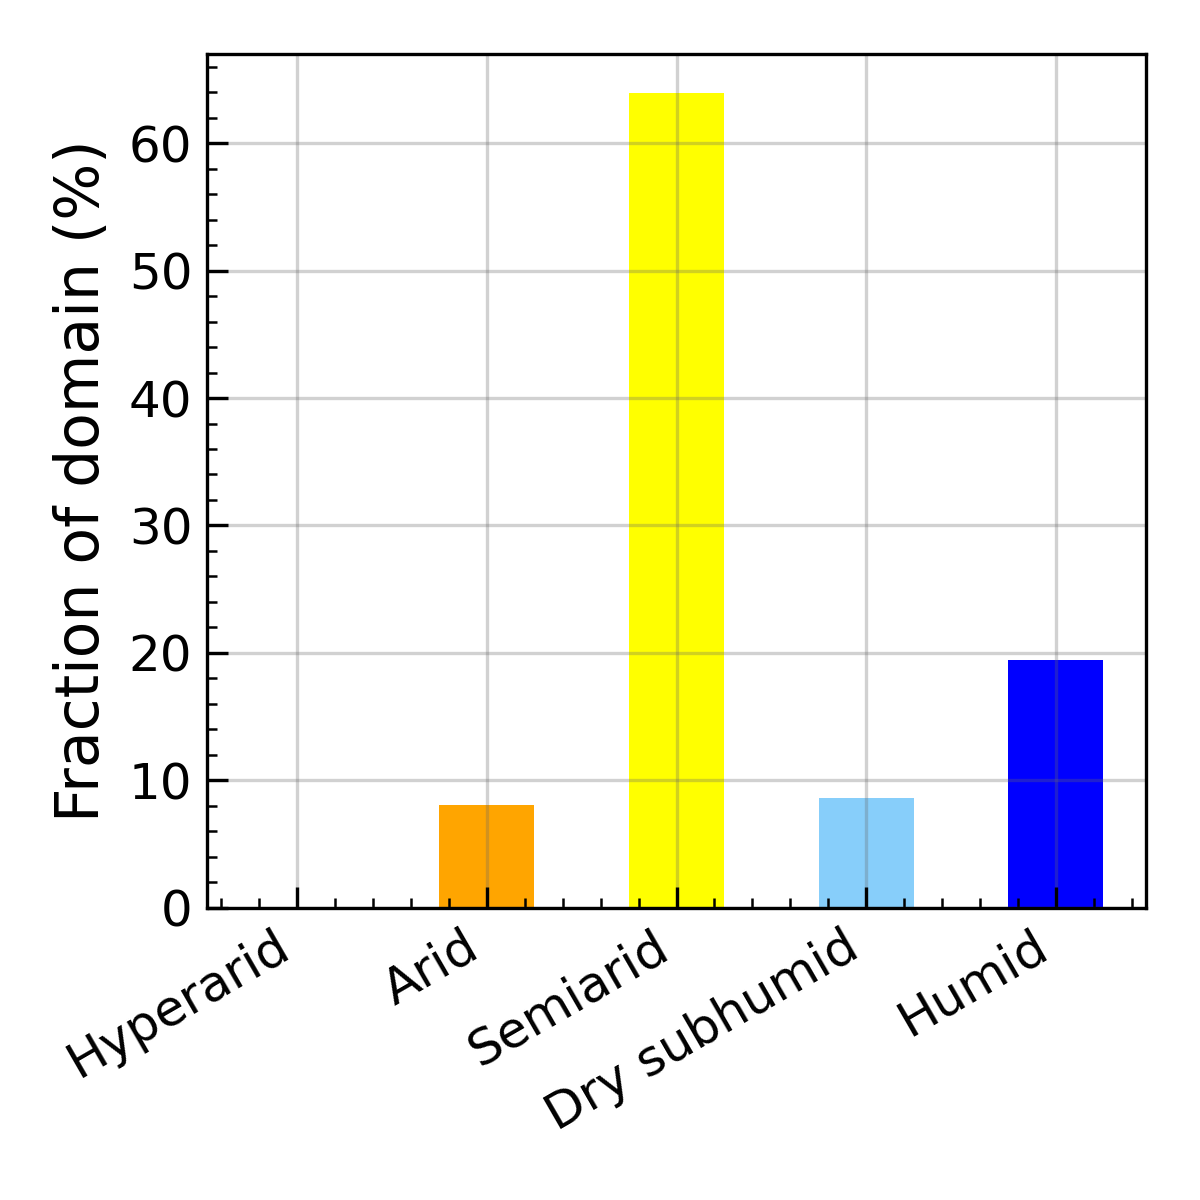
\includegraphics[width=\textwidth]{images/chap4/future/aridity_index_distribution_pres_noirr.png}
    \end{subfigure}
    \begin{subfigure}[b]{0.31\textwidth}
        \caption{Share of aridity index classes in \futnoirr}
        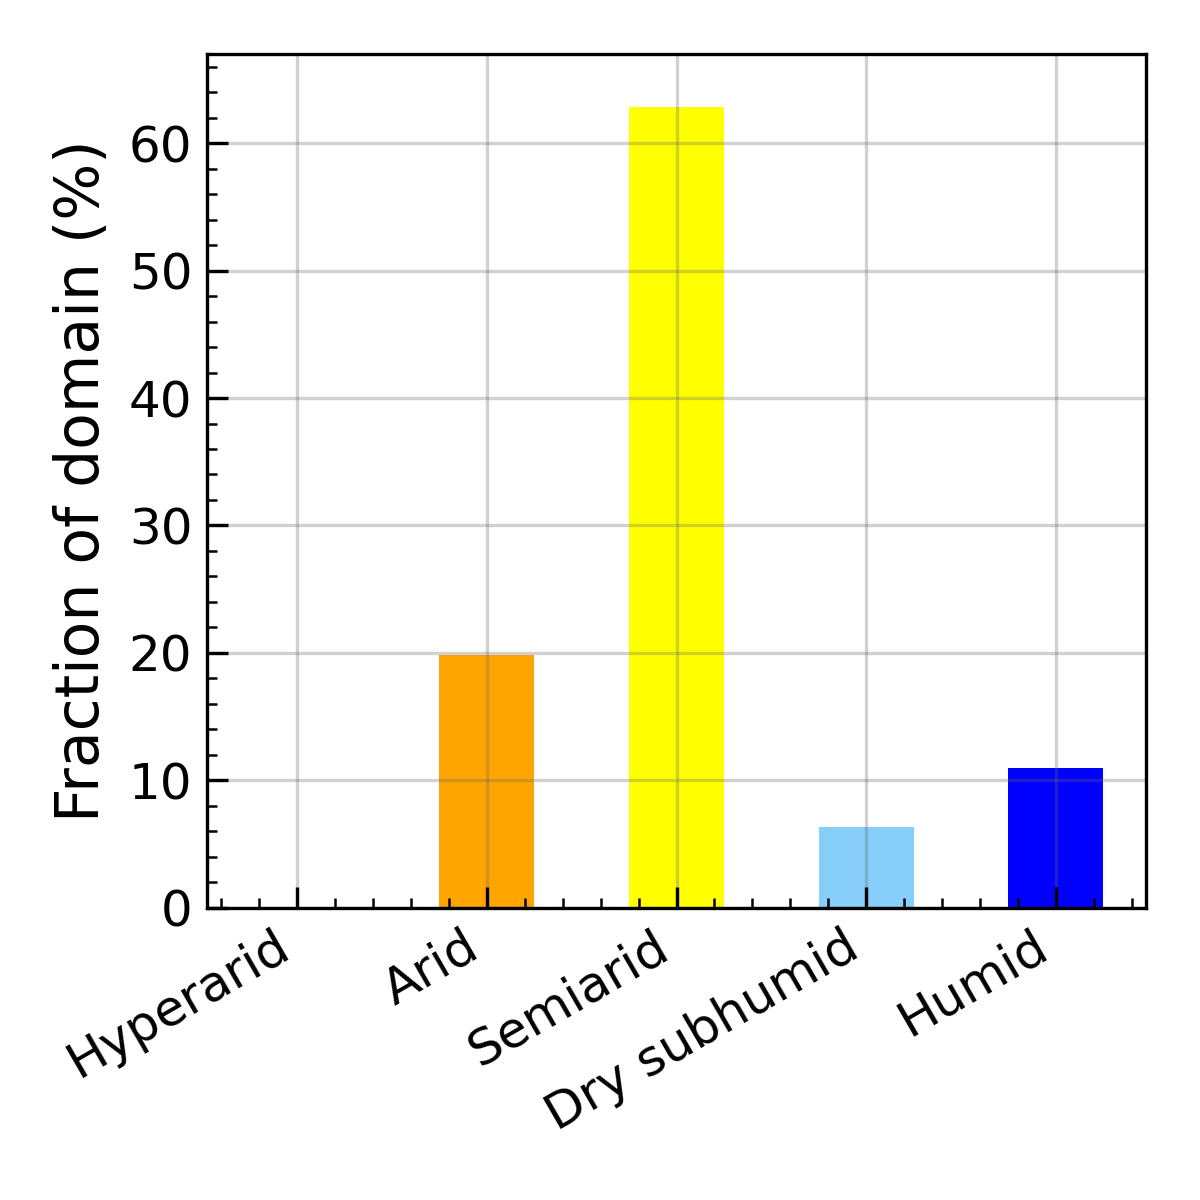
\includegraphics[width=\textwidth]{images/chap4/future/aridity_index_distribution_fut_noirr.png}
    \end{subfigure}
    \begin{subfigure}[b]{0.31\textwidth}
        \caption{Share of aridity index classes in \futirr}
        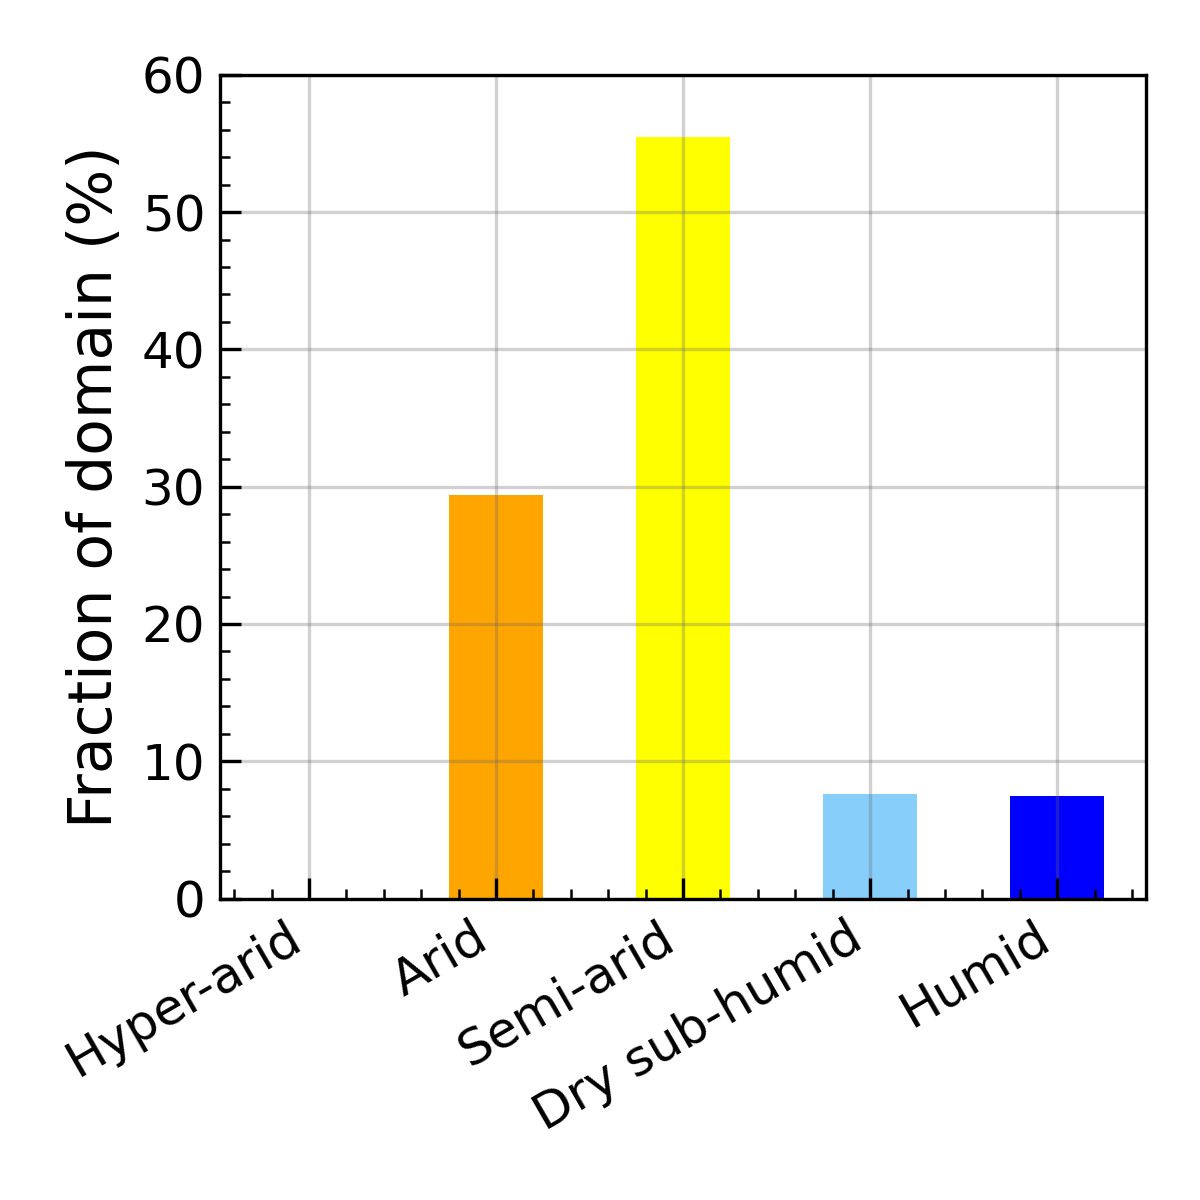
\includegraphics[width=\textwidth]{images/chap4/future/aridity_index_distribution_fut_irr.png}
    \end{subfigure}
    \caption{Spatial distribution of aridity index values and classes in the \presnoirr (2010-2022), \futnoirr (2050-2062), and \futirr simulations (2050-2062).}
    \label{fig:aridity_index_v2}
\end{figure}

% present_noirr
%Arid: 74 grid cells (8.034744842562432)
%Semiarid: 589 grid cells (63.952225841476654)
%Dry subhumid: 79 grid cells (8.577633007600435)
%Humid: 179 grid cells (19.435396308360477)

% future_noirr
%Arid: 183 grid cells (19.86970684039088)
%Semiarid: 579 grid cells (62.866449511400646)
%Dry subhumid: 58 grid cells (6.297502714440825)
%Humid: 101 grid cells (10.966340933767643)

% future_irr
%Arid: 150 grid cells (16.286644951140065)
%Semiarid: 601 grid cells (65.25515743756786)
%Dry subhumid: 59 grid cells (6.406080347448426)
%Humid: 111 grid cells (12.052117263843648)
